\section{Collisional-radiative modelling}
\label{sec:CR}

Fundamental to the calculation of the spectral radiation coefficients is the determination of the electronic level populations.
Under thermal equilibrium conditions, the level populations assume a Boltzmann distribution.
When insufficient collisions have occurred for thermal equilibrium to be achieved, the rate equation for each level must be considered.
The net population rate of level $i$ (also referred to in the literature as the `master-equation'~\cite{park_1990}) is the difference between the rate of transitions moving electrons in and out of the level:

\begin{equation}
 \frac{dN_\text{i}}{dt} = \left ( \frac{dN_\text{i}}{dt} \right )_\text{in} - \left ( \frac{dN_\text{i}}{dt} \right )_\text{out} \label{eq:CR_ME}
\end{equation}

Although multidimensional simulations with the collisional-radiative equations fully coupled with the flowfield have recently been performed (\textit{e.g.} Reference~\cite{panesi_phd}), this is computationally prohibitive for the time accurate Navier--Stokes calculations performed in the present work.
Rather, the quasi-steady-state (QSS) approximation proposed by Park~\cite{park_1990} is applied to decouple the solution from the temporal evolution of the flowfield.
The QSS approximation assumes the net population rate of level $i$ to be much smaller than the individual incoming and outgoing rates:

\begin{equation}
 \frac{dN_\text{i}}{dt} \ll \left ( \frac{dN_\text{i}}{dt} \right )_\text{in} \text{ , \hspace{1cm} and \hspace{1cm} }  \frac{dN_\text{i}}{dt} \ll \left ( \frac{dN_\text{i}}{dt} \right )_\text{out} \text{ . }\nonumber
\end{equation}

The net population rate-of-change in Equation~\ref{eq:CR_ME} can therefore be approximated as zero, and the QSS solution is found when the incoming and outgoing rates are balanced:

\begin{equation}
 0 = \left ( \frac{dN_\text{i}}{dt} \right )_\text{in} - \left ( \frac{dN_\text{i}}{dt} \right )_\text{out} \label{eq:QSS_condition}
\end{equation}

As the population rates are functions of the immediate flow state only, the QSS solution is decoupled from the temporal evolution of the flowfield.
However the QSS approximation is known not to be valid for the ground state~\cite{park_1990}.
The QSS approximation is therefore only applied to the excited levels, and the ground state population is solved by considering the number density balance for the species:

\begin{equation}
 N_{i=1} = N_\text{total} - \sum_{i=2}^{N_\text{levels}} N_i \label{eq:QSS_closure}
\end{equation}

\subsection{Collisional-radiative mechanisms}

The collisional-radiative mechanisms considered in the present work are:

\begin{enumerate}
 \item Heavy particle impact excitation,
 \item Electron impact excitation,
 \item Heavy particle impact dissociation,
 \item Electron impact dissociation,
 \item Electron impact ionisation, and
 \item Bound-bound radiative transitions.
\end{enumerate}

Free-bound radiative transitions are omitted as the depopulation rates due to bound-bound radiative transitions are considerably more significant for the conditions of interest~\cite{JohnPhd}.

% Huo (2008) notes that radiative-recombination may be very significant, but doesn't really justify this statement

\subsubsection{Heavy particle impact excitation}

Heavy particle impact excitation reactions have the following form:

\begin{equation}
 \text{X}_i + \text{M} \leftrightharpoons  \text{X}_j + \text{M}
\end{equation}

\noindent where M denotes an arbitrary heavy particle species, X denotes an arbitrary atomic species and $i$ and $j$ denote the lower (initial) and upper (final) electronic levels respectively.
The net population rate of level $i$ due to heavy particle impact excitation (HPIE) reactions is:

\begin{equation}
 \left ( \frac{dN_\text{i}}{dt} \right )_\text{HPIE} =  \sum_{j \neq i} K_{M}(j,i) N_{j} N_{M} - \sum_{j \neq i} K_{M} (i,j) N_{i} N_{M} 
\end{equation}

\par

In the present work, heavy particle impact excitation processes are only considered for diatomic species as the electron impact mechanisms dominate in the flow regime where atomic nonequilibrium is significant~\cite{park_1990,JohnPhd}.
The forward rate coefficients for heavy particle impact excitation are obtained from the literature in generalised Arrhenius form:

\begin{equation}
 K_{M}(i,j) = C T_x^n \text{exp} \left ( - \frac{E_a}{k T_x} \right ) \label{eq:CR_GA}
\end{equation}

\noindent where the rate controlling temperature for the excitation process is the geometric average of the translational and vibrational temperatures:

\begin{equation}
 T_x = \sqrt{T_\text{trans} T_\text{vib.}}
\end{equation}

The backward reaction rate coefficients are calculated via the principal of detailed balancing:

\begin{equation}
 K_{M}(j,i) = \left [ K_{M}(i,j) \frac{Q_i}{Q_j} \right ]_{T_\text{trans}} \label{eq:K_b_HPIE}
\end{equation}

\noindent where $Q_i$ and $Q_j$ are the partition functions of the lower and upper electronic levels respectively.
The rate controlling temperature for the de-excitation process is the translational temperature, and therefore $K_{M}(i,j)$, $Q_i$ and $Q_j$ in Equation~\ref{eq:K_b_HPIE} are evaluated at $T_\text{trans}$. 

% Johnston~\cite{JohnPhd} compiled rates for the most important heavy particle impact excitation processes for N$_2^+$ and N$_2$ from the literature for application to lunar return air shock layers.
% Park~\cite{park2008b} presents a comprehensive set of heavy particle impact excitation rates for N$_2$, N$_2^+$, O$_2$, NO, CO and CN.
% The rates are derived from collision cross sections which are based on laser and shock tube induced quenching experiments and estimated where no experimental data is available.
% Zalogin~\cite{zalogin_2001} included heavy particle impact excitation reactions for C$_2$, CO and CN in a collisional-radiative model for shock heated CO$_2$--N$_2$ mixtures.

\subsubsection{Electron impact excitation}

Electron impact excitation reactions have the following form:

\begin{equation}
 \text{X}_i + \text{e}^- \leftrightharpoons  \text{X}_j + \text{e}^- + \text{e}^-
\end{equation}

The net population rate of level $i$ due to electron impact excitation (EIE) reactions is:

\begin{equation}
 \left ( \frac{dN_\text{i}}{dt} \right )_\text{EIE} =  \sum_{j \neq i} K_{e}(j,i) N_{j} N_{e} - \sum_{j \neq i} K_{e} (i,j) N_{i} N_{e} 
\end{equation}

The forward rate coefficients are assumed to be governed by the free electron temperature $T_e$, and the backward reaction rate coefficient is calculated via the principal of detailed balancing:

\begin{equation}
 K_{e}(j,i) = \left [ K_{e}(i,j) \frac{Q_i}{Q_j} \right ]_{T_e}
\end{equation}

\noindent where the de-excitation process is assumed to be governed by the free electron temperature $T_e$.

\par

Electron impact excitation processes for both diatomic and atomic species are considered in the present work.
The forward rate coefficients for diatomic electron impact excitation are either obtained directly from the literature in generalised Arrhenius form, or calculated by integrating cross sections.
In the present work, the following method proposed by Park~\cite{park_1990} for calculating the diatomic electron impact excitation rate coefficient from the respective cross section is implemented:

\begin{equation}
 K_e (i,j) = \frac{S \sum_{v_i} \sum_{v_j} q(v_i, v_j) \text{exp} \left [ - \frac{G_{v_i}}{k T_\text{vib.}} \right ] }{\frac{kT_r}{B_{e,i}} Q_{\text{vib.},i} } \label{eq:within}
\end{equation}

\noindent where $q(v_i, v_j)$ is the Frank-Condon factor for the vibronic transition between $v_i$ and $v_j$, $G_{v_i}$ is the vibrational energy of vibrational state $v_i$ and $Q_{\text{vib.},i}$ is the vibrational partition function for electronic level $i$.
The parameter $S$ is defined as:

\begin{equation}
 S = 5.47 \times 10^{-11} \sqrt{T_e} \text{exp} \left ( - \frac{\mathrm{T}_j + G_{v,j} - \mathrm{T}_i - G_{v,i} }{k_B T_e} \right )
\end{equation}

\noindent where $I$	 is:

\begin{equation}
 I = \left ( \frac{B_{e,j} - B_{e,i}}{k_B T_e} + \frac{B_{e,i}}{k_B T_\text{rot.}} \right )^{-3/2} \left [ C \Gamma(1.5) B D \Gamma(2.5) \right ]
\end{equation}

with:

\begin{eqnarray}
 C &=& \frac{\mathrm{T}_j + G_{v,j} - \mathrm{T}_i - G_{v,i} }{k_B T_e} B + A \text{ , } \\
 D &=& \frac{B_{e,j} - B_{e,i}}{k_B T_e} \left ( \frac{B_{e,j} - B_{e,i}}{k_B T_e} + \frac{B_{e,i}}{k_B T_e} \right )^{-1} \text{ . }
\end{eqnarray}

\noindent The parameters $A$ and $B$ are defined as:

\begin{eqnarray}
 A &=& \int_0^\infty \left [ \frac{\sigma(\xi)}{\pi a_0^2} \right ] \text{exp} ( -\xi ) \xi d \xi \\
 B &=& \int_0^\infty \left [ \frac{\sigma(\xi)}{\pi a_0^2} \right ] \text{exp} ( -\xi ) d \xi  \label{eq:without}
\end{eqnarray}

\noindent where $a_0$ is the first Bohr radius and $\sigma$ is the electron impact excitation cross section with $\xi = x -1$ and $x = E / E^\ast$ where $E$ is the electron energy and $E^\ast$ is the threshold energy ($\Delta \mathrm{T}_e$).

\par

Although experimental and theoretical electron impact excitation cross sections for atomic species are available for some transitions from low lying states, for the majority of transitions we must rely on semi-empirical models.
Here we will briefly describe the approximate electron impact excitation models considered for atoms, whilst a detailed description of the rate coefficient models selected for each species will be presented later.

\par

Numerous empirical electron impact excitation models for atomic species were investigated in the comprehensive studies of Johnston~\cite{JohnPhd} and Panesi~\cite{panesi_phd}.
As a baseline model, Panesi~\cite{panesi_phd} implemented electron impact excitation reaction rate coefficients obtained by analytical integration of the Drawin~\cite{drawin_1968} cross sections over a Maxwell-Boltzmann velocity distribution:

\begin{eqnarray}
 K_e (i,j) &=& \left \lbrace \begin{array}{cc} \sqrt{ \frac{8 k_B T_e}{\pi m_e} } 4 \pi a_0^2 \alpha \left ( \frac{I_H}{k T_e} \right )^2 I_1 (a ) & \text{ for an optically allowed transition } \\ \sqrt{ \frac{8 k_B T_e}{\pi m_e} } 4 \pi a_0^2 \alpha \left ( \frac{E_j - E_i}{k_B T_e} \right )^2 I_2 (a ) & \text{ for an optically forbidden transition } \end{array} \right . \nonumber \\
 \label{eq:drawin_rates}
\end{eqnarray}
 
\noindent where $m_{e}$ is the mass of an electron, $a_{0}$ is the first Bohr radius, $\alpha = 0.05$, $I_H$ is the ionisation energy of the hydrogen atom from the ground state and $I_{1}(a)$ and $I_{2}(a)$ are calculated as:

\begin{eqnarray}
 I_1(a) &=& 0.63255 a^{-1.6454} e^{-a}, \text{ \hspace{1cm} where \hspace{1cm} } a = \frac{E_{j}-E_{i}}{k_B T} \\
 I_2(a) &=& 0.23933 a^{-1.4933} e^{-a}, \text{ \hspace{1cm} where \hspace{1cm} } a = \frac{E_{\text{ionise},i}-E_{i}}{k_B T}
\end{eqnarray}

The hydrogenic model of Gryzinksi~\cite{Gryz59} was implemented by both Johnston~\cite{JohnPhd} and Panesi~\cite{panesi_phd}.
Similarly as for the Drawin model, the Gryzinksi model is semi-empirical and universally applicable to all transition types.
The electron impact excitation reaction rate coefficients are calculated by integrating the Gryzinksi cross section $\sigma_{ij}$ over a Maxwellian velocity distribution:

\begin{eqnarray}
 K_{e} (i,j) = \frac{8\pi}{\sqrt{m}} \left ( \frac{1}{2\pi m k_B T_e} \right )^{1.5} && \left [ \int_{\Delta E_{i,j}}^{\infty} \sigma_{i,j} (E) \text{exp}\left ( - \frac{E}{k_B T_{e}} \right ) E dE \right . \nonumber \\
  &+& \left . \int_{\Delta E_{i,j+1}}^{\infty} \sigma_{i,j+1} (E) \text{exp}\left ( - \frac{E}{k_B T_{e}} \right ) E dE \right] 
\end{eqnarray}

\noindent where $\sigma_{ij}(E)$ is given by Eq.~\ref{eq:sigma_ij_1} for $\Delta E_{ij} + E_{\text{ionise}} - E_{i} \leq E$ and by Eq.~\ref{eq:sigma_ij_2} for $\Delta E_{ij} + E_{\text{ionise}} - E_{i} \geq E$:

\begin{eqnarray}
 \sigma_{i,j}(E) &=& \frac{4.2484 \times 10^{-6}}{\Delta E_{ij}^2}\left ( \frac{E}{E_{\text{ionise}} - E_{i} + E} \right )^{1.5} \nonumber \\ 
 &\times& \left \lbrace \frac{2}{3} \left [ \frac{E_{\text{ionise}} - E_{i}}{E} + \frac{\Delta E_{i,j}}{E} \left ( 1 - \frac{E_{\text{ionise}} - E_{i}}{E} \right ) - \left ( \frac{\Delta E_{i,j}}{E} \right )^{2} \right ] \right \rbrace  \nonumber \\ \label{eq:sigma_ij_1}
\end{eqnarray}

\begin{eqnarray}
 \sigma_{i,j}(E) &=& \frac{4.2484 \times 10^{-6}}{\Delta E_{ij}^2}\left ( \frac{E}{E_{\text{ionise}} - E_{i} + E} \right )^{1.5} \nonumber \\ 
 &\times& \left \lbrace \frac{2}{3} \left [ \frac{E_{\text{ionise}} - E_{i}}{E} + \frac{\Delta E_{i,j}}{E} \left ( 1 - \frac{E_{\text{ionise}} - E_{i}}{E} \right ) - \left ( \frac{\Delta E_{i,j}}{E} \right )^{2} \right ] \right . \nonumber \\
 &\times& \left . \left [ \left ( 1 + \frac{\Delta E_{ij} }{E_{\text{ionise}} - E_i} \right ) \left( 1 - \frac{\Delta E_{i,j}}{E} \right ) \right ]^{0.5} \right \rbrace \nonumber \\ \label{eq:sigma_ij_2}
\end{eqnarray}

\noindent In the present implementation the cross section integration is performed by a change of variables to shift the limits to [-1,1] and applying 10 point Gaussian quadrature.

\par

Johnston~\cite{JohnPhd} and Panesi~\cite{panesi_phd} also considered the empirical models proposed by Allen~\cite{Allen62}, Van Regmorter~\cite{VG62} and Park~\cite{Park73,park_1990}.
Both authors found the Park~\cite{Park73,park_1990} models to give substantially larger rates than other more accurate models for electron impact excitation of N and O, and were therefore not implemented.
Although Johnston~\cite{JohnPhd} preferenced the models of Allen~\cite{Allen62} and Van Regmorter~\cite{VG62} over that of Gryzinski~\cite{Gryz59}, Panesi~\cite{panesi_phd} found the Drawin model described in Equation~\ref{eq:drawin_rates}  to be in good agreement with these models.
Therefore in the present work only the Gryzinski~\cite{Gryz59} and Drawin~\cite{drawin_1968} empirical models will be considered.

\subsubsection{Heavy particle impact dissociation}

Heavy particle impact dissociation reactions have the following form:

\begin{equation}
 \text{AB}_i + \text{M} \leftrightharpoons  \text{A} + \text{B} + \text{M}
\end{equation}

\noindent where A and B are the constituent atoms of the diatomic molecule AB.
The net population rate of level $i$ due to heavy particle impact dissociation (HPID) reactions is:

\begin{equation}
 \left ( \frac{dN_\text{i}}{dt} \right )_\text{HPID} =  K_{M}(d,i) N_\text{A} N_\text{B} N_{M} - K_{M} (i,d) N_{i} N_{M} 
\end{equation}

\noindent where $d$ denotes the dissociated state.
The forward rate coefficients for diatomic heavy particle impact dissociation are obtained from the literature in generalised Arrhenius form, where the rate controlling temperature for the excitation process is the geometric average of the translational and vibrational temperatures:

\begin{equation}
 T_x = \sqrt{T_\text{trans} T_\text{vib.}}
\end{equation}

The heavy particle impact recombination rate coefficient is related to the heavy particle impact dissociation rate coefficient via the principal of detailed balancing:

\begin{equation}
 K_{M}(d,i) = \left [ K_{M}(i,d) \frac{Q_i}{Q_\text{A} Q_\text{B}} \right ]_{T_\text{trans}}
\end{equation}

\noindent where the total partition functions $Q$ must include the formation energy contribution $\text{exp} \left ( - h_f / k_B T_\text{trans} \right )$ to account for the dissociation potential of the lower state, and the rate controlling temperature for the de-excitation process is the translational temperature $T_\text{trans}$. 

\subsubsection{Electron impact dissociation}

Similarly as for heavy particle impact dissociation, electron impact dissociation reactions have the following form:

\begin{equation}
 \text{AB}_i + \text{e}^- \leftrightharpoons  \text{A} + \text{B} + \text{e}^-
\end{equation}

\noindent where A and B are the constituent atoms of the molecule AB.
The net population rate of level $i$ due to electron impact dissociation (EID) reactions is:

\begin{equation}
 \left ( \frac{dN_\text{i}}{dt} \right )_\text{EID} =  K_{e}(d,i) N_\text{A} N_\text{B} N_{e} - K_{e} (i,d) N_{i} N_{e} 
\end{equation}

\noindent where $c$ denotes the ionised state.
The forward rate coefficients for diatomic electron impact dissociation are obtained from the literature in generalised Arrhenius form, where the rate controlling temperature for the dissociation process is the free electron temperature:

\begin{equation}
 T_x = T_e
\end{equation}

The electron impact recombination rate coefficient is calculated via the principal of detailed balancing:

\begin{equation}
 K_{e}(d,i) = \left [ K_{e}(i,d) \frac{Q_i}{Q_\text{A} Q_\text{B}} \right ]_{T_e}
\end{equation}

\noindent where the total partition functions $Q$ must include the formation energy contribution $\text{exp} \left ( - h_f / k_B T_\text{trans} \right )$ to account for the dissociation potential of the lower state, and the rate controlling temperature for the recombination process is assumed to be the free electron temperature $T_e$.

\subsubsection{Electron impact ionisation}

Electron impact ionisation reactions have the following form:

\begin{equation}
 \text{X}_i + \text{e}^- \leftrightharpoons  \text{X}^+ + \text{e}^- + \text{e}^-
\end{equation}

\noindent where $\text{X}^+$ is the ionised species.
The net population rate of level $i$ due to electron impact excitation (EII) reactions is:

\begin{equation}
 \left ( \frac{dN_\text{i}}{dt} \right )_\text{EII} =  K_{e}(c,i) N_\text{ion} N_{e} N_{e} - K_{e} (i,c) N_{i} N_{e} 
\end{equation}

\noindent where $c$ denotes the ionised states.
The ionisation process is assumed to be governed by the free electron temperature $T_e$, and the electron impact recombination rate coefficient is related to the electron impact ionisation rate coefficient via the principal of detailed balancing:

\begin{equation}
 K_{e}(c,i) = \left [ K_{e}(i,c) \frac{Q_i}{Q_\text{ion} Q_e} \right ]_{T_e}
\end{equation}

\noindent where the total partition functions $Q$ must include the formation energy contribution $\text{exp} \left ( - h_f / k_B T_\text{trans} \right )$ to account for the ionisation potential of the lower state, and the rate controlling temperature for the recombination process is assumed to be the free electron temperature $T_e$.

\par

Electron impact ionisation processes are only considered for atomic species in the present work, as the dissociation and excitation processes are much more significant for diatomic species.
Similarly as for electron impact excitation, electron impact ionisation rate coefficients based on experimental measurements or theoretical calculations are preferred in the present work.
The ionisation cross sections, however, are typically only provided for low lying states and we must rely on empirical models for the remainder.
Two empirical models for electron impact ionisation are considered, both based on the hydrogenic cross sections of Drawin~\cite{drawin_1968}.
The model implemented by Johnston~\cite{JohnPhd} gives the electron impact ionisation reaction rate coefficients as:

\begin{equation}
 K_{e}(i,c) = 1.46 \times 10^{-10} \sqrt{ T_e } \left ( \frac{I_H}{I - E_i} \right )^2 \zeta y \psi_1 ( y )
\end{equation}

\noindent where the number of equivalent electrons $\zeta$ is 3 for ground electronic states and 1 for excited states and $y$ is the reduced energy of the incoming electrons:

\begin{equation}
 y = \frac{I - E_i}{k_B T_e} \text{ , }
\end{equation}

\noindent and the function $\psi_1$ is:

\begin{equation}
 \psi_1 ( y ) = \frac{\text{exp}( -y)}{1 + y} \left \lbrace \frac{1}{20 + y} + \text{ln} \left [ 1.25 \left ( 1 + \frac{1}{y} \right ) \right ] \right \rbrace
\end{equation}

Panesi~\cite{panesi_2008a,panesi_phd} implemented another model for electron impact ionisation that is also based on the Drawin cross sections.
For this model the ionisation rate coefficients are calculated by the optically allowed expression presented in Equation~\ref{eq:drawin_rates} with $\alpha=1$ and $a = ( I - E_i ) / ( k_B T_e )$.

\subsubsection{Bound-bound radiative transitions}

Bound-bound radiative transitions have the following form:

\begin{equation}
 \text{X}_j \leftrightharpoons \text{X}_i + h \nu
\end{equation}

\noindent where the emitted photon energy is equivalent to the energy difference between the two levels:

\begin{equation}
 h \nu = E_j - E_i
\end{equation}

The net population rate of level $i$ due to bound-bound radiative transitions (BBRT) is:

\begin{equation}
 \left ( \frac{dN_\text{i}}{dt} \right )_\text{BBRT} =  \sum_{j > i} \Lambda_{j,i} A(j,i) N_j - \sum_{j < i} \Lambda_{i,j} A(i,j) N_i 
\end{equation}

\noindent where $A(i,j)$ is the spontaneous transition probability from level $i$ to level $j$ and $\Lambda_{i,j}$ is the associated escape factor.
For atomic radiators, the total transition probability between two nonequilibrium electronic levels is calculated by averaging the degeneracy weighted transition probabilities for all transitions between the two levels:

\begin{equation}
 A(i,j) = \frac{\sum_{i^\prime} \sum_{j^\prime} g_i^\prime A(i^\prime,j^\prime)}{\sum_{i^\prime} \sum_{j^\prime} g_i^\prime} \label{eq:A_av}
\end{equation}

\noindent where $i^\prime$ and $j^\prime$ denote sub-levels belonging to grouped-levels $i$ and $j$ respectively.
For diatomic radiators, the total transition probability between two nonequilibrium electronic levels can be calculated either from radiative lifetimes $\gamma_{i,j}$ where available:

\begin{equation}
 A(i,j) = \frac{1}{\gamma_{i,j}} \text{ , }
\end{equation}

\noindent or by averaging over the weighted vibrational transition probabilities~\cite{hyun_phd}:

\begin{equation}
 A(i,j) = \frac{\sum_{v_i} Q_{\text{vib.},v_i} \sum_{v_j} A_\text{vib.}(v_i,v_j)}{\sum_{v_i} Q_{\text{vib.},v_i}}  \label{eq:A_av_diatomic}
\end{equation}

\noindent where $ Q_{\text{vib.},v_i}$ is the vibrational partition function for vibrational level $v_i$ and {$A_\text{vib.}(v_i,v_j)$ is the vibrational transition probability corresponding to the $v_i,v_j$ band.
The inverse process of radiative absorption is accounted for by the escape factor $\Lambda$ that is the ratio of re-absorbed to emitted radiative energy\footnote{An escape factor of one represents an optically thin transition where no re-absorption occurs, while an escape factor of zero represents an optically thick transition where complete re-absorption occurs.}:

\begin{equation}
 \Lambda = \frac{E_\text{abs.}}{E_\text{em.}}
\end{equation}

As radiative re-absorption is determined by solving the radiation transport equations, the introduction of an escape factor here implies that the collisional-radiative and radiative transport equations should be solved in a coupled manner.
Unfortunately such a procedure is computationally prohibitive, and therefore the escape factor is approximated in the present work --- specifically, solutions with optically thick and optically thin transitions are presented, providing approximate lower and upper bounds for the solution space.

% \subsubsection{Free-bound radiative transitions}

% Free-bound radiative transitions result from an ion and an electron recombining and have the following form:

% \begin{equation}
% \text{X}^+ + \text{e}^- \leftrightharpoons  \text{X}_i + h \nu
% \end{equation}

% \noindent where the reverse process is photoionisation (\textit{i.e.} absorption of radiative energy providing the energy for the atom or molecule to be ionised).
% The net population rate of level $i$ due to free-bound radiative transitions (FBRT) is:

% \begin{equation}
%  \left ( \frac{dN_\text{i}}{dt} \right )_\text{FBRT} =  \Lambda_{c,i} A(c,i) N_\text{ion} N_e
% \end{equation}

% \noindent where reabsorption is accounted for by the escape factor $\Lambda$ in a similar fashion as for bound-bound transitions.
% For consistency with the spectral radiation model, free-bound transitions in the present work are only considered for atomic species.

\subsection{Master equation formulation and solution}

The implemented master equation for an electronic level $i$ is:

\begin{eqnarray}
  \frac{\partial N_{i}}{\partial t} =&& \overbrace{\sum_{j \neq i} K_{e}(j,i)N_{j}N_{e} - \sum_{j \neq i} K_{e} (i,j)N_{i}N_{e} }^{\text{electron impact excitation}} \nonumber \\
 &+& \overbrace{\sum_{j \neq i} K_{M}(j,i)N_{j}N_{M} - \sum_{j \neq i} K_{M} (i,j)N_{i}N_{M} }^{\text{heavy particle impact excitation}} \nonumber \\
 &+& \overbrace{ K_{e}(c,i)N_{+}N_{e}^{2} - K_{e}(i,c)N_{i}N_{e} }^{\text{electron impact ionisation}} + \overbrace{ K_{e}(d,i)N_{XY}N_{e} - K_{e}(i,d)N_{i}N_{e} }^{\text{electron impact dissociation}} \nonumber \\
 &+& \overbrace{ \sum_{j > i} \Lambda_{j,i} A(j,i)N_{j} - \sum_{j < i} \Lambda_{i,j}A(i,j)N_{i} }^{\text{radiative excitation}}, \label{eq:dNidt}
\end{eqnarray}

As quenching or exchange reactions amongst different species are not considered in the present work, a linear QSS system can be formulated independently for each nonequilibrium radiator.
For a radiator with $N_\text{levels}^\ast$ nonequilibrium electronic levels\footnote{As will be discussed, the number of nonequilibrium electronic levels $N_\text{levels}^\ast$ is not necessarily the total number of electronic levels $N_\text{levels}$}, the QSS system is formed by considering the master equations (see Equation~\ref{eq:dNidt}) for non-ground states in the QSS limit (see Equation~\ref{eq:QSS_condition}) with closure provided by the total population of the radiator (see Equation~\ref{eq:QSS_closure}).
The resulting system can be expressed in matrix form as:

\begin{equation}
 \boldsymbol{M} \vec{x} = \vec{b} \label{eq:Mx_b}
\end{equation}

\noindent where $\boldsymbol{M}$ is a square matrix of dimension $N_\text{levels}^\ast$ and $\vec{x}$ and $\vec{b}$ are vectors of dimension $N_\text{levels}^\ast$.
The elements of $\boldsymbol{M}$ are:

\begin{eqnarray}
 \boldsymbol{M}(i=1,j) &=& 1 + \sum_{j^\ast}^{N_{\text{eqs}}} f_{\text{eq.},j^\ast} \nonumber \\
 \boldsymbol{M}(i\neq1,j = i) &=& - \left [ \sum_{k \neq i} \left ( K_{M}(i,k)N_{M} + K_{e}(i,k)N_{e} \right ) + K_{e}(i,c)N_{e} \right . \nonumber \\
                               & & \left . + K_{M}(i,d)N_{M} + K_{e}(i,d)N_{e} + \sum_{k < i } \left ( \Lambda_{i,k}A(i,k) \right ) \right ] \nonumber \\
\boldsymbol{M}(i\neq1,j \neq i) &=& \left \lbrace \begin{array}{cc} K_{e}(j,i)N_{e} + K_{M}(j,i)N_{M} & \text{   for   } j < i \\ \\ K_{e}(j,i)N_{e} + K_{M}(j,i)N_{M} + \Lambda_{j,i}A(j,i) & \text{   for   } j > i \end{array} \right . \nonumber \\ \label{eq:M_elements} 
\end{eqnarray}

\noindent and the elements of $\vec{b}$ are:

\begin{eqnarray}
 \vec{b}(i=1) &=& N_{s} \nonumber \\
 \vec{b}(i\neq1) &=& - K_{e}(i,c)N_{e} - K_{M}(i,d)N_{M} - K_{e}(i,d)N_{e} - \Lambda_{c,i} A(c,i) N_{+} N_{e} \label{eq:b_elements}
\end{eqnarray}

\noindent where $N_s$ is the total species number density from the CFD solver.
The elements of $\vec{x}$ are the nonequilibrium level number densities:

\begin{equation}
 \vec{x}(i) = N_i
\end{equation}

The matrix line corresponding to the ground state ($i=1$) is the population summation from Equation~\ref{eq:QSS_closure}, while the remaining matrix lines are each of the master equations from Equation~\ref{eq:dNidt}
As mentioned previously, the nonequilibrium levels may be a sub-set of the electronic levels for the species.
A level not considered by the collisional-radiative model with index $j^\ast$ can be equilibrated with a nonequilibrium level $j$ by the Boltzmann equation:

\begin{equation}
 N_{j^\ast} = N_j \frac{Q_{\text{int},{j^\ast}}}{Q_{\text{int},{j}}} = N_j  f_{\text{eq.},j^\ast} \label{eq:F_eq}
\end{equation}

\noindent where $Q_{\text{int,}{j^\ast}}$ and $Q_{\text{int,}{j^\ast}}$ are the internal partition functions of the equilibriated and nonequilibrium levels respectively, and the ratio of these two partition functions is defined as the Boltzmann equilibrium factor $f_{\text{eq.},j^\ast}$.
To correctly account for the level equilibration in the collisional-radiative model, the $\boldsymbol{M}(i=1,j)$ matrix elements must include the sum of all Boltzmann equilibrium factors for nonequilibrium level $j$:

\begin{equation}
 \sum_{j^\ast}^{N_{\text{eqs}}} f_{\text{eq.},j^\ast}
\end{equation}

\par

Equation~\ref{eq:Mx_b} can then be easily solved via direct matrix inversion:

\begin{equation}
 \vec{x} = \boldsymbol{M}^{-1} \vec{b} \label{eq:x_Minvb}
\end{equation}

\noindent where $\boldsymbol{M}^{-1}$ is calculated via Gaussian elimination in the current implementation of the model.
At low temperatures, however, there are insufficient collisions for the QSS condition (Equation~\ref{eq:QSS_condition}) to remain valid, and the results of Equation~\ref{eq:x_Minvb} cannot be used.
Therefore in the present work the electronic levels of nonequilibrium radiators are assumed to be in Boltzmann distributions for free electron temperatures of 2,000\,K and under. 

\subsection{Collisional-radiative model for N$_2$--O$_2$ mixtures}

\begin{figure}[p]
 \centering
 \subfloat[Number density profile]{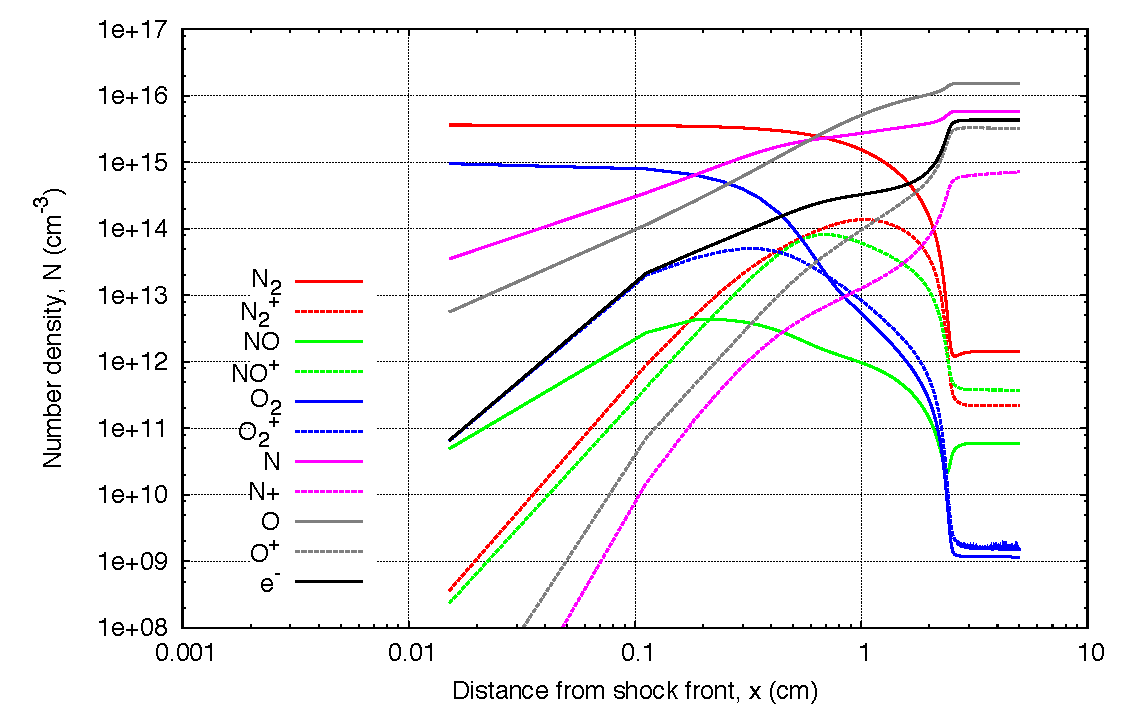
\includegraphics[width=0.9\linewidth]{collisional-radiative-modelling/figures/FireII_1634s_number_densities.pdf} \label{fig:FireII_1634s_number_densities}} \\
 \subfloat[Radiative emission profile]{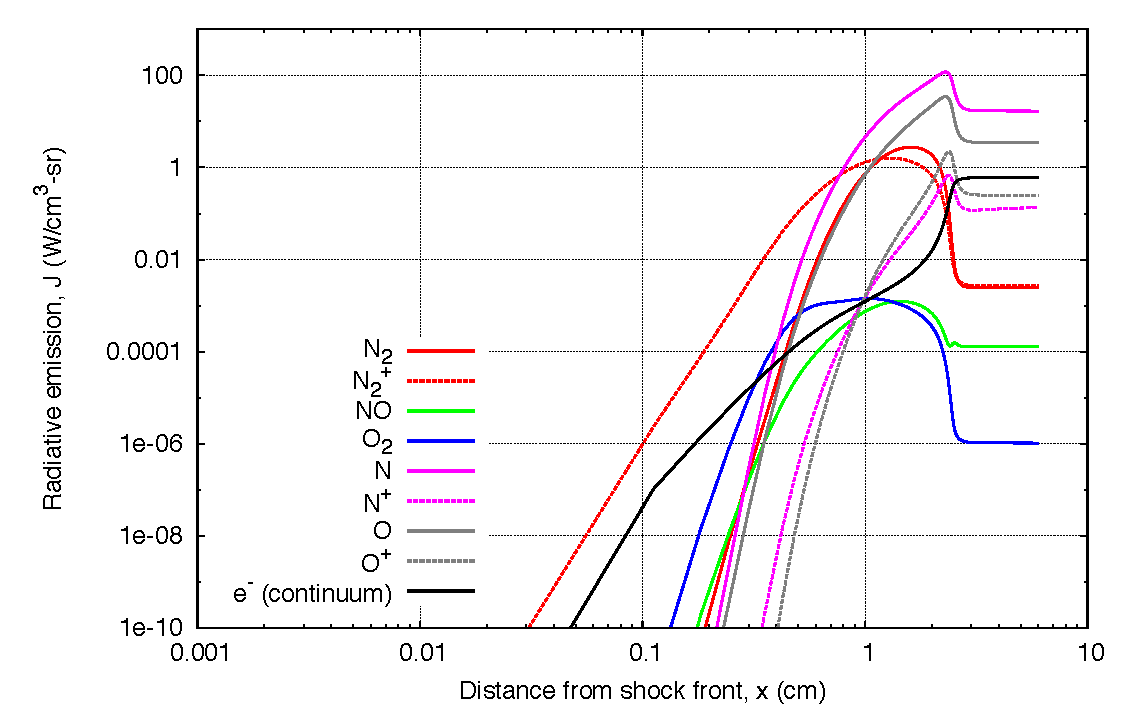
\includegraphics[width=0.9\linewidth]{collisional-radiative-modelling/figures/FireII_1634s_emissions.pdf} \label{fig:FireII_1634s_emissions}}
 \caption{Post-shock species number density and radiative emission profiles along the stagnation streamline of the Fire II $t=1634$\,s condition ($p_\infty = 2$\,Pa, $T_\infty = 195$\,K, $u_\infty = 11,360$\,m/s).}
\end{figure}

Before deciding upon an appropriate collisional-radiative model for N$_2$--O$_2$ mixtures, it is instructive to consider a typical Earth re-entry shock layer.
Figures~\ref{fig:FireII_1634s_number_densities} and~\ref{fig:FireII_1634s_emissions} present post-shock species number density and radiative emission profiles respectively for the Fire II $t=1634$\,s condition.
For this analysis, the electronic states of the radiators are assumed to be populated by Boltzmann distributions.
Immediately behind the shock, O$_2$ rapidly dissociates and quickly forms a large population of O atoms, while N$_2$ dissociation proceeds at a slightly slower rate, leading to significant N$_2$ and N$_2^+$ radiation up to 2\,cm behind the shock.
The radiative emission of N$_2$ and N$_2^+$, however, is quickly exceeded by the lines of N and O as the heavily dissociated and partially ionised equilibrium state is approached.
As bound-bound transitions of NO, O$_2$, N$^+$ and O$^+$ only make minor contributions to the radiative emission, it is sufficient to consider the electronic levels of these species as being populated by Boltzmann distributions.
Conversely the radiative emission from N$_2$, N$_2^+$, N and O bound-bound transitions are significant, and the electronic levels of these species should be calculated via collision-radiative modelling.
Furthermore, as the free electron number density is almost the same order of magnitude as that of the heavy particles, reactions due to heavy particle impact can be omitted.


% - summarise model here in a table

\subsubsection{(a) Atomic species: N and O}

The collisional processes considered for the atomic species N and O are electron impact excitation and ionisation, and the radiative processes considered are bound-bound optically allowed transitions.
Table~\ref{tab:N-O-CR} summarises the implemented rate coefficients for each of these mechanisms.
Where more than one model are presented for a mechanism, they are listed in order of preference (\textit{e.g.} for the electron impact excitation of N, the rates of Frost \textit{et al.}~\cite{FAS+1998} are preferred with the remaining transitions described by the semi-empirical model of Gryzinski~\cite{Gryz59}).
In the present work all the levels presented in Tables~\ref{tab:N-levels} and~\ref{tab:O-levels} for N and O respectively are considered as nonequilibrium levels.
\par

For the radiative transitions, the transition probabilities $A(i,j)$ for the nonequilibrium levels are calculated using Equation~\ref{eq:A_av} where the individual line transition probabilities are obtained from the NIST Atomic Species Database~\cite{NIST_ASD} (see Table~\ref{tab:atomic-lines}).
For the electron impact transitions, the rate coefficients $K_e(i,j)$ and $K_e(i,c)$ are either calculated using semi-empirical models or obtained directly from the literature in the form of curve-fits.

\par

Although all electron impact excitation and ionisation rates for N and O are able to be calculated by the previously-described semi-empirical models, the hydrogenic assumptions of these models are not appropriate for transition originating from the inner core of electronic levels~\cite{park_1990}.
Rates derived from experimental measurements of theoretical calculations are therefore preferred for transitions originating from the ground and low lying metastable states.
Fortunately, experimental measurements and quantum mechanical calculations of these transitions are much simpler and more readily available than for the high lying levels.

\par

\begin{table}[h]
 \center
 \caption{Summary of the collisional-radiative mechanisms implemented for N and O.}
 \label{tab:N-O-CR}
 \begin{tabular*}{1.0\textwidth}{cccc}
  \hline Species                         & Electronic levels & CR mechanisms                                & Models    \\
  \hline  
                  N                                & All & Electron impact excitation                & (a) Frost \textit{et al.}~\cite{FAS+1998} \\
                                                     &       &                                                               & (b) Gryzinski~\cite{Gryz59} \\
                                                     &       & Electron impact ionisation               & (a) Soon and Kunc~\cite{SK1990} \\
                                                     &       &                                                               & (b) Drawin (Reference~\cite{panesi_phd}) \\
                                                     &       & Radiative decay                                 & NIST Atomic Spectra Database~\cite{NIST_ASD} \\
                  O                                & All & Electron impact excitation                & (a) Zatsarinny and Tayal~\cite{ZT2003} \\
                                                     &       &                                                               & (b) Gryzinski~\cite{Gryz59} \\
                                                     &       & Electron impact ionisation               & (a) Soon and Kunc~\cite{SK1990} \\
                                                     &       &                                                               & (b) Drawin (Reference~\cite{panesi_phd}) \\
                                                     &       & Radiative decay                                 & NIST Atomic Spectra Database~\cite{NIST_ASD} \\                                   
  \hline
 \end{tabular*}
\end{table}

\subsubsection{(a) Electron impact excitation of N}

Frost \textit{et al.}~\cite{FAS+1998} performed R-matrix calculations for N and N$^+$ electron impact excitation transitions from the first 3 energy levels to all levels with principle quantum number $n$ less than 3.
Panesi~\cite{panesi_2008B} demonstrated improved agreement with the EAST shock tube data when implementing this model for N.
The rate coefficient is given as a function of the effective collision strength $\gamma_{i,j}$:

\begin{equation}
 K_e (i,j) = 2 \sqrt{\pi} \alpha c a_{0}^2 \sqrt{\frac{E_H}{kT_e}} \frac{\gamma_{i,j}(T_{e})}{g_i} \text{exp} \left ( - \frac{\Delta E_{i,j}}{kT_e} \right ),
\end{equation}

\noindent where $\alpha$ is the fine structure constant and the effective collision strength $\gamma_{i,j}$ has been curve fitted against the tabulated values provided by Frost in the range $0.5 \leq T_e \leq 12.0\text{\,eV}$.

\par

Bultel \textit{et al.}~\cite{BBB+2006} presented electron impact excitation and ionisation rates for the ground and metastable states of N and O.
These rates were presented as generalised Arrhenius curve-fits in the temperature range 2,000 $\leq T \leq$ 10,000\,K and were implemented in the collisional-radiative model of Panesi~\cite{panesi_phd}.
The excitation rates from the ground state of nitrogen are based on the $R$-matrix calculations of Berrington~\cite{BBR1975}.

\par

Figure~\ref{fig:K_EIE_N} compares the electron impact excitation rate coefficient for a selection of optically allowed and optically forbidden transitions of atomic nitrogen for which Frost \textit{et al.}~\cite{FAS+1998} present rate coefficients.
The indices of the initial $i$ and final $j$ electronic levels are given in the y-axis label in the form $K_e(i,j)$.
For the ground to first and second excited level transitions, Figures~\ref{fig:K_EIE_N_1_to_2} and~\ref{fig:K_EIE_N_1_to_3} respectively, the Bultel rates (obtained from Berrington~\cite{BBR1975}) are more than two orders of magnitude less than the rates of Frost.
This is surprising as both sets of rates are based on theoretical $R$-matrix calculations, although the Berrington calculations precede those of Frost by 23 years.
The semi-empirical Gryzinski and Drawin models differ by approximately two orders of magnitude and bound the Frost results.
For these transitions the theoretical calculations of Frost \textit{et al.}~\cite{FAS+1998} are preferred as they are more recent than those of Berrington~\cite{BBR1975}

\begin{figure}[p]
 \centering
 \subfloat[$\Nlevone \Rightarrow \Nlevtwo$ (forbidden)]{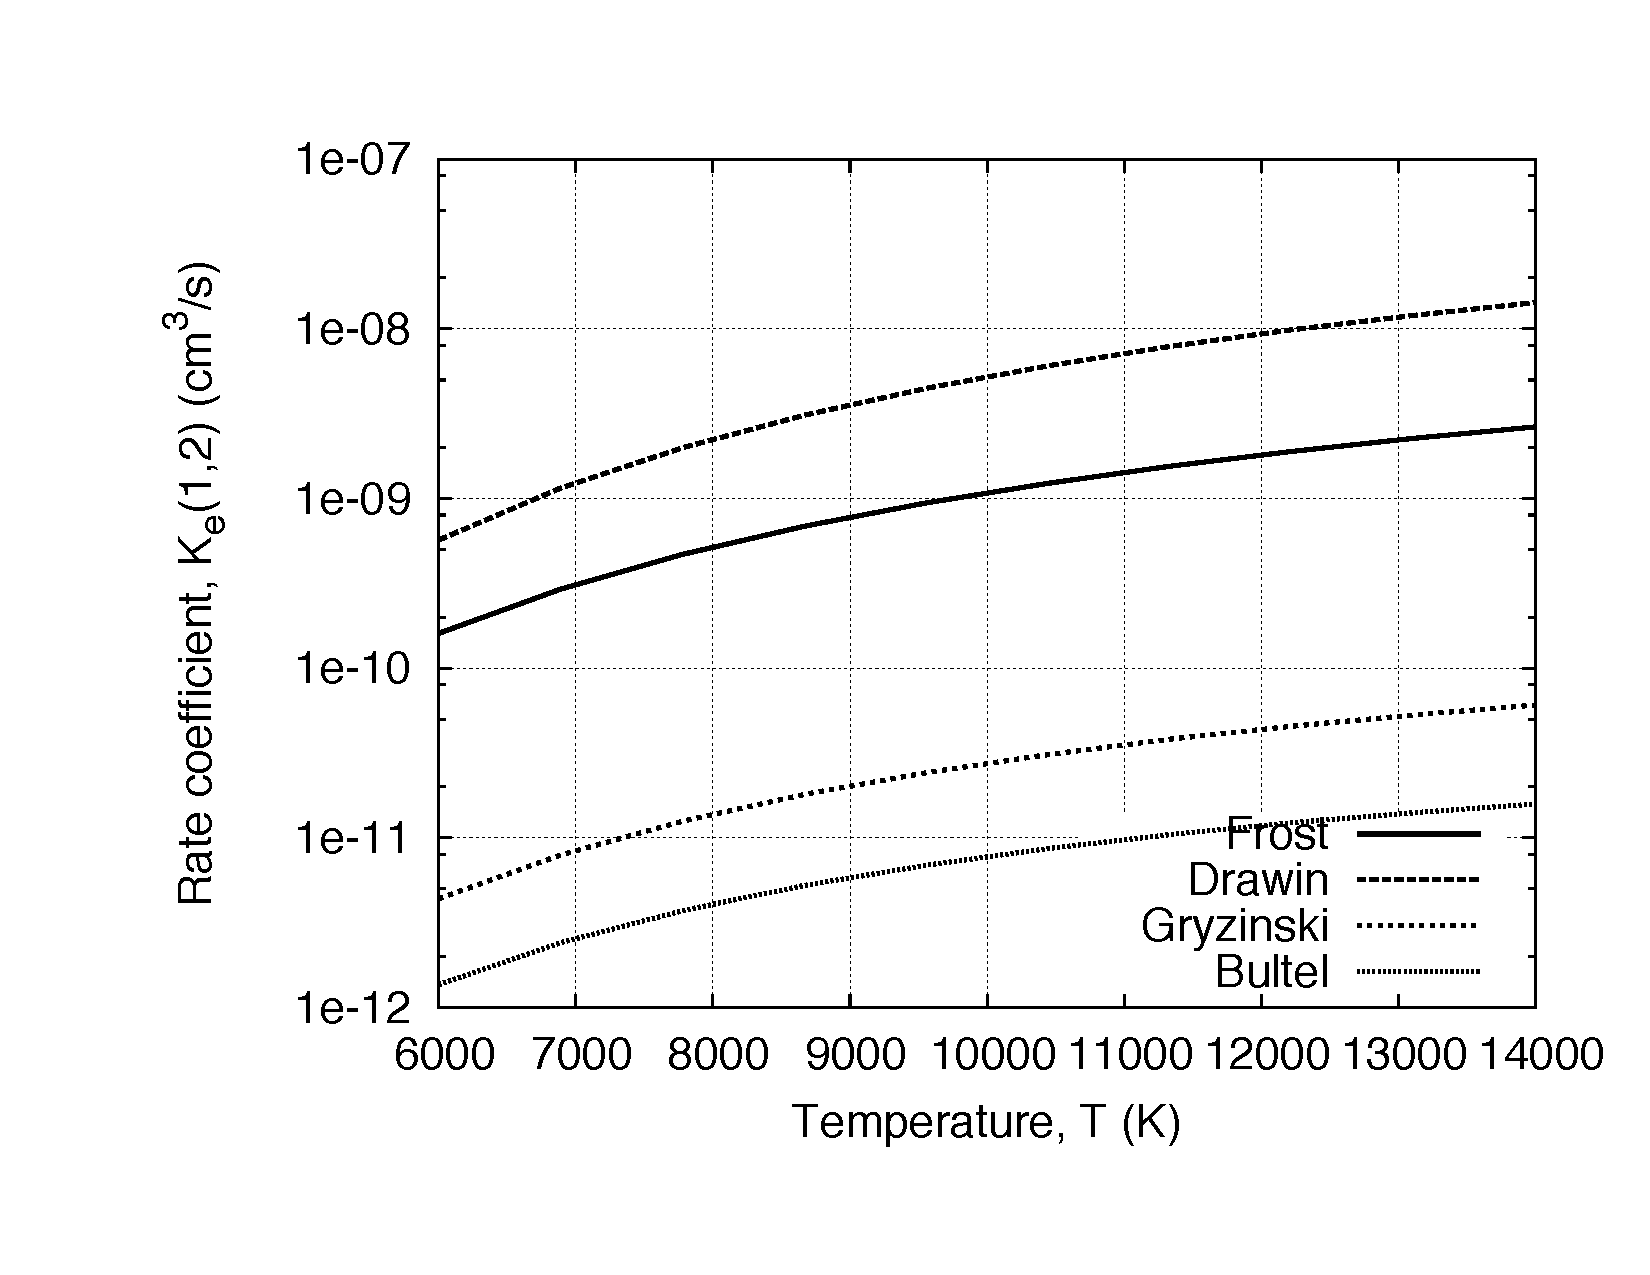
\includegraphics[width=0.48\linewidth]{collisional-radiative-modelling/figures/K_EIE_N_1_to_2.pdf} \label{fig:K_EIE_N_1_to_2}}
 \subfloat[$\Nlevone \Rightarrow \Nlevthree$ (forbidden)]{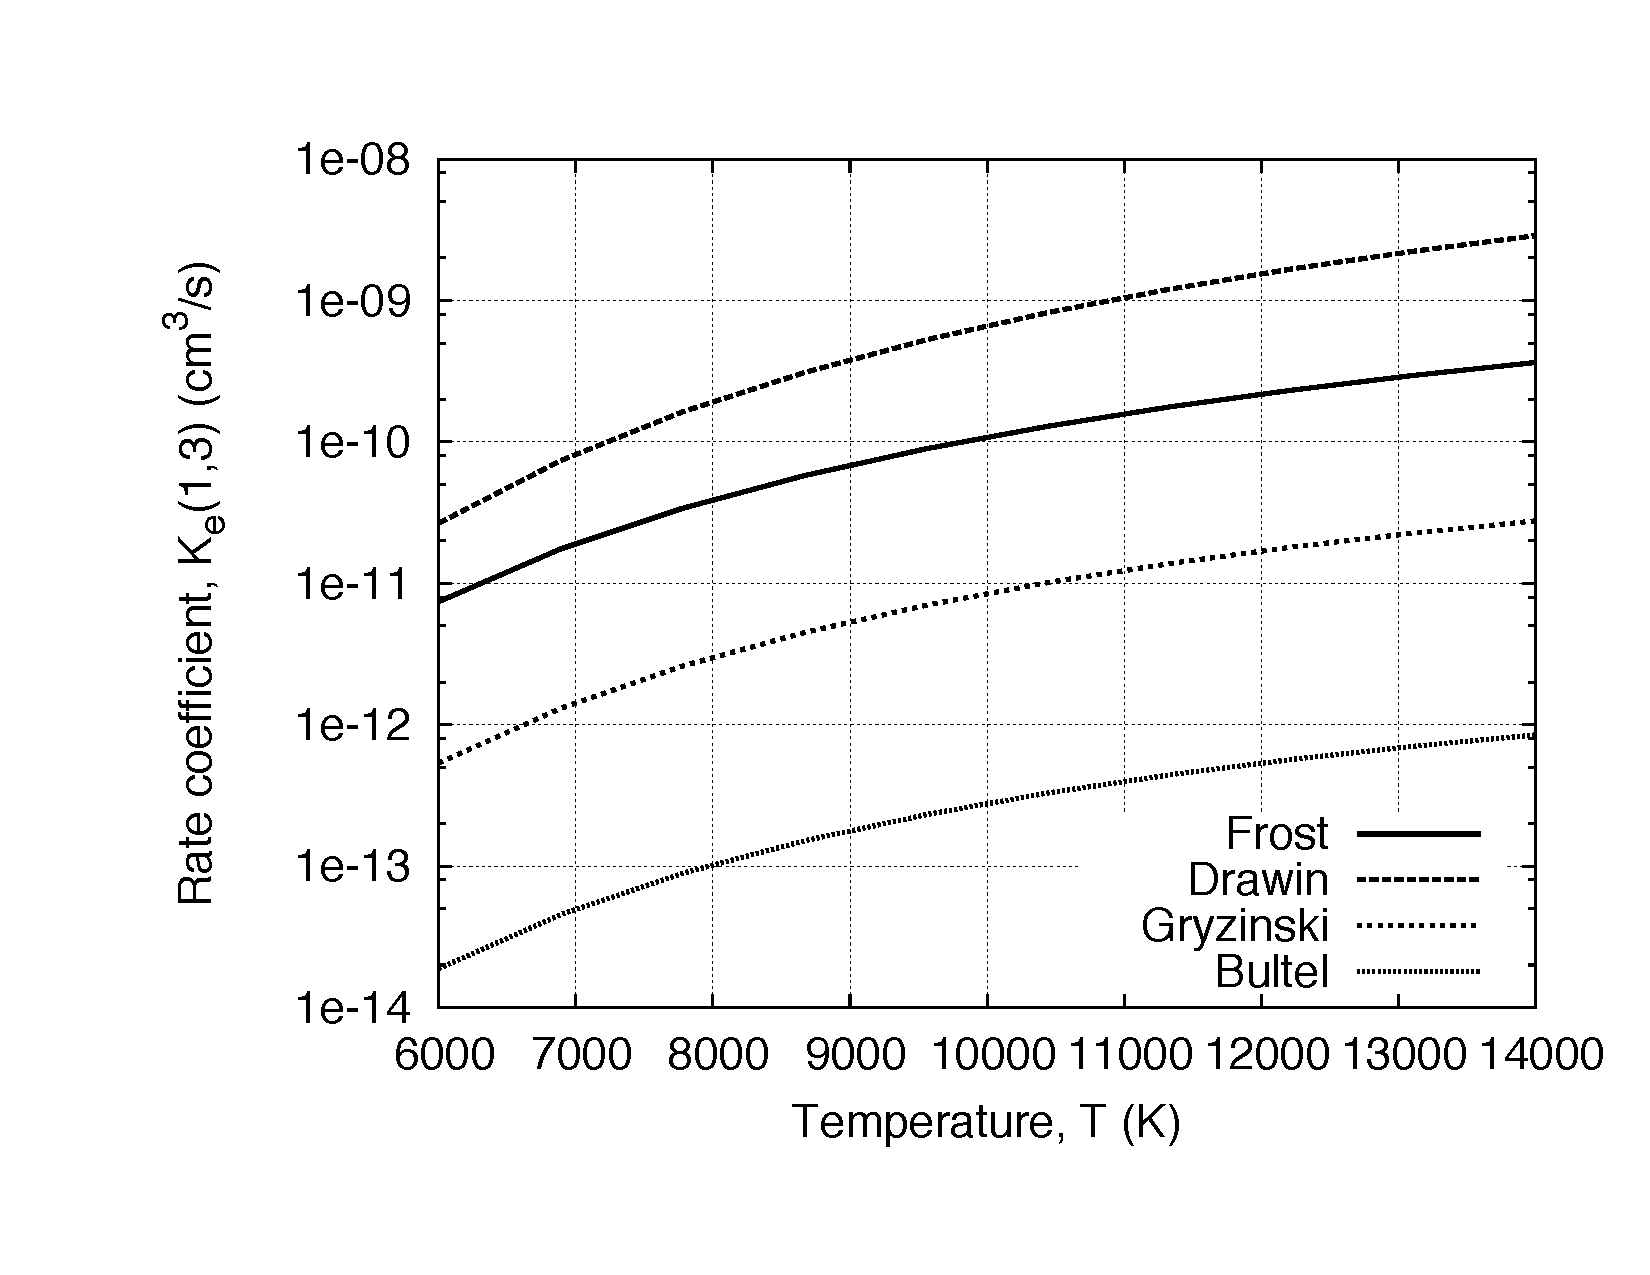
\includegraphics[width=0.48\linewidth]{collisional-radiative-modelling/figures/K_EIE_N_1_to_3.pdf} \label{fig:K_EIE_N_1_to_3}} \\
 \subfloat[$\Nlevone \Rightarrow \Nlevfive$ (forbidden)]{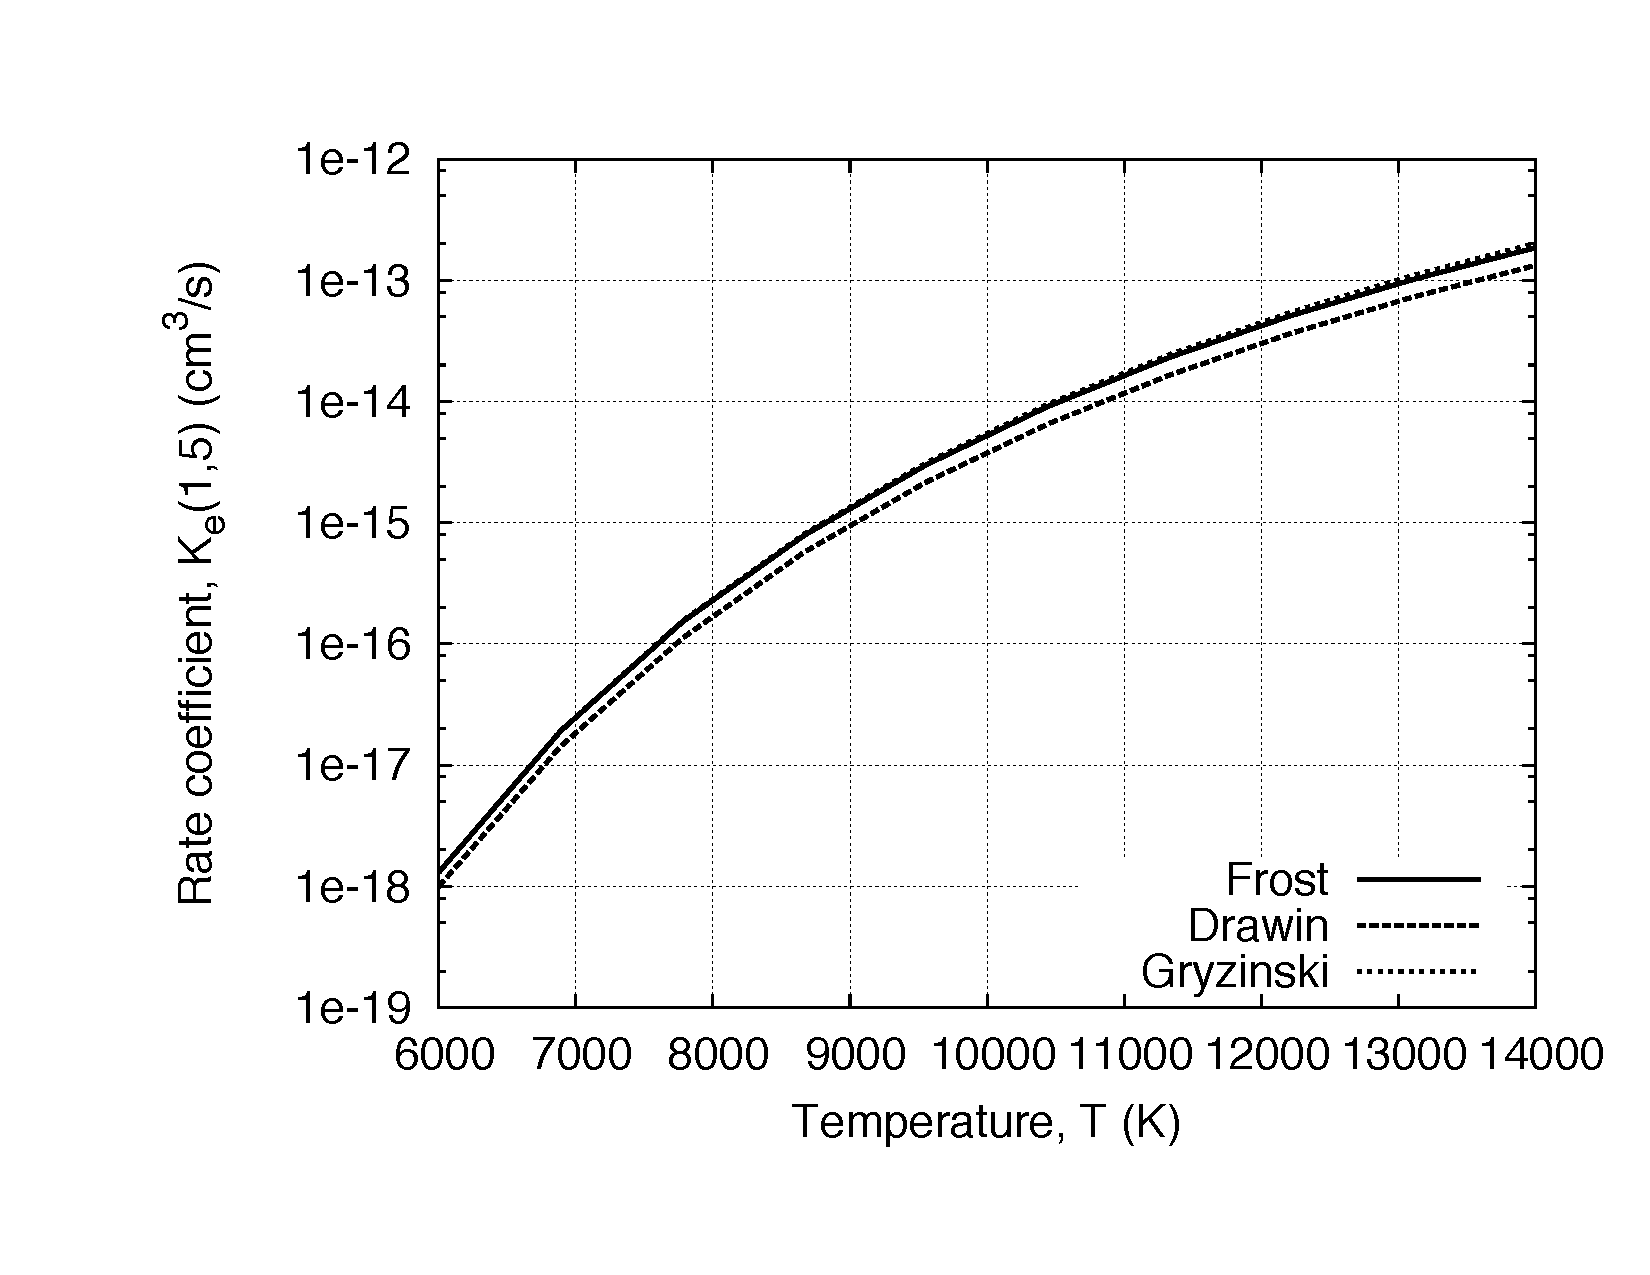
\includegraphics[width=0.48\linewidth]{collisional-radiative-modelling/figures/K_EIE_N_1_to_5.pdf} \label{fig:K_EIE_N_1_to_5}}
 \subfloat[$\Nlevtwo \Rightarrow \Nlevfive$ (allowed)]{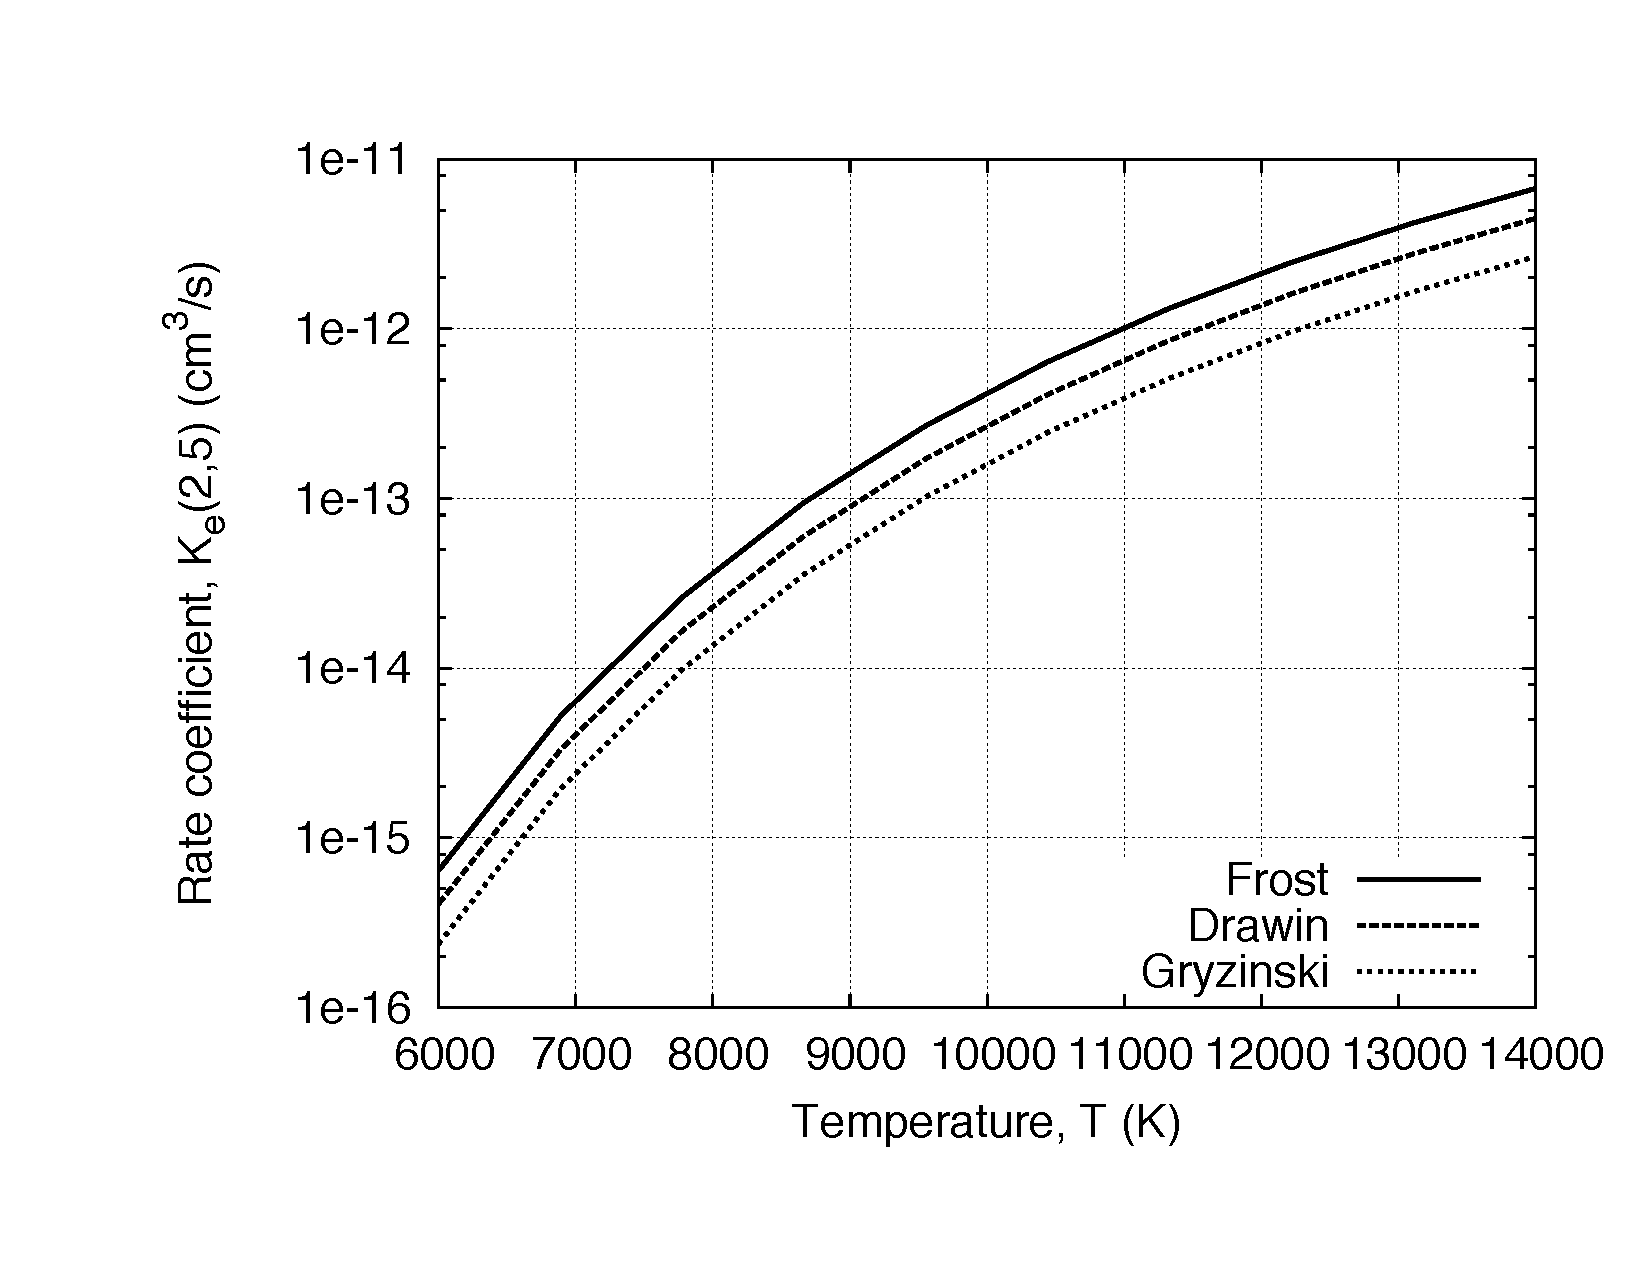
\includegraphics[width=0.48\linewidth]{collisional-radiative-modelling/figures/K_EIE_N_2_to_5.pdf} \label{fig:K_EIE_N_2_to_5}} \\
  \subfloat[$\Nlevtwo \Rightarrow \Nlevthirteen$ (allowed)]{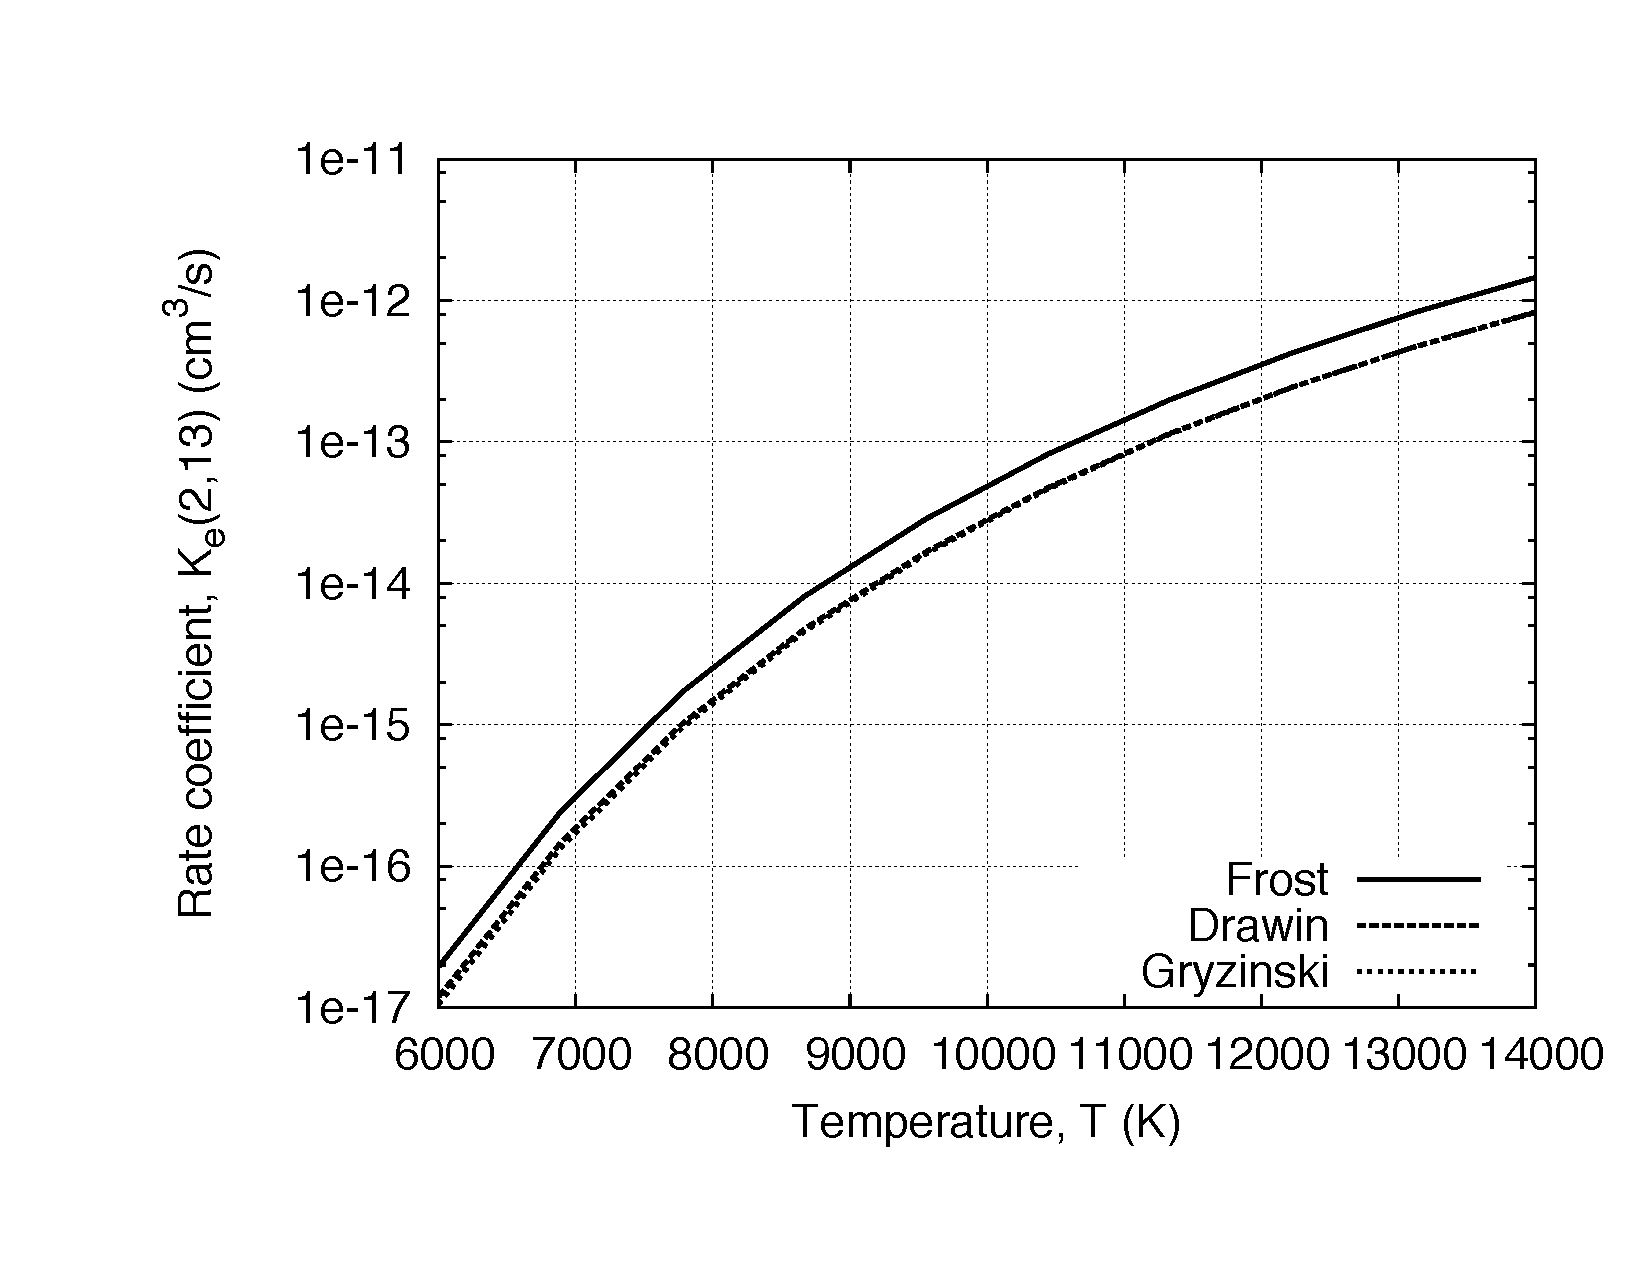
\includegraphics[width=0.48\linewidth]{collisional-radiative-modelling/figures/K_EIE_N_2_to_13.pdf} \label{fig:K_EIE_N_2_to_13}}
 \subfloat[$\Nlevthree \Rightarrow \Nlevfifteen$ (allowed)]{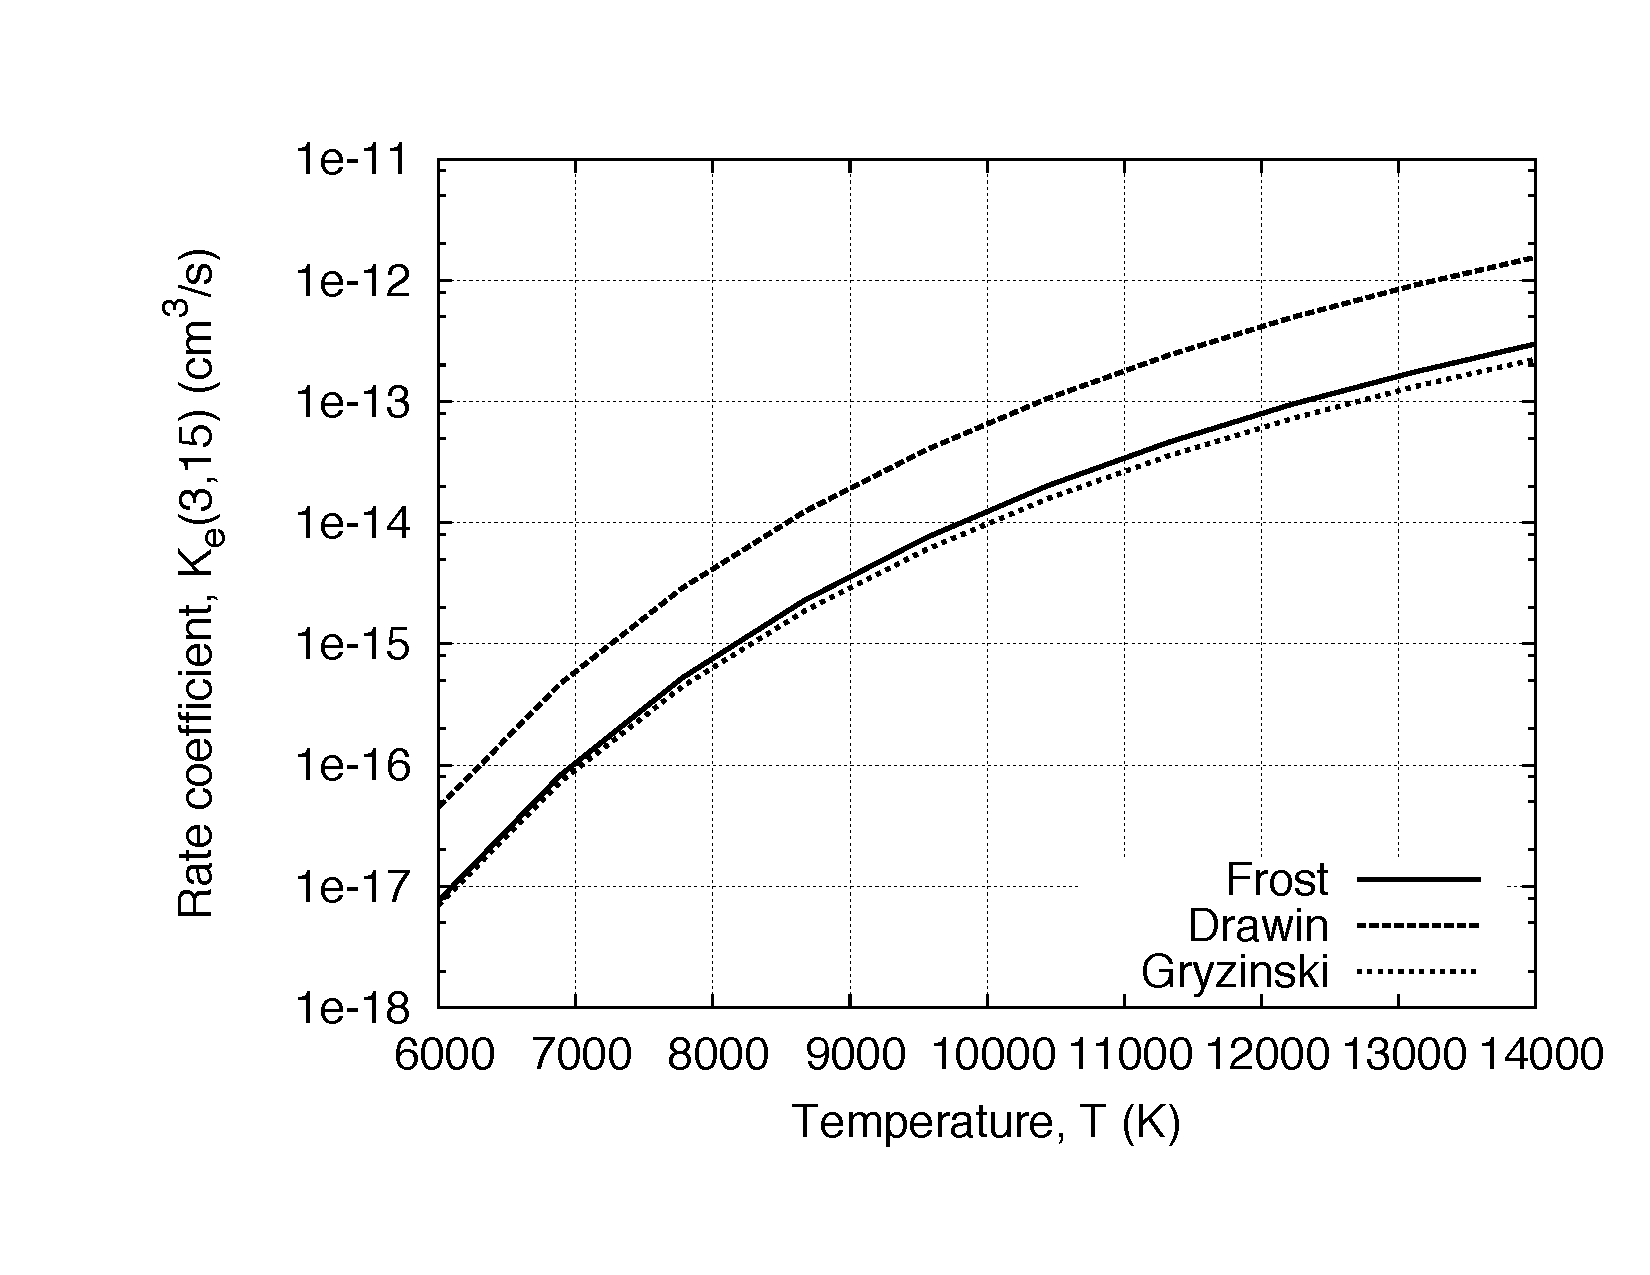
\includegraphics[width=0.48\linewidth]{collisional-radiative-modelling/figures/K_EIE_N_3_to_15.pdf} \label{fig:K_EIE_N_3_to_15}} \\
 \caption{Comparison of  electron impact excitation rate coefficients for atomic nitrogen.}
 \label{fig:K_EIE_N}
\end{figure}

\begin{figure}[h]
 \centering
 \ContinuedFloat
 \subfloat[$\Nlevone \Rightarrow \Nlevtwenty$ (forbidden)]{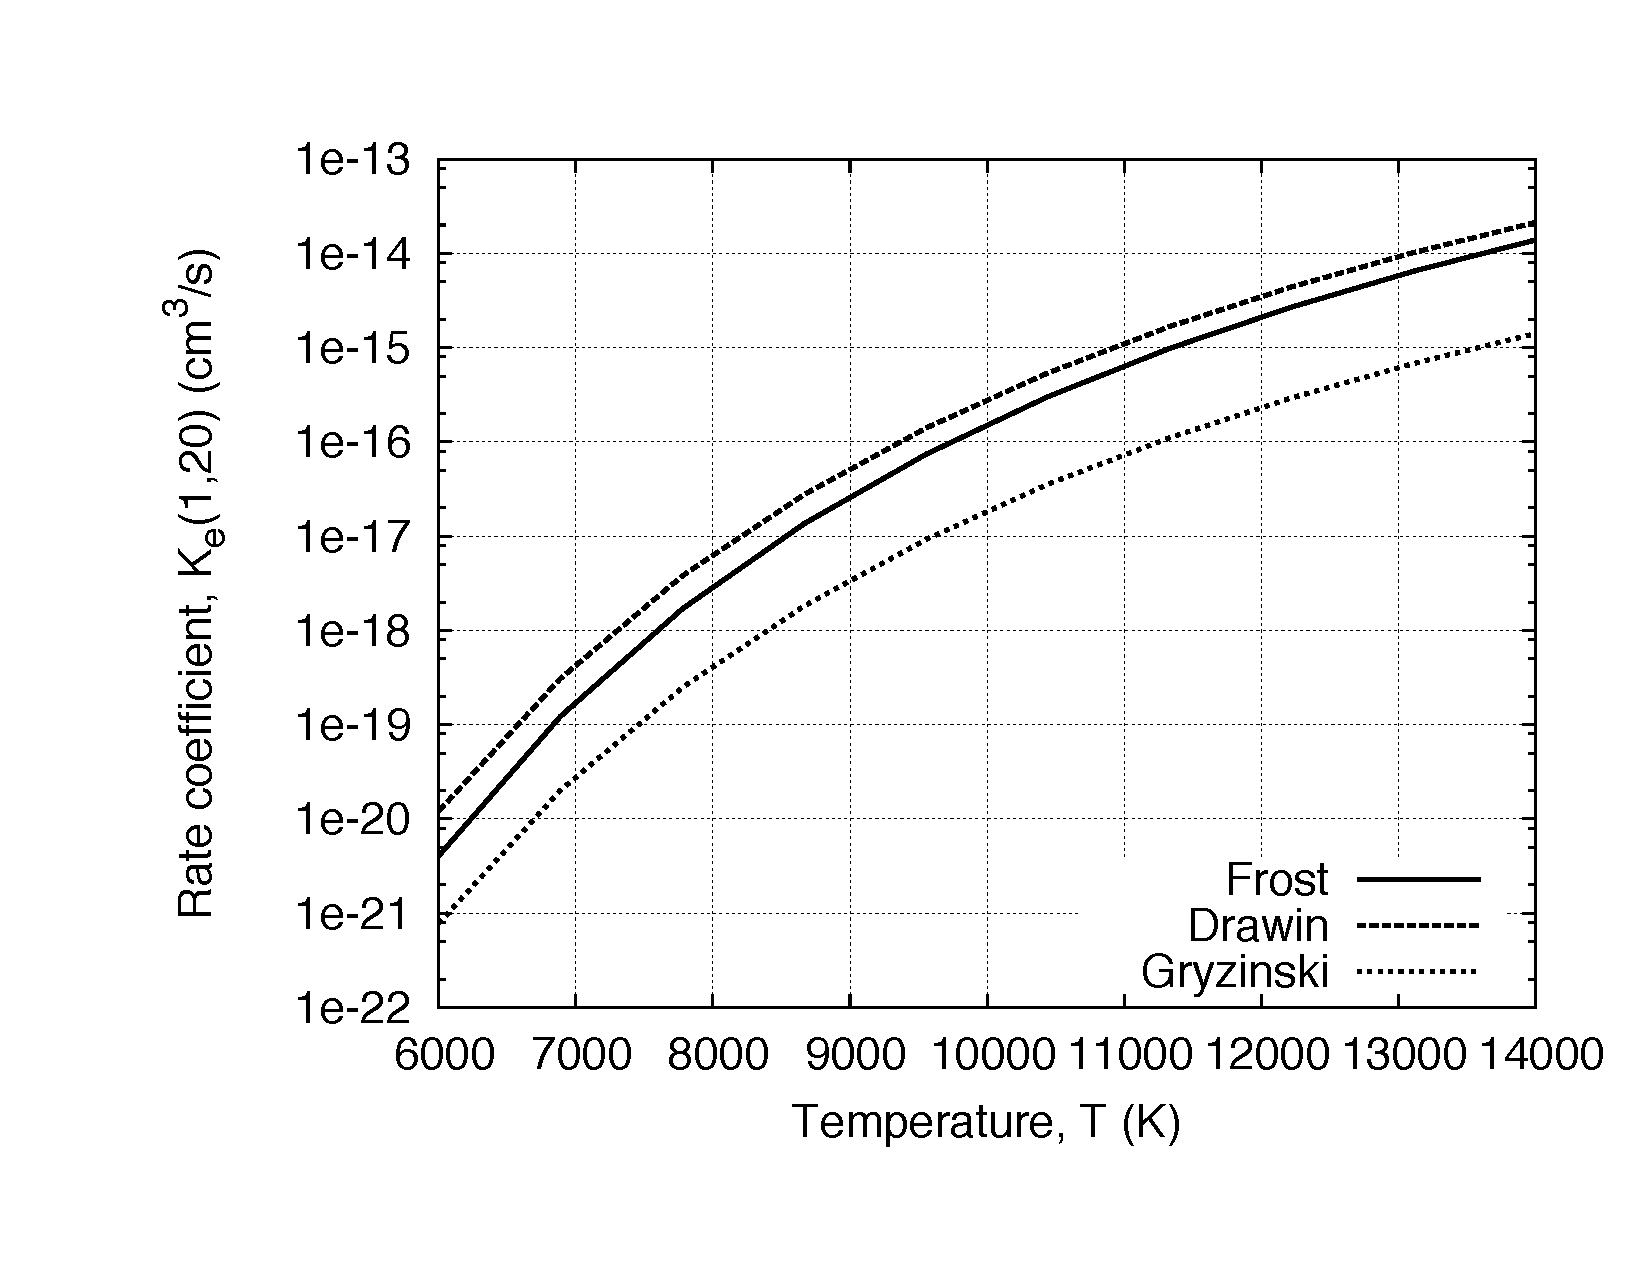
\includegraphics[width=0.48\linewidth]{collisional-radiative-modelling/figures/K_EIE_N_1_to_20.pdf} \label{fig:K_EIE_N_1_to_20}}
 \subfloat[$\Nlevthree \Rightarrow \Nlevtwenty$ (forbidden)]{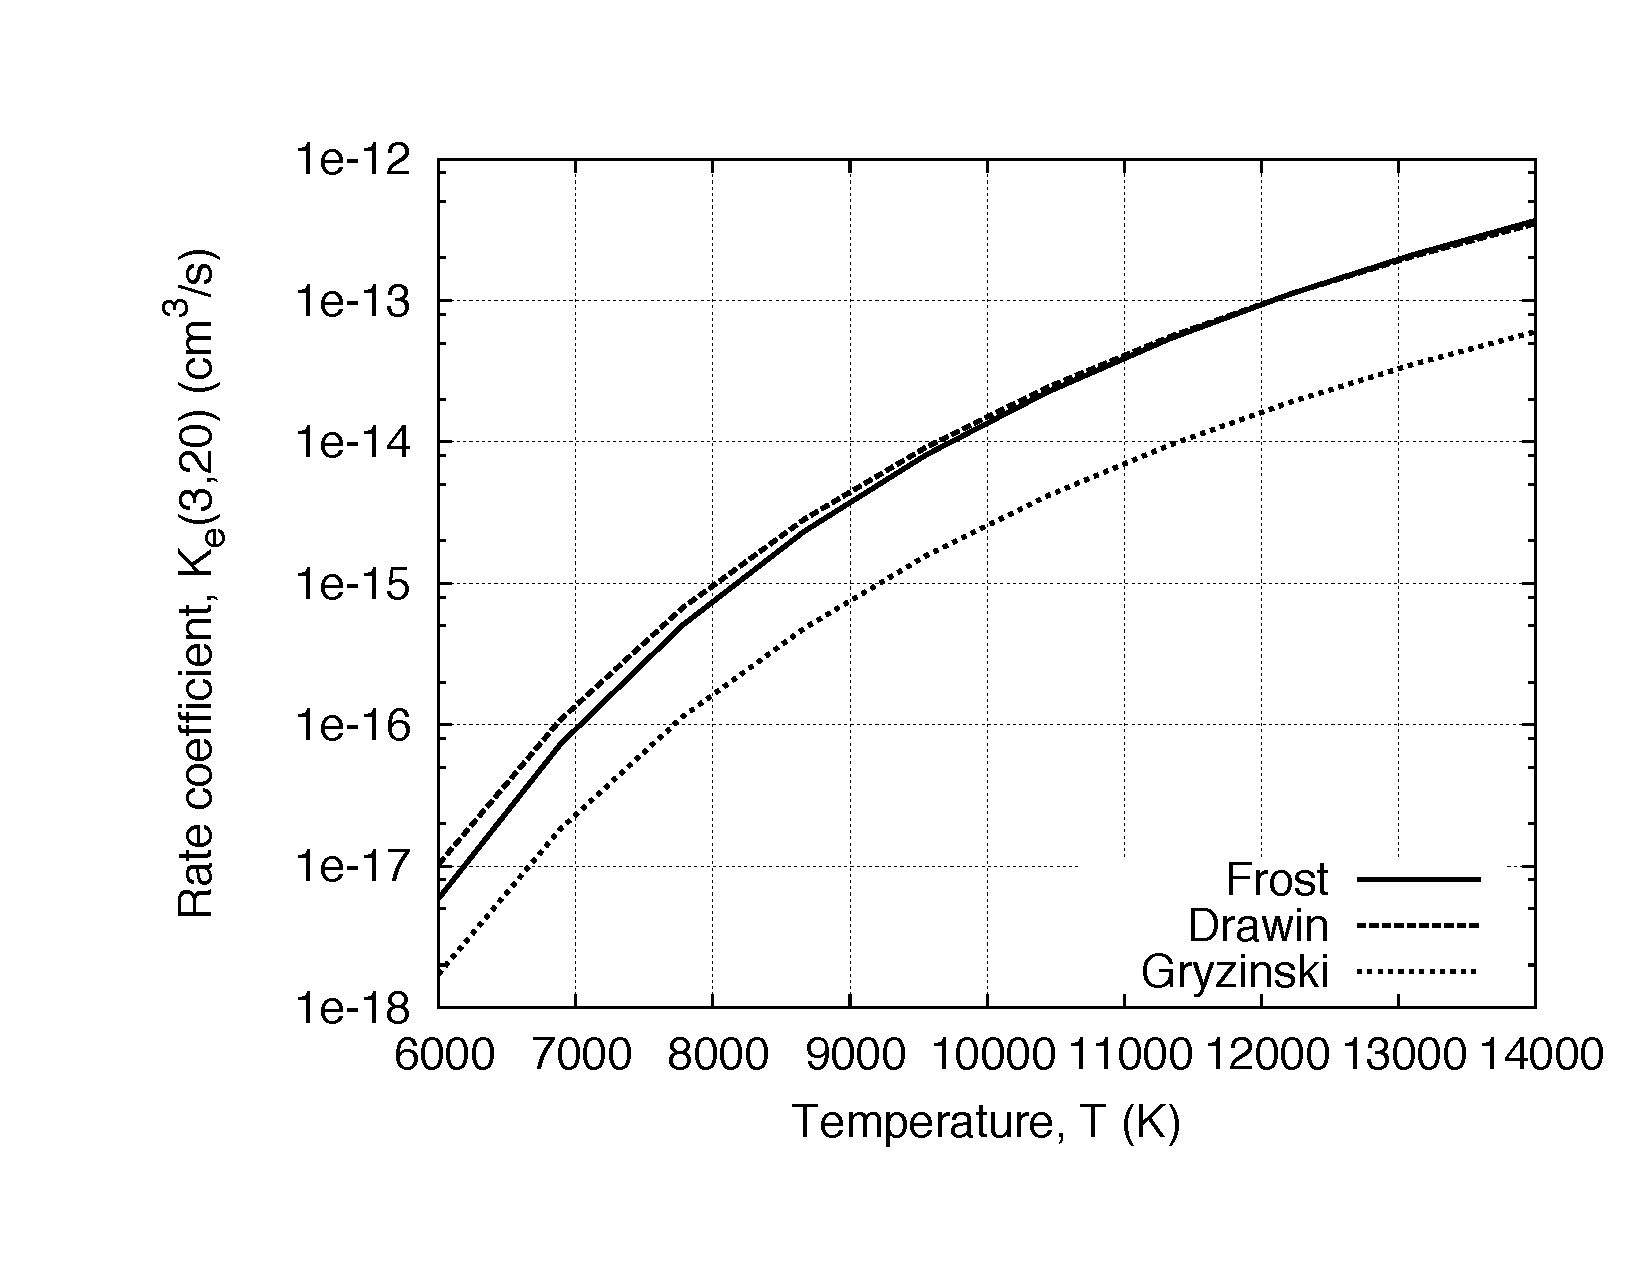
\includegraphics[width=0.48\linewidth]{collisional-radiative-modelling/figures/K_EIE_N_3_to_20.pdf} \label{fig:K_EIE_N_3_to_20}}
 \caption{\textit{(Continued)} Comparison of  electron impact excitation rate coefficients for various transitions of N.}
 \label{fig:K_EIE_N}
\end{figure}

\par

The Frost, Drawin and Gryzinski models exhibit qualitative agreement for the remaining transitions shown, Figures~\ref{fig:K_EIE_N_1_to_5} to~\ref{fig:K_EIE_N_3_to_20}.
Quantitatively, it is encouraging to observe that the data of Frost is bounded by the Gryzinski and Drawin models for almost all transitions, although there is no trend as to which forms the upper or lower bound.
For the 1-5 and 3-15 transitions in Figures~\ref{fig:K_EIE_N_1_to_5} and~\ref{fig:K_EIE_N_3_to_15}, for example, the Gryzinski data shows exceptional agreement with the calculations of Frost.
In contrast, for the 1-20 and 3-20 transitions in Figures~\ref{fig:K_EIE_N_1_to_5} and~\ref{fig:K_EIE_N_3_to_20}, the Gryzinski model subtantially underestimates the data of Frost while the Drawin model shows good agreement.
Furthermore the semi-empirical models differ by up to two orders of magnitude for some transitions.
In the present work the accurate calculations of Frost \textit{et al.}~\cite{FAS+1998} are preferred where available, with the remaining transitions described by the Gryzinski~\cite{Gryz59} model.
The decision to implement the Gryzinski model in preference to the Drawin model is based on the findings of Panesi~\cite{panesi_2008B,panesi_phd}, where the Gryzinski model gave improved agreement with the air shock tube spectroscopy experiments performed in the EAST facility.

\subsubsection{(b) Electron impact ionisation of N}

Johnston~\cite{JohnPhd} implemented the ionisation rate coefficients proposed by Kunc and Soon~\cite{KS1989} for the ground and first two excited levels of atomic nitrogen.
The rate coefficients are calculated as:

\begin{equation}
 K_e(i,c) = 1.0 \times 10^{-8} \left [ \frac{I_H}{I - E_i} \right ] \frac{Q_i}{2 l_i + 1} \text{exp} \left ( - \beta \right ) G_i \left ( \beta \right ) \label{eq:K_EII_Soon_Kunc_a}
\end{equation}

\noindent where,

\begin{equation}
 G_i ( \beta ) = \sqrt{\frac{\beta}{\beta+1}} \frac{A}{\beta + \chi} \text{ , }
\end{equation}

\noindent and, 

\begin{equation}
 \beta = \frac{I - E_i}{kT_e} \text{ . } \label{eq:K_EII_Soon_Kunc_c}
\end{equation}

\noindent The parameter $I_H$ is the ionisation energy of the hydrogen energy (Rydberg energy), $l_i$ is the angular momentum quantum number of the level $i$, $A$ and $\chi$ are fitting constants for the species and $G_i$ is level dependent angular factor.
For atomic nitrogen $A$ is equal to 27.71, $\chi$ is equal to 5.58 and $Q_i$ is equal to 3 for the ground state and $3/2$ for the first and second excited states.
This expression is a curve-fit based on the rate coefficient derived from experimentally measured electron impact ionisation cross sections for the ground state of N.

\par

Panesi~\cite{panesi_phd} implemented the ionisation rate coefficients presented by Bultel \textit{et al.}~\cite{BBB+2006}, which were obtained from the compilation of Tawara and Kato~\cite{TK1999} and the combined binary-encounter Bethe (BEB) and scaled plane-wave Born (PWB) calculations of Kim and Desclaux~\cite{KD2002}.
The rates for the ground and first two excited states of N were presented as generalised Arrhenius curve-fits in the temperature range 2,000 $\leq T_e \leq$ 10,000\,K.

\par

Figure~\ref{fig:K_EII_N} compares the electron impact ionisation rate coefficient for various transitions of N.
As was observed for the electron impact excitation rates, the Bultel generalised Arrhenius expressions substantially underestimates the rates of all other models --- by as much as six orders of magnitude for ionisation of the metastable states, Figures~\ref{fig:K_EII_N_2} and~\ref{fig:K_EII_N_3}.
It is unclear how the Bultel rates are able to be valid in the quoted 2,000 $\leq T_e \leq$ 10,000\,K temperature range when the minimum electron temperature considered in the calculations of Kim and Desclaux~\cite{KD2002} is 12\,eV ($\approx$ 140,000\,K).
The Drawin models implemented by Johnston~\cite{JohnPhd} and Panesi~\cite{panesi_phd} bound the experimentally fitted model of Soon and Kunc~\cite{SK1990}, with Panesi's implementation being in closer agreement.
Although the difference between the two Drawin models decreases as ionisation from higher levels and low electron temperatures is considered (see Figure~\ref{fig:K_EII_N_13}), Johnston's implementation is between approximately 2 and 100 times smaller for all levels.
Therefore in the present work the electron impact ionisation coefficients of Soon and Kunc~\cite{SK1990} are preferred for the first three levels, while the Drawin model implemented by Panesi~\cite{JohnPhd} is used for the remaining levels.

\begin{figure}[th]
 \centering
 \subfloat[$\text{N } \Nlevone \Rightarrow \text{N}^+$]{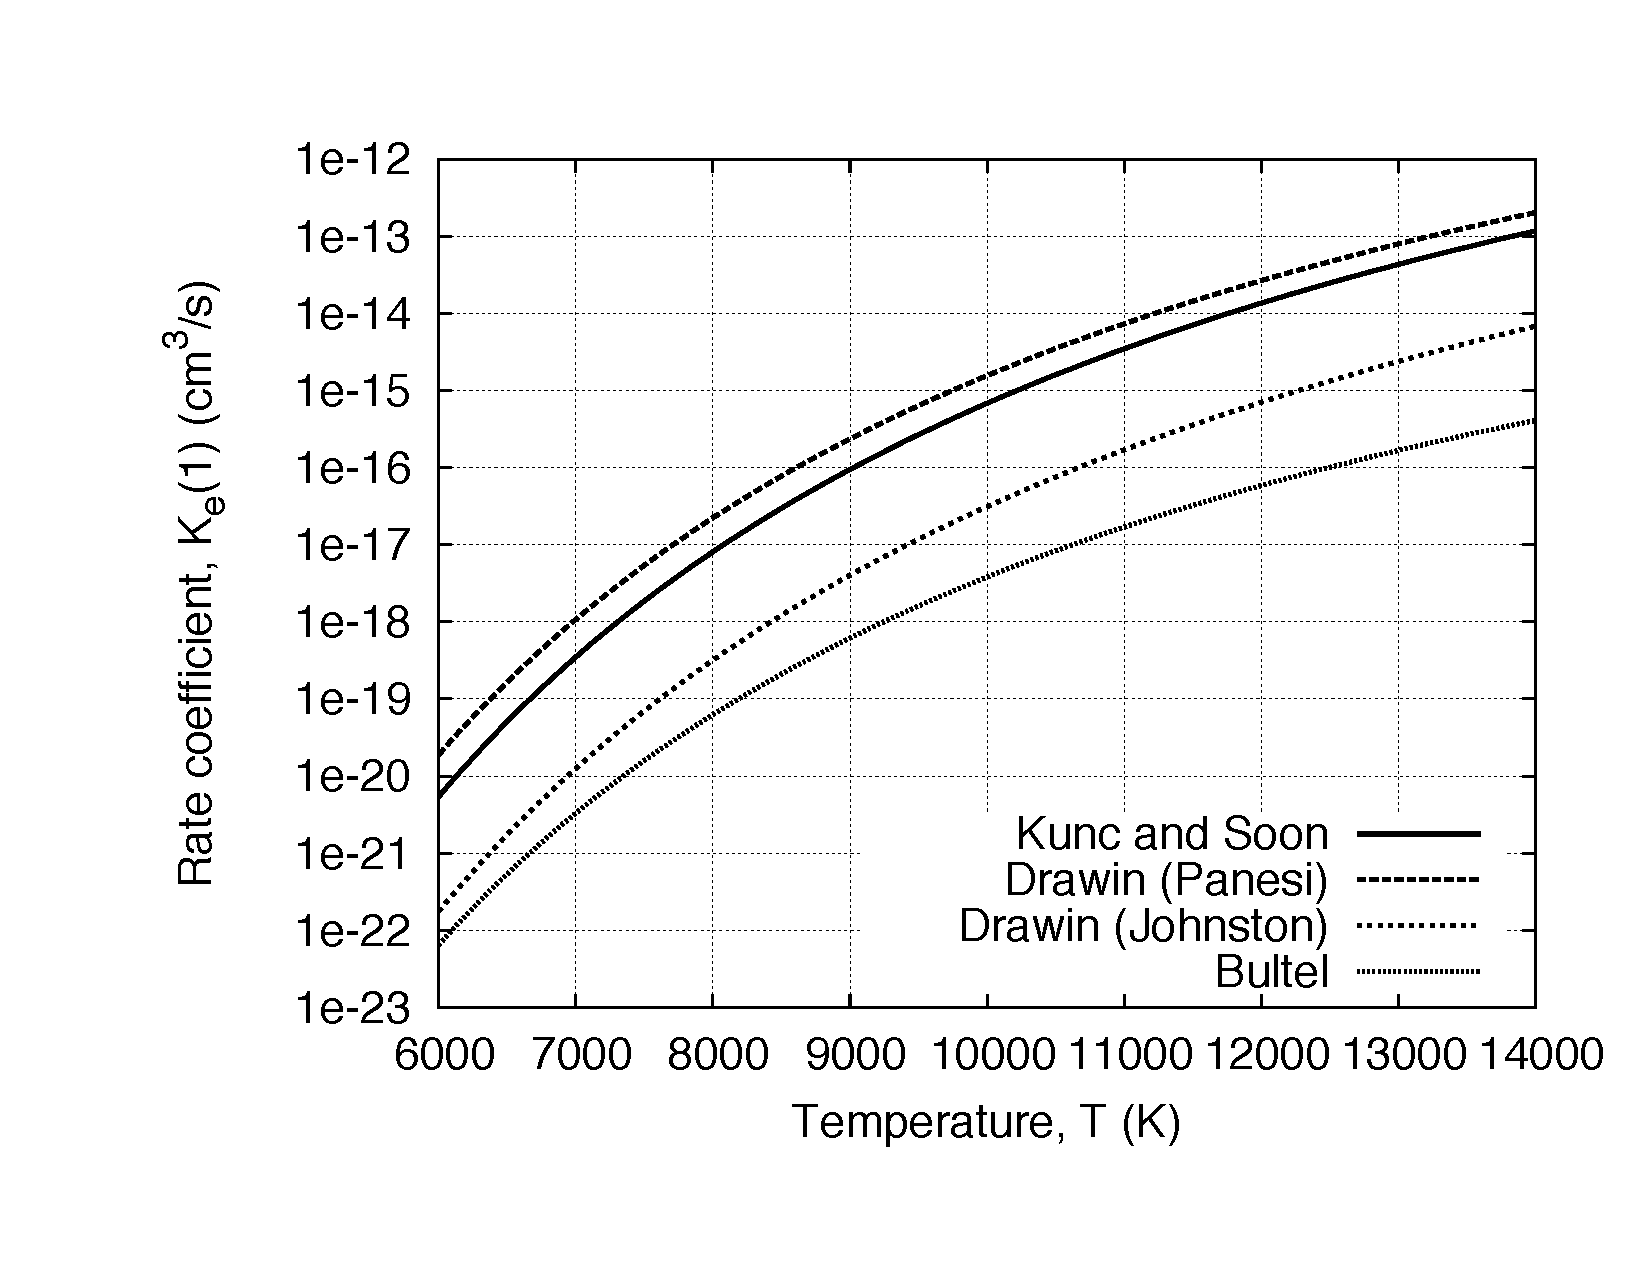
\includegraphics[width=0.48\linewidth]{collisional-radiative-modelling/figures/K_EII_N_1.pdf} \label{fig:K_EII_N_1}}
 \subfloat[$\text{N } \Nlevtwo \Rightarrow \text{N}^+$]{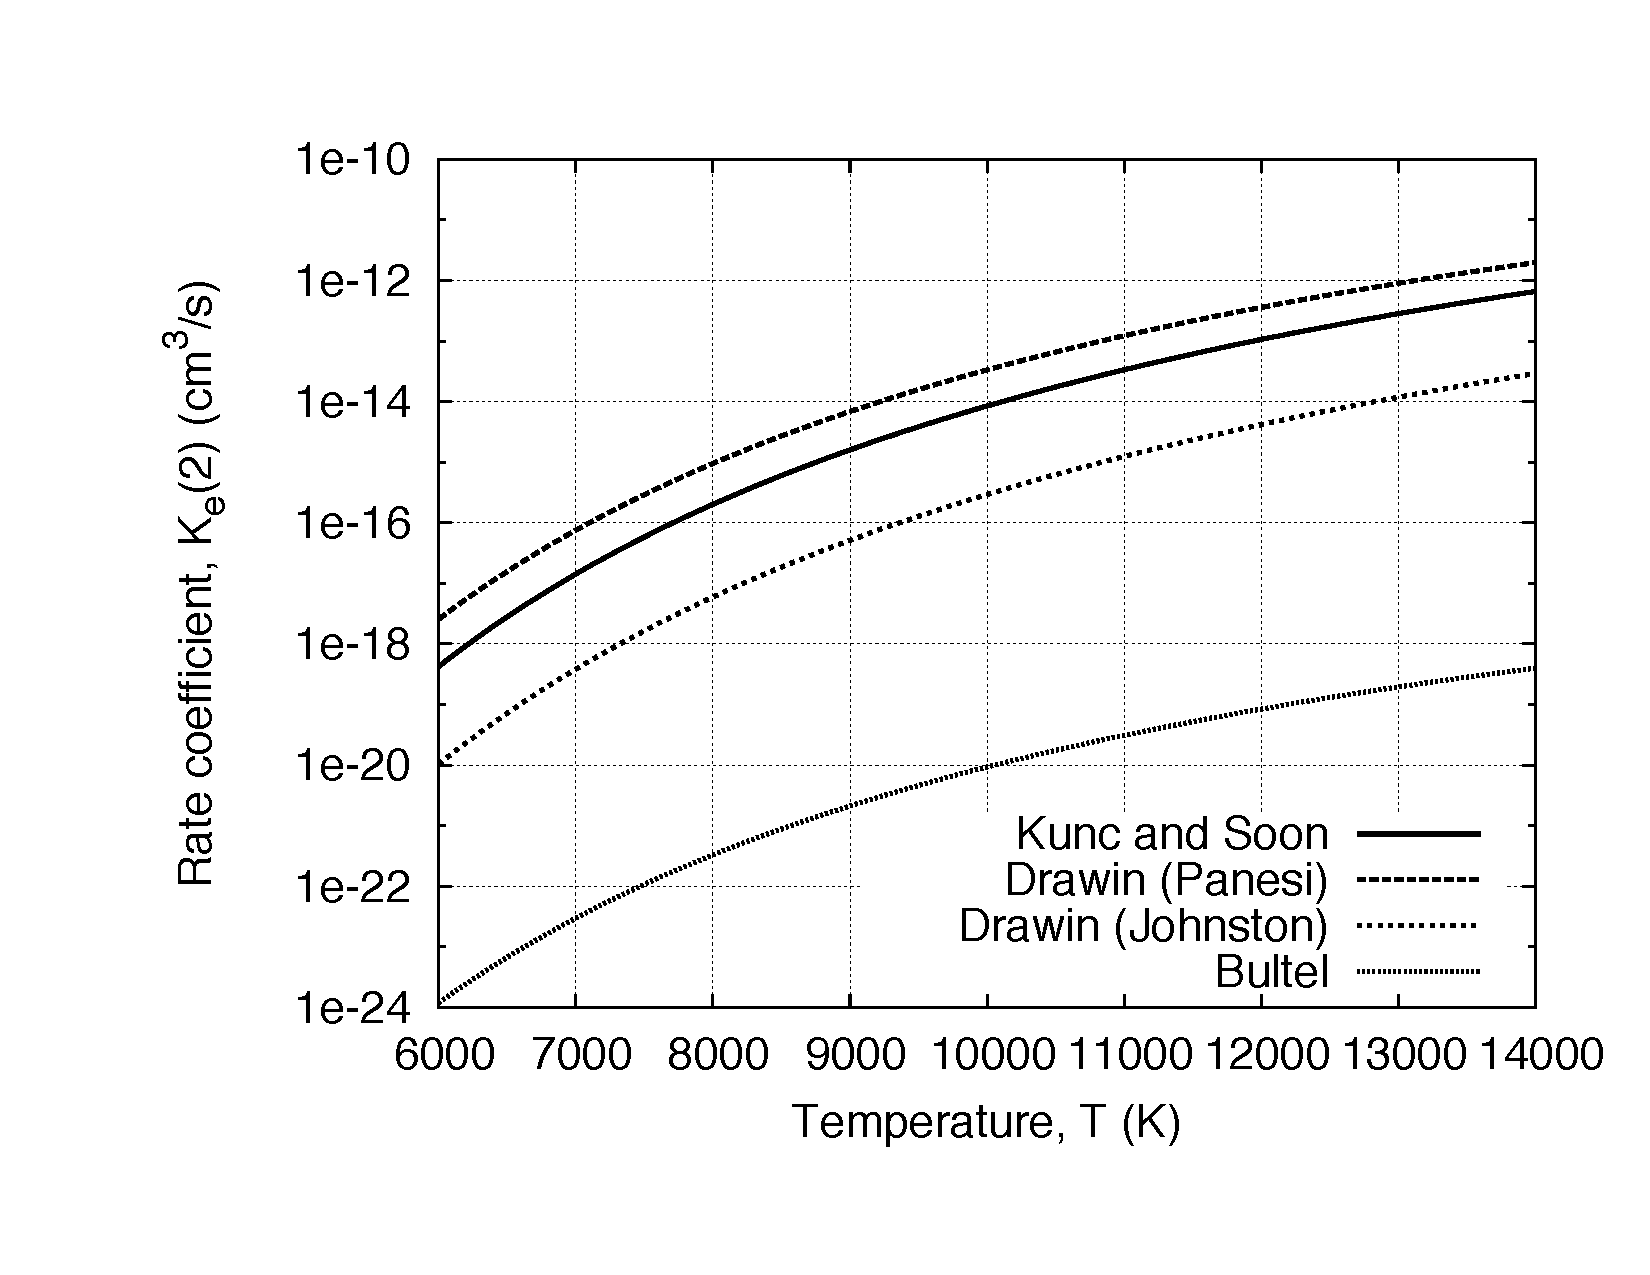
\includegraphics[width=0.48\linewidth]{collisional-radiative-modelling/figures/K_EII_N_2.pdf} \label{fig:K_EII_N_2}} \\
 \subfloat[$\text{N } \Nlevthree \Rightarrow \text{N}^+$]{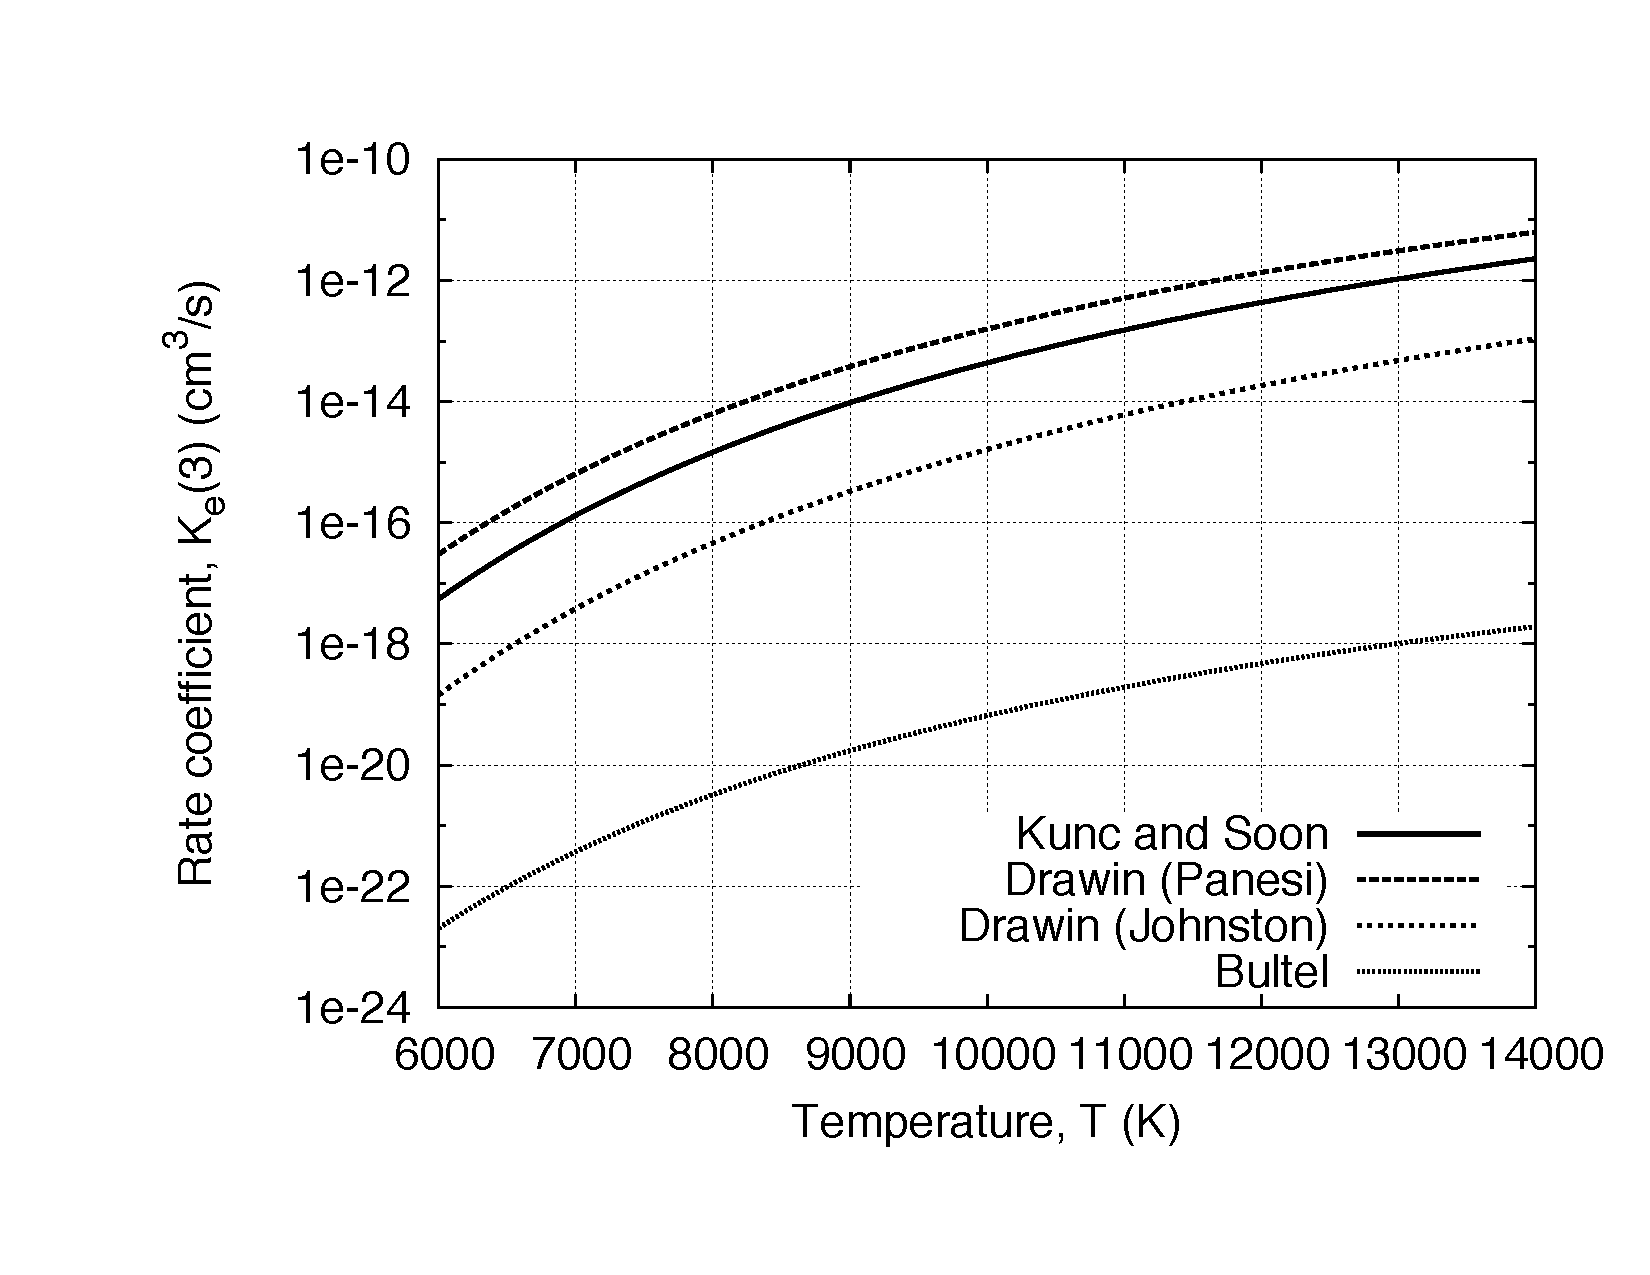
\includegraphics[width=0.48\linewidth]{collisional-radiative-modelling/figures/K_EII_N_3.pdf} \label{fig:K_EII_N_3}}
 \subfloat[$\text{N } \Nlevthirteen \Rightarrow \text{N}^+$]{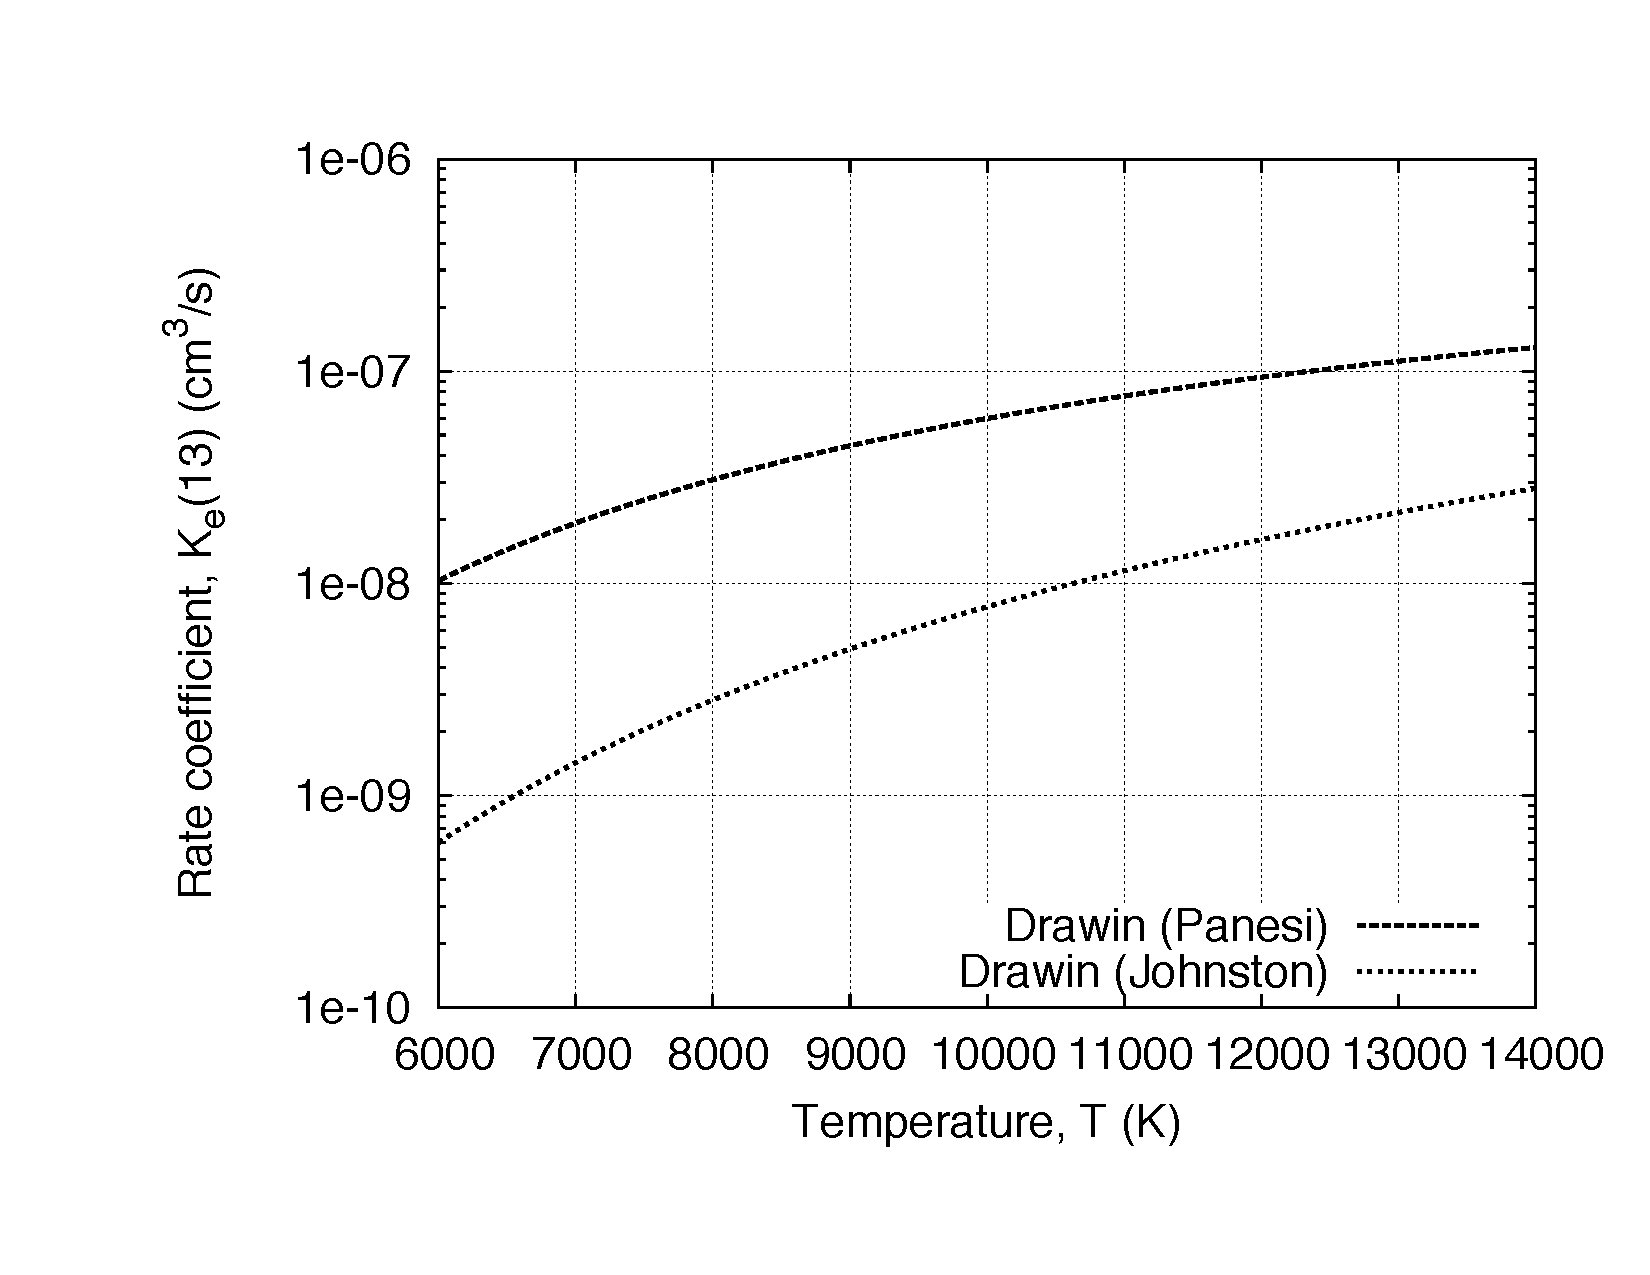
\includegraphics[width=0.48\linewidth]{collisional-radiative-modelling/figures/K_EII_N_13.pdf} \label{fig:K_EII_N_13}}
 \caption{Comparison of electron impact ionisation rate coefficients for atomic nitrogen.}
 \label{fig:K_EII_N}
\end{figure}

\subsubsection{(a) Electron impact excitation of O}

Zatsarinny and Tayal~\cite{ZT2003} calculated electron impact excitation rates for the ground and first two excited states of atomic oxygen using a $B$-spline $R$-matrix approach.
The forward rate coefficients for the Zatsarinny and Tayal model are calculated as:

\begin{equation}
K_e(i,j) = \frac{8.629 \times 10^{-6}}{g_i \sqrt{T_e}} \gamma_{ij}(T_e) \text{exp} \left ( \frac{-\Delta E_{ij}}{k T_e} \right ) % cm**3 / s
\end{equation}

\noindent where the dimensionless effective collision strength $\gamma_{ij}$ is tabulated as a function of the free electron temperature in Reference~\cite{ZT2003}.
The Zatsarinny and Tayal~\cite{ZT2003} data was the preferred source of accurate atomic oxygen electron impact excitation rates in the collisional-radiative model proposed by Johnston~\cite{JohnPhd}.

\par

Panesi~\cite{panesi_phd} implemented the electron impact excitation rate coefficients presented by Bultel \textit{et al.}~\cite{BBB+2006} which are based on the literature survey of Itikawa and Ichimura~\cite{II1990}.
Electron impact excitation rate coefficients for transitions from the ground state to the two metastable states of atomic oxygen were presented as generalised Arrhenius curve-fits in the temperature range 2,000 $\leq T_e \leq$ 10,000\,K.

\par

Figure~\ref{fig:K_EIE_O} compares the electron impact excitation rate coefficient for various transitions of atomic oxygen for which Zatsarinny and Tayal~\cite{ZT2003} present data.
For the transitions to the metastable states, Figures~\ref{fig:K_EIE_O_1_to_2} and~\ref{fig:K_EIE_O_1_to_3}, the Drawin and Gryzinski models substantially overestimated the theoretical calculations of Zatsarinny and Tayal.
Such a discrepency is to be expected for these inner core transitions due to the hydrogenic assumptions of the Drawin and Gryzinski models.
The accuracy of the Bultel rates is questionable as they more closely follow the approximate models rather than the theoretical calculations of Zatsarinny and Tayal.
Although the $B$-spline $R$-matrix calculations of Zatsarinny and Tayal are bounded by the semi-empirical models for most transitions, for some forbidden transitions such as $2-5$ and $3-7$, Figures~\ref{fig:K_EIE_O_2_to_5} and~\ref{fig:K_EIE_O_3_to_7}, the semi-empirical models underestimate the theoretical rates by at least an order of magnitude for the temperature range considered.
Some some transitions such as 1-16 and 1-17, Figures~\ref{fig:K_EIE_O_1_to_16} and~\ref{fig:K_EIE_O_1_to_17}, the Gryzinski model closely matches the Zatsarinny and Tayal calculations, whilst for others such as 1-20, Figure~\ref{fig:K_EIE_O_1_to_20}, the Drawin model shows exceptional agreement.
The Drawin and Gryzinski models show considerable variability in their relative magnitudes, being within a factor of 2 of each other for some transitions and in excess of $10^4$ for some transitions to high lying states (\textit{e.g.} Figures~\ref{fig:K_EIE_O_1_to_20} and~\ref{fig:K_EIE_O_2_to_20}).
As for atomic nitrogen, we must again bear in mind that Panesi~\cite{panesi_2008B,panesi_phd} found improved agreement with experiment when using the Gryzinski model.
Therefore in the present work the Zatsarinny and Tayal~\cite{ZT2003} rate coefficients are preferred where available, while the Gryzinski~\cite{Gryz59} model is applied to the remaining transitions.

\begin{figure}[p]
 \centering
 \subfloat[$\Olevone \Rightarrow \Olevtwo$ (Forbidden)]{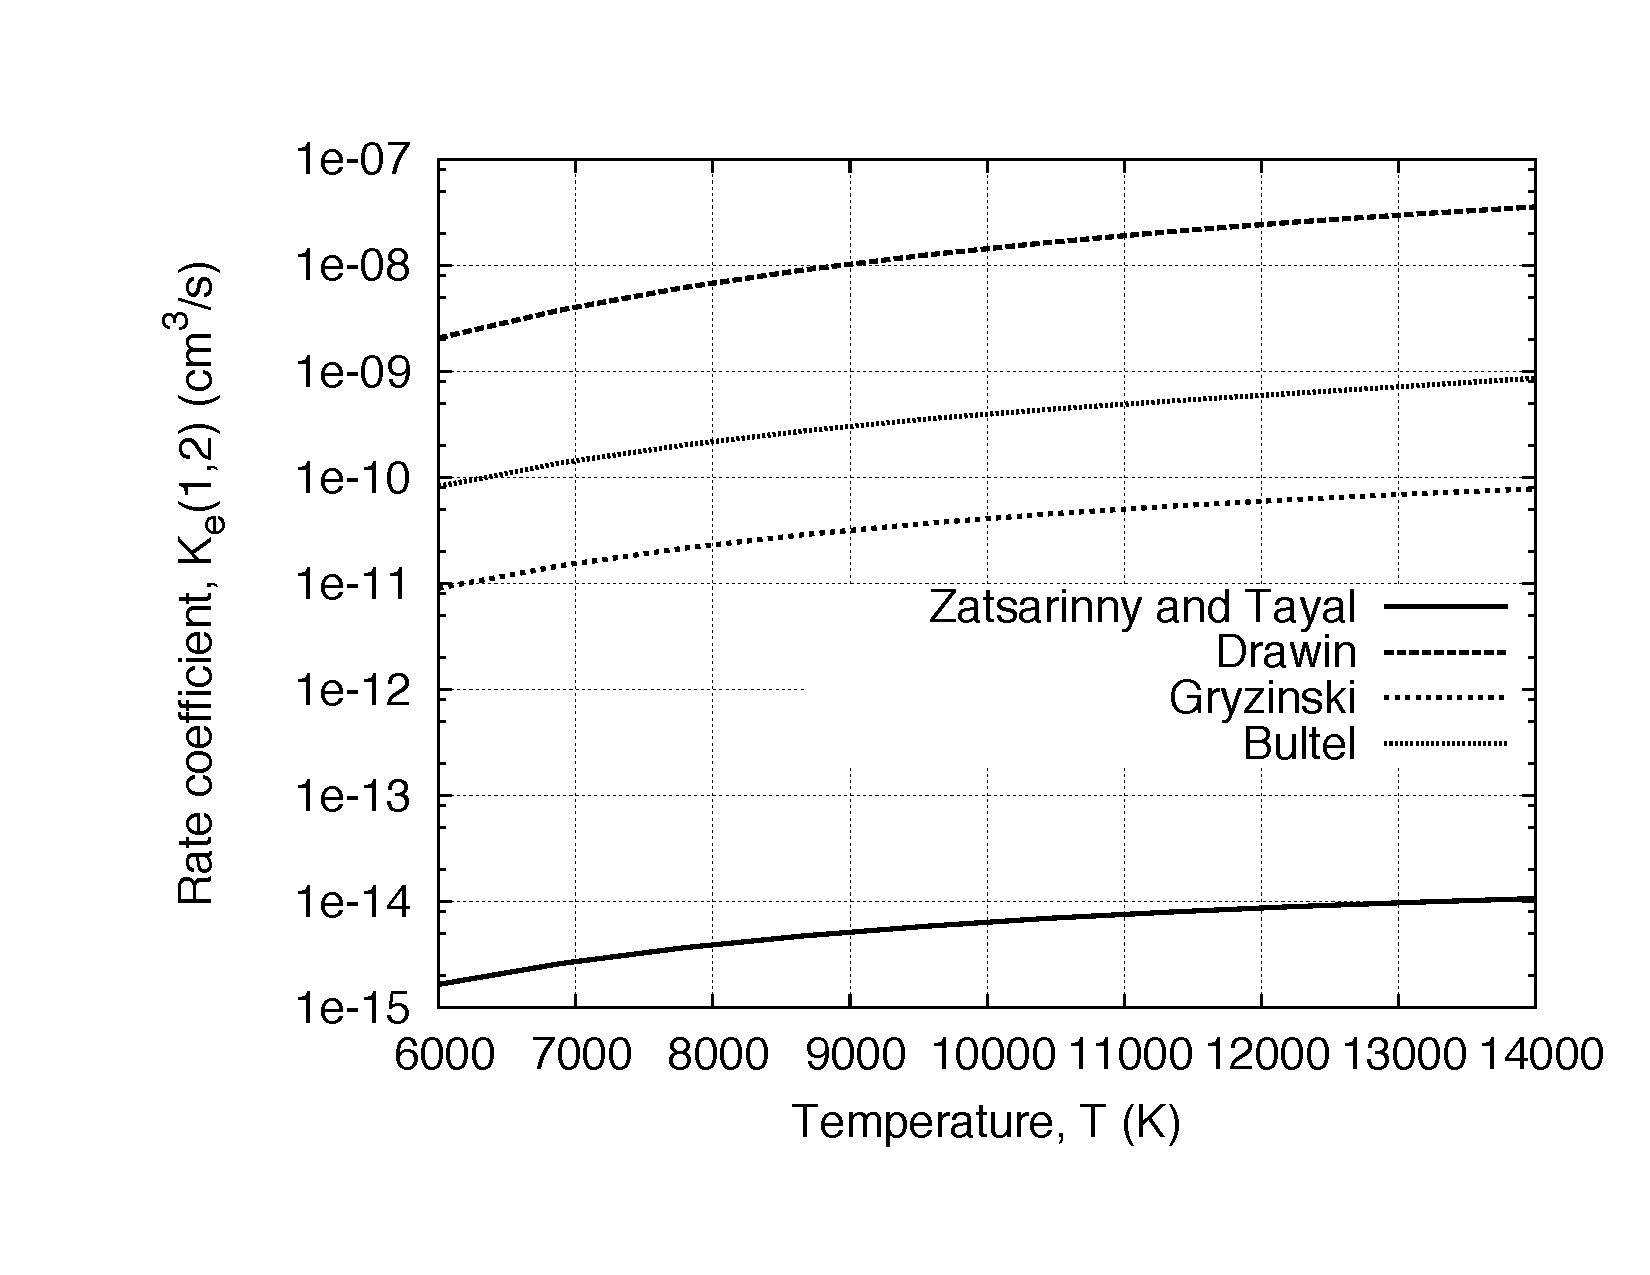
\includegraphics[width=0.48\linewidth]{collisional-radiative-modelling/figures/K_EIE_O_1_to_2.pdf} \label{fig:K_EIE_O_1_to_2}}
 \subfloat[$\Olevone \Rightarrow \Olevthree$ (Forbidden)]{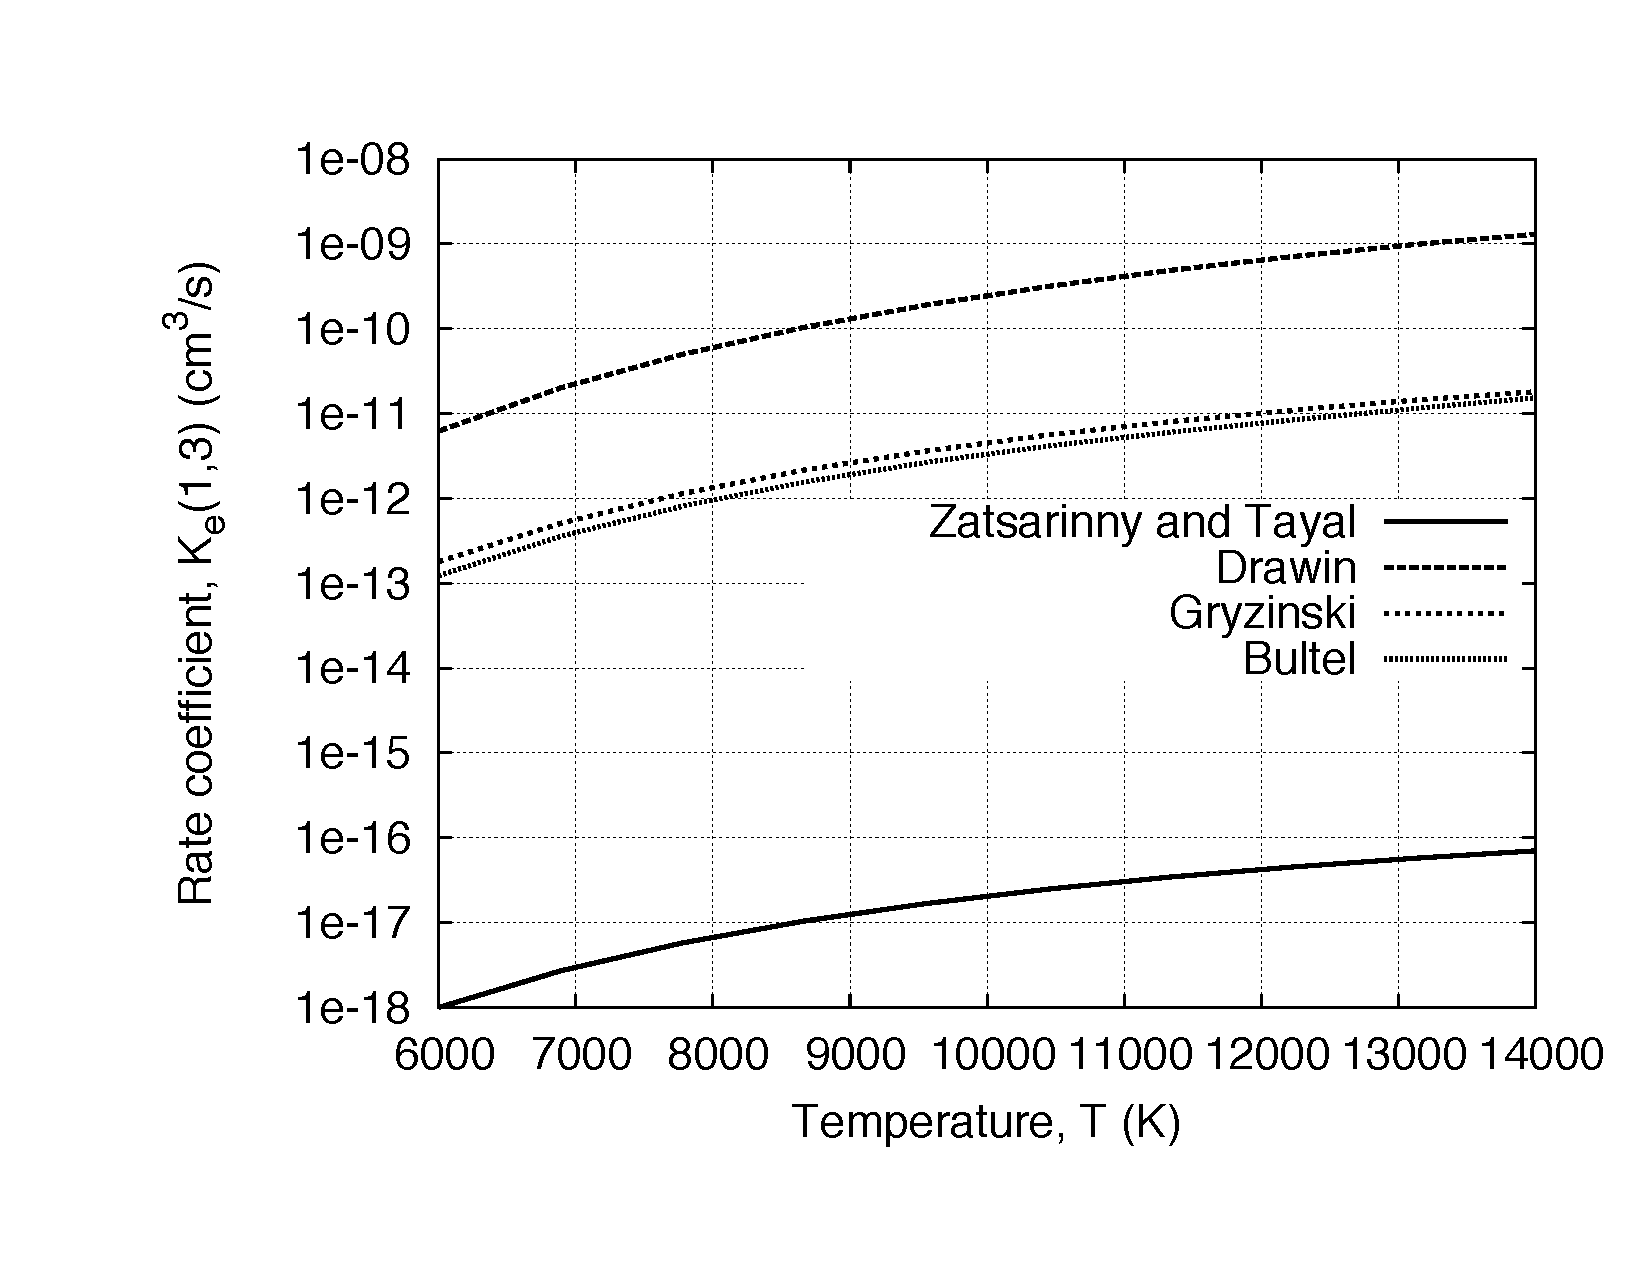
\includegraphics[width=0.48\linewidth]{collisional-radiative-modelling/figures/K_EIE_O_1_to_3.pdf} \label{fig:K_EIE_O_1_to_3}} \\
 \subfloat[$\Olevone \Rightarrow \Olevfive$ (Allowed)]{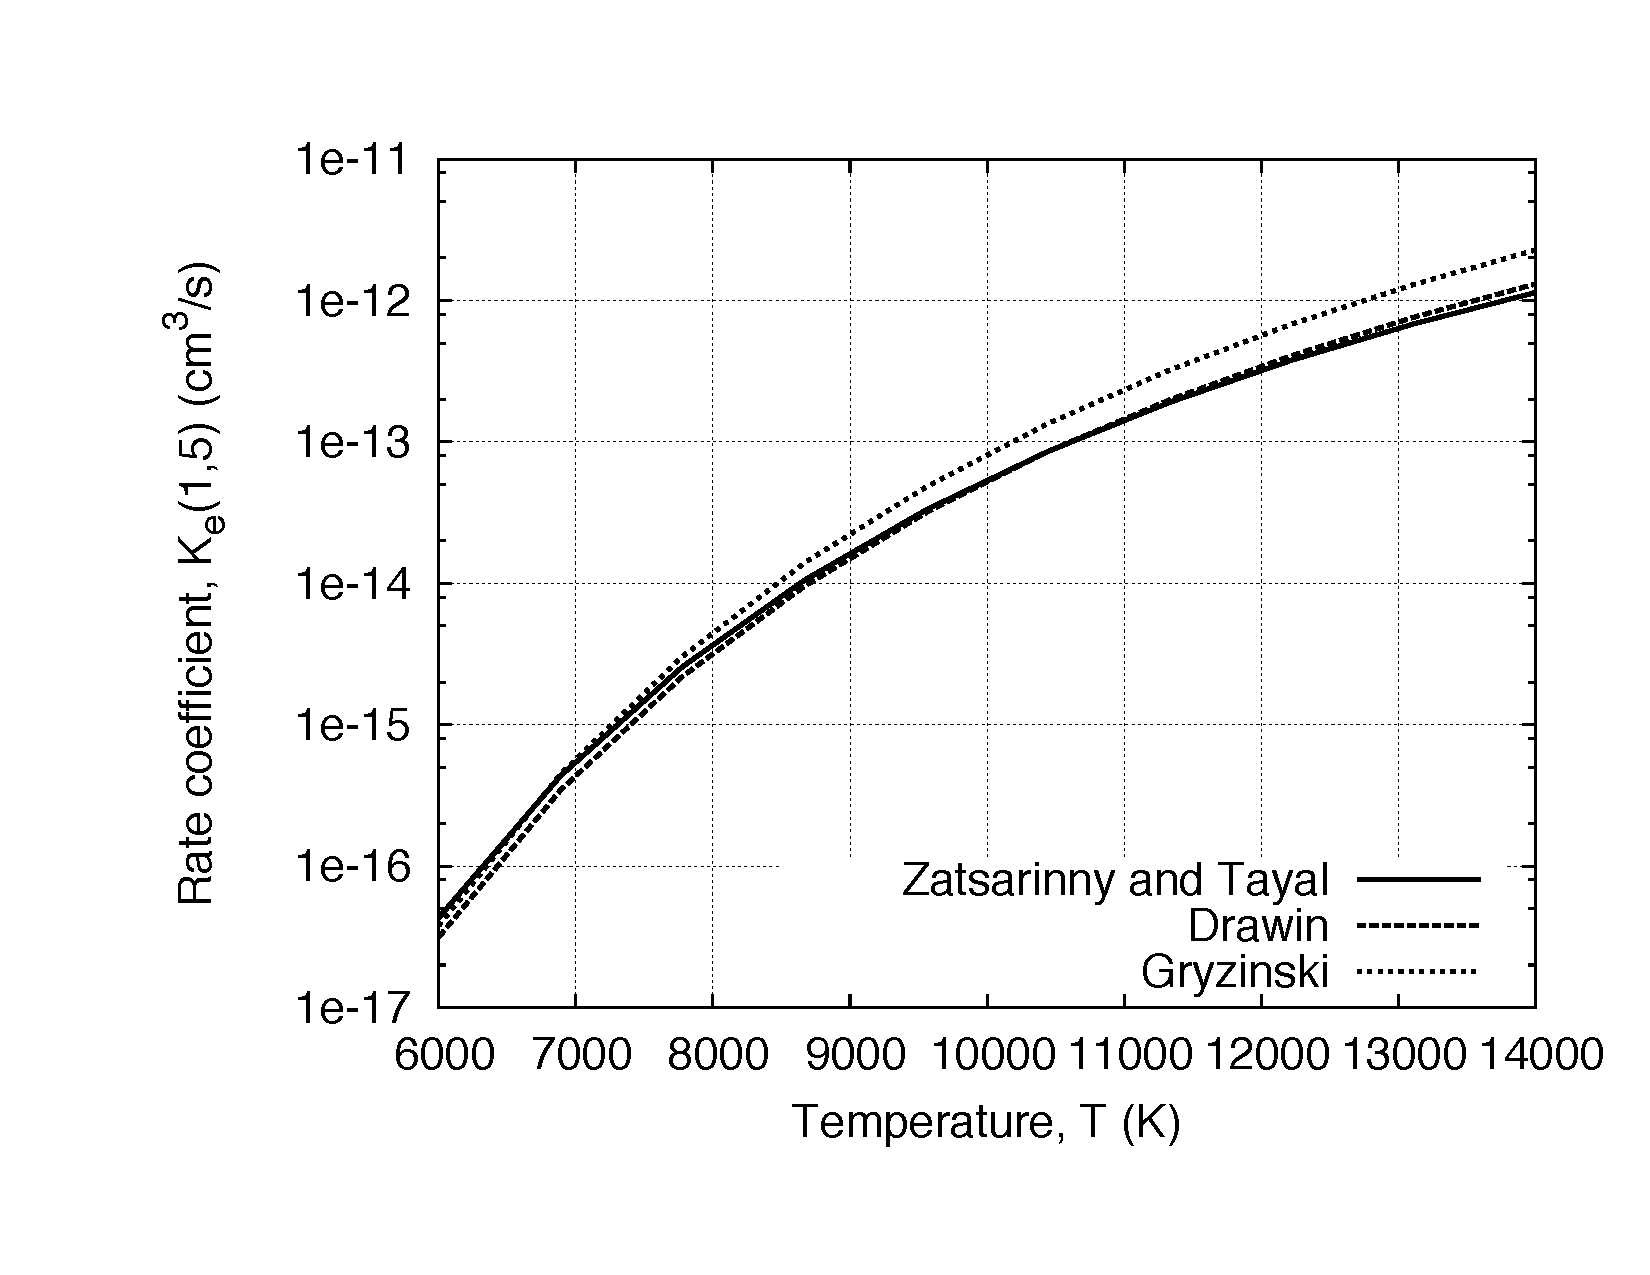
\includegraphics[width=0.48\linewidth]{collisional-radiative-modelling/figures/K_EIE_O_1_to_5.pdf} \label{fig:K_EIE_O_1_to_5}}
 \subfloat[$\Olevtwo \Rightarrow \Olevfive$ (Forbidden)]{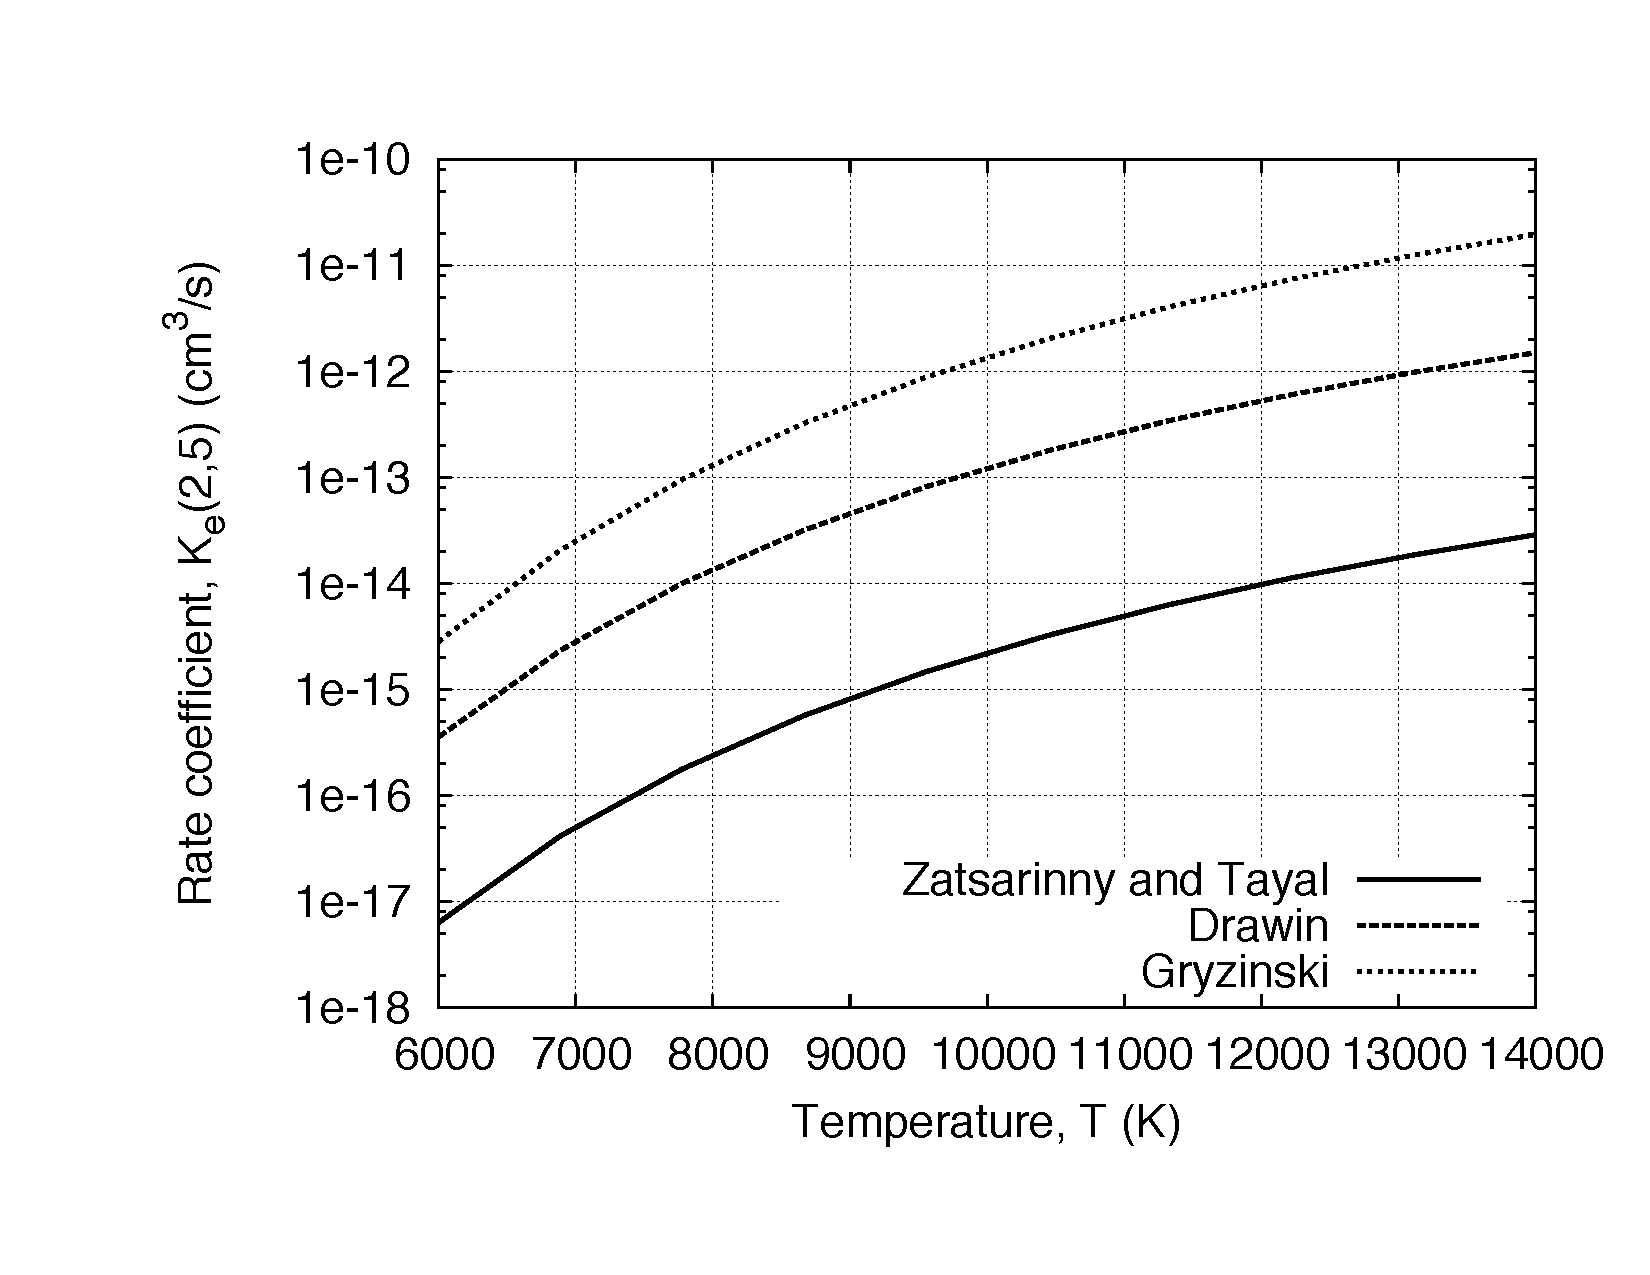
\includegraphics[width=0.48\linewidth]{collisional-radiative-modelling/figures/K_EIE_O_2_to_5.pdf} \label{fig:K_EIE_O_2_to_5}} \\
 \subfloat[$\Olevone \Rightarrow \Olevten$ (Forbidden)]{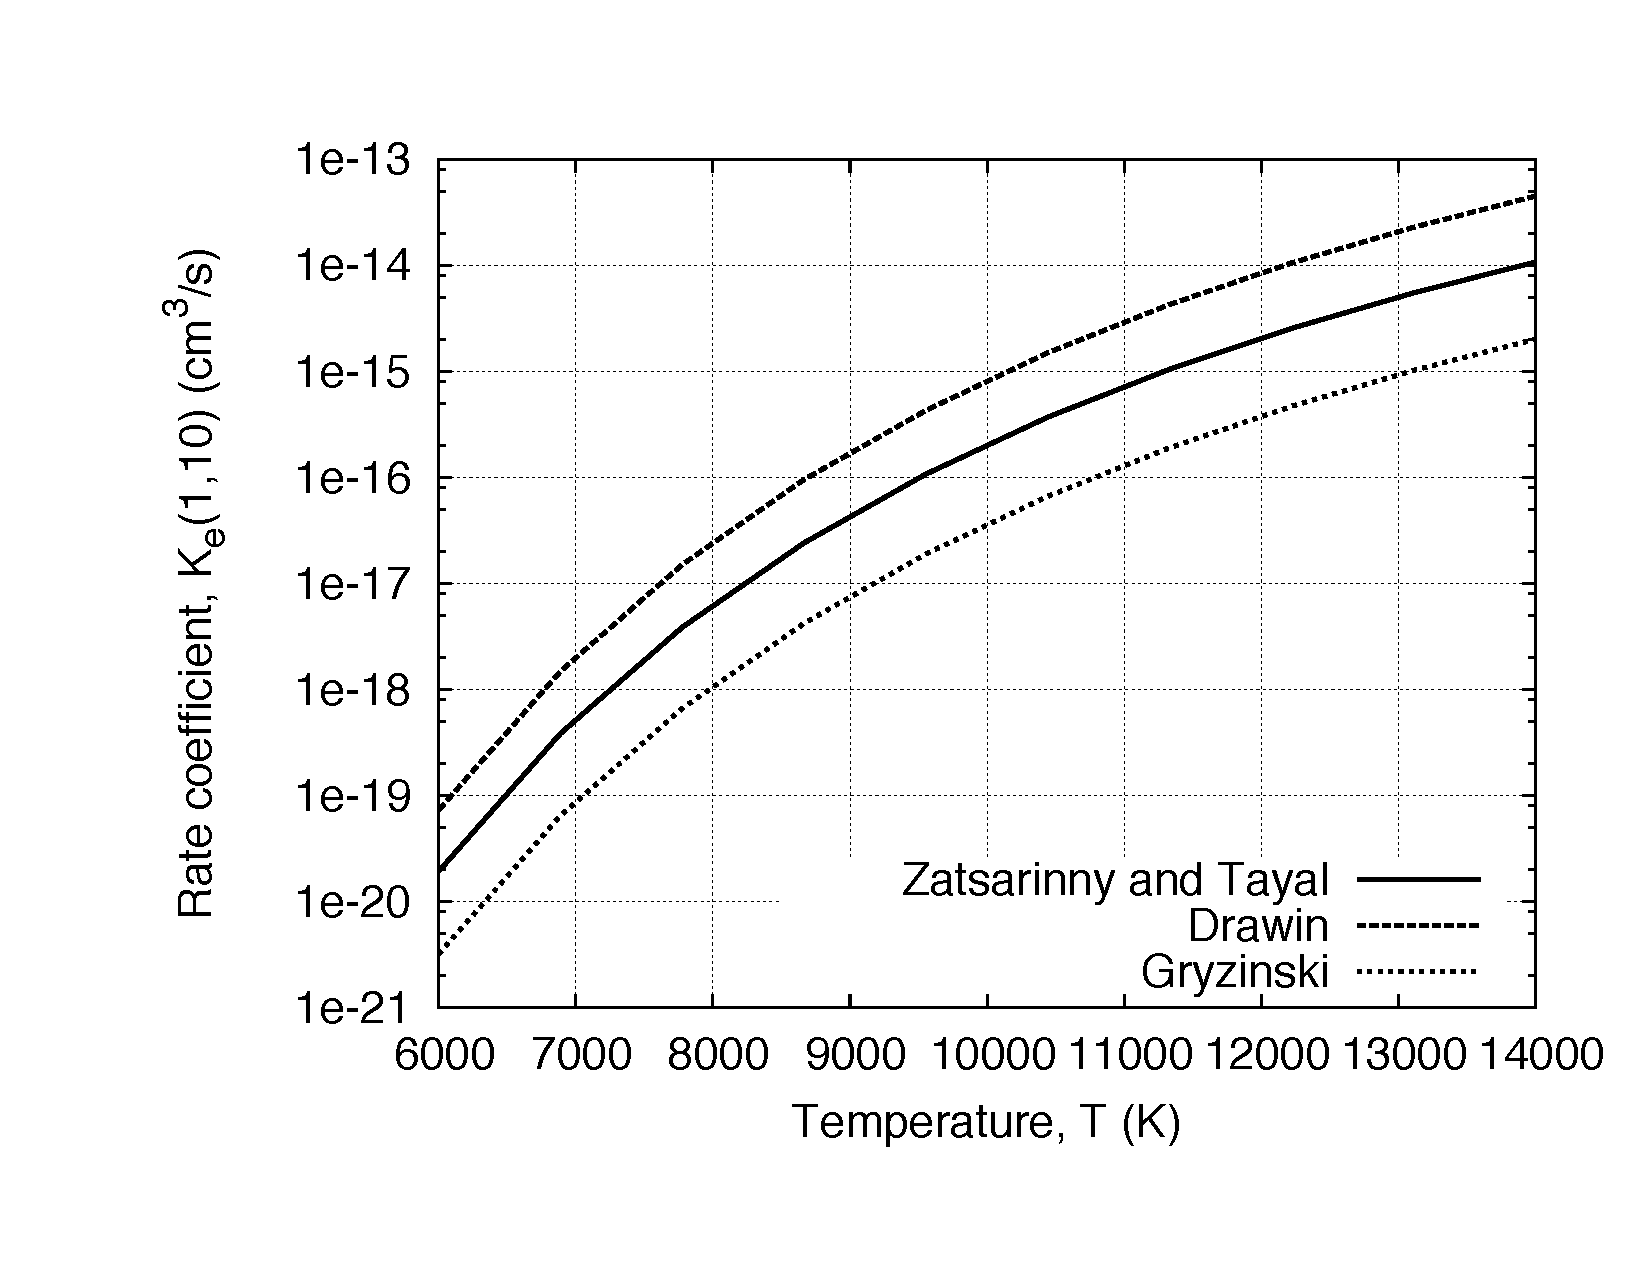
\includegraphics[width=0.48\linewidth]{collisional-radiative-modelling/figures/K_EIE_O_1_to_10.pdf} \label{fig:K_EIE_O_1_to_10}}
 \subfloat[$\Olevthree \Rightarrow \Olevseven$ (Forbidden)]{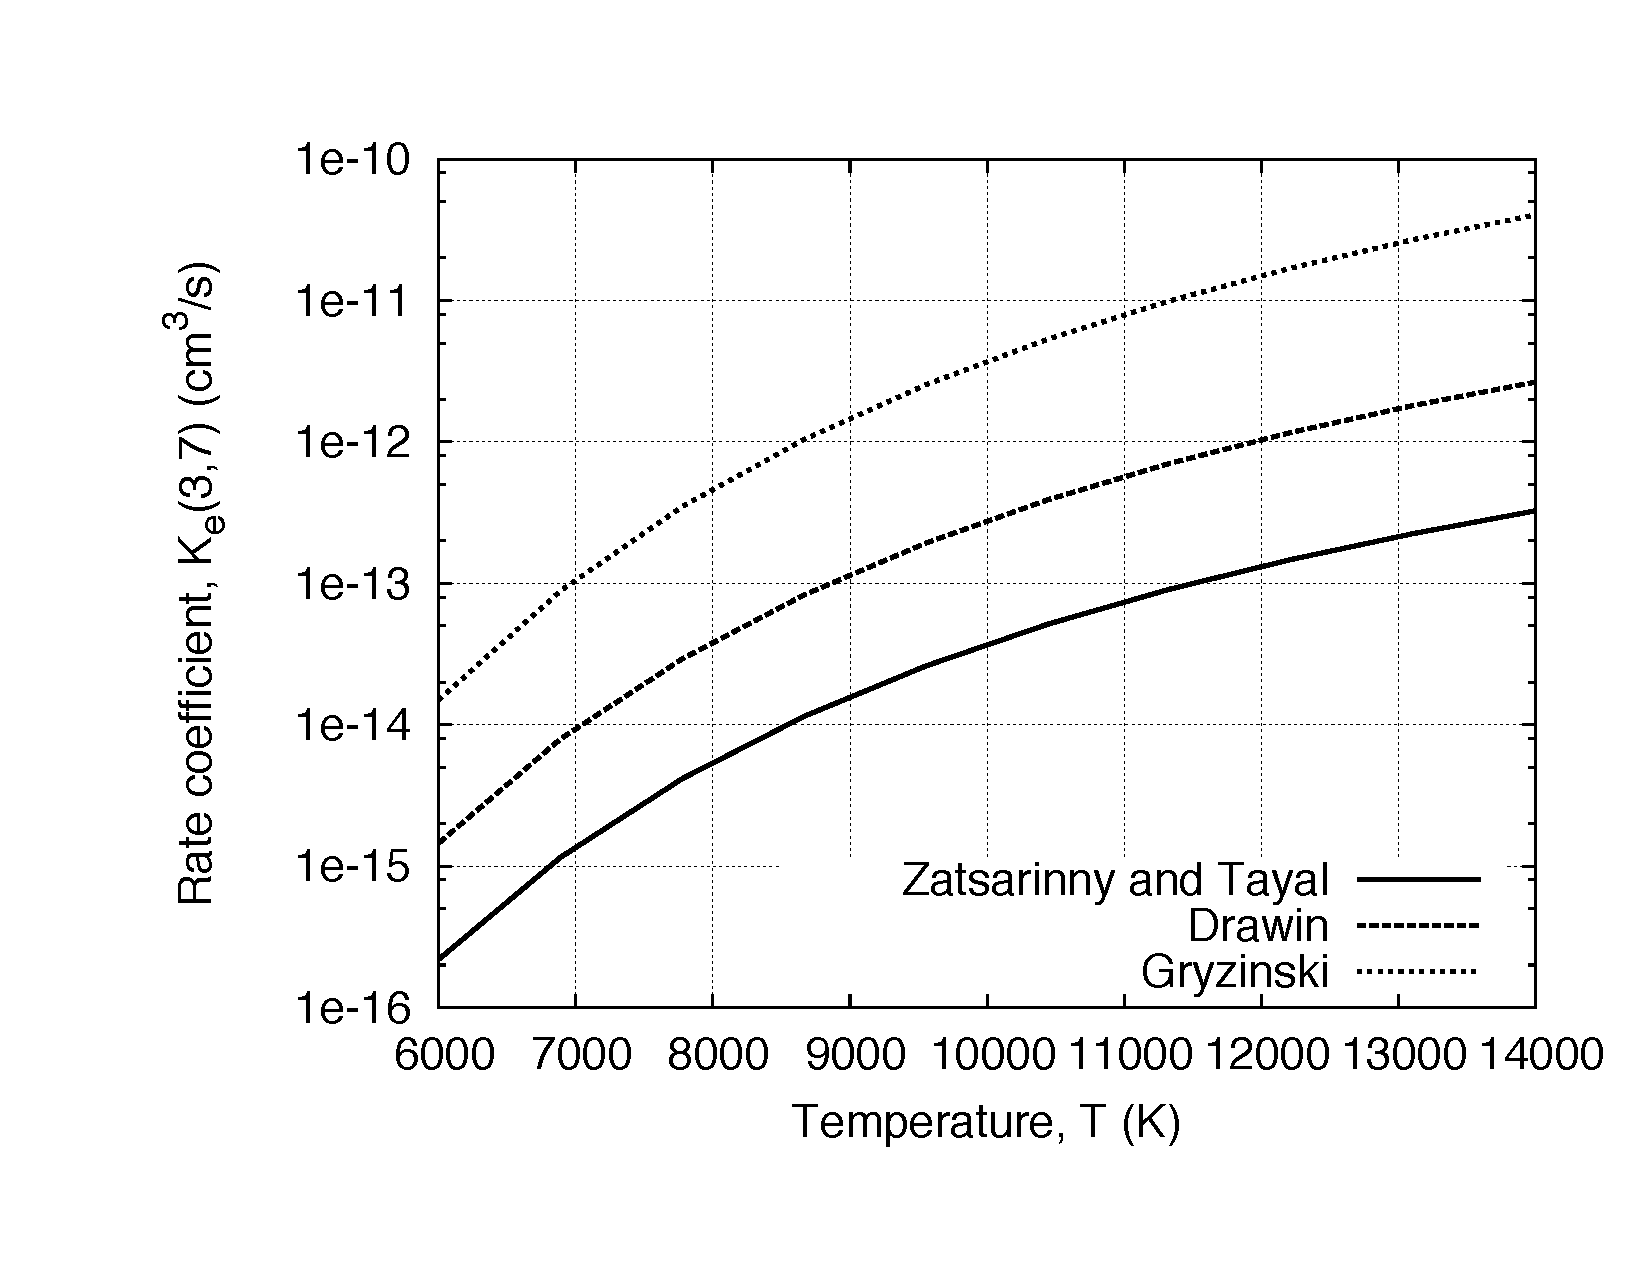
\includegraphics[width=0.48\linewidth]{collisional-radiative-modelling/figures/K_EIE_O_3_to_7.pdf} \label{fig:K_EIE_O_3_to_7}}
 \caption{Comparison of  electron impact excitation rate coefficients for atomic oxygen.}
 \label{fig:K_EIE_O}
\end{figure}
%
\begin{figure}[!hbtp]
 \centering
 \ContinuedFloat
 \subfloat[$\Olevone \Rightarrow \Olevsixteen$ (Allowed)]{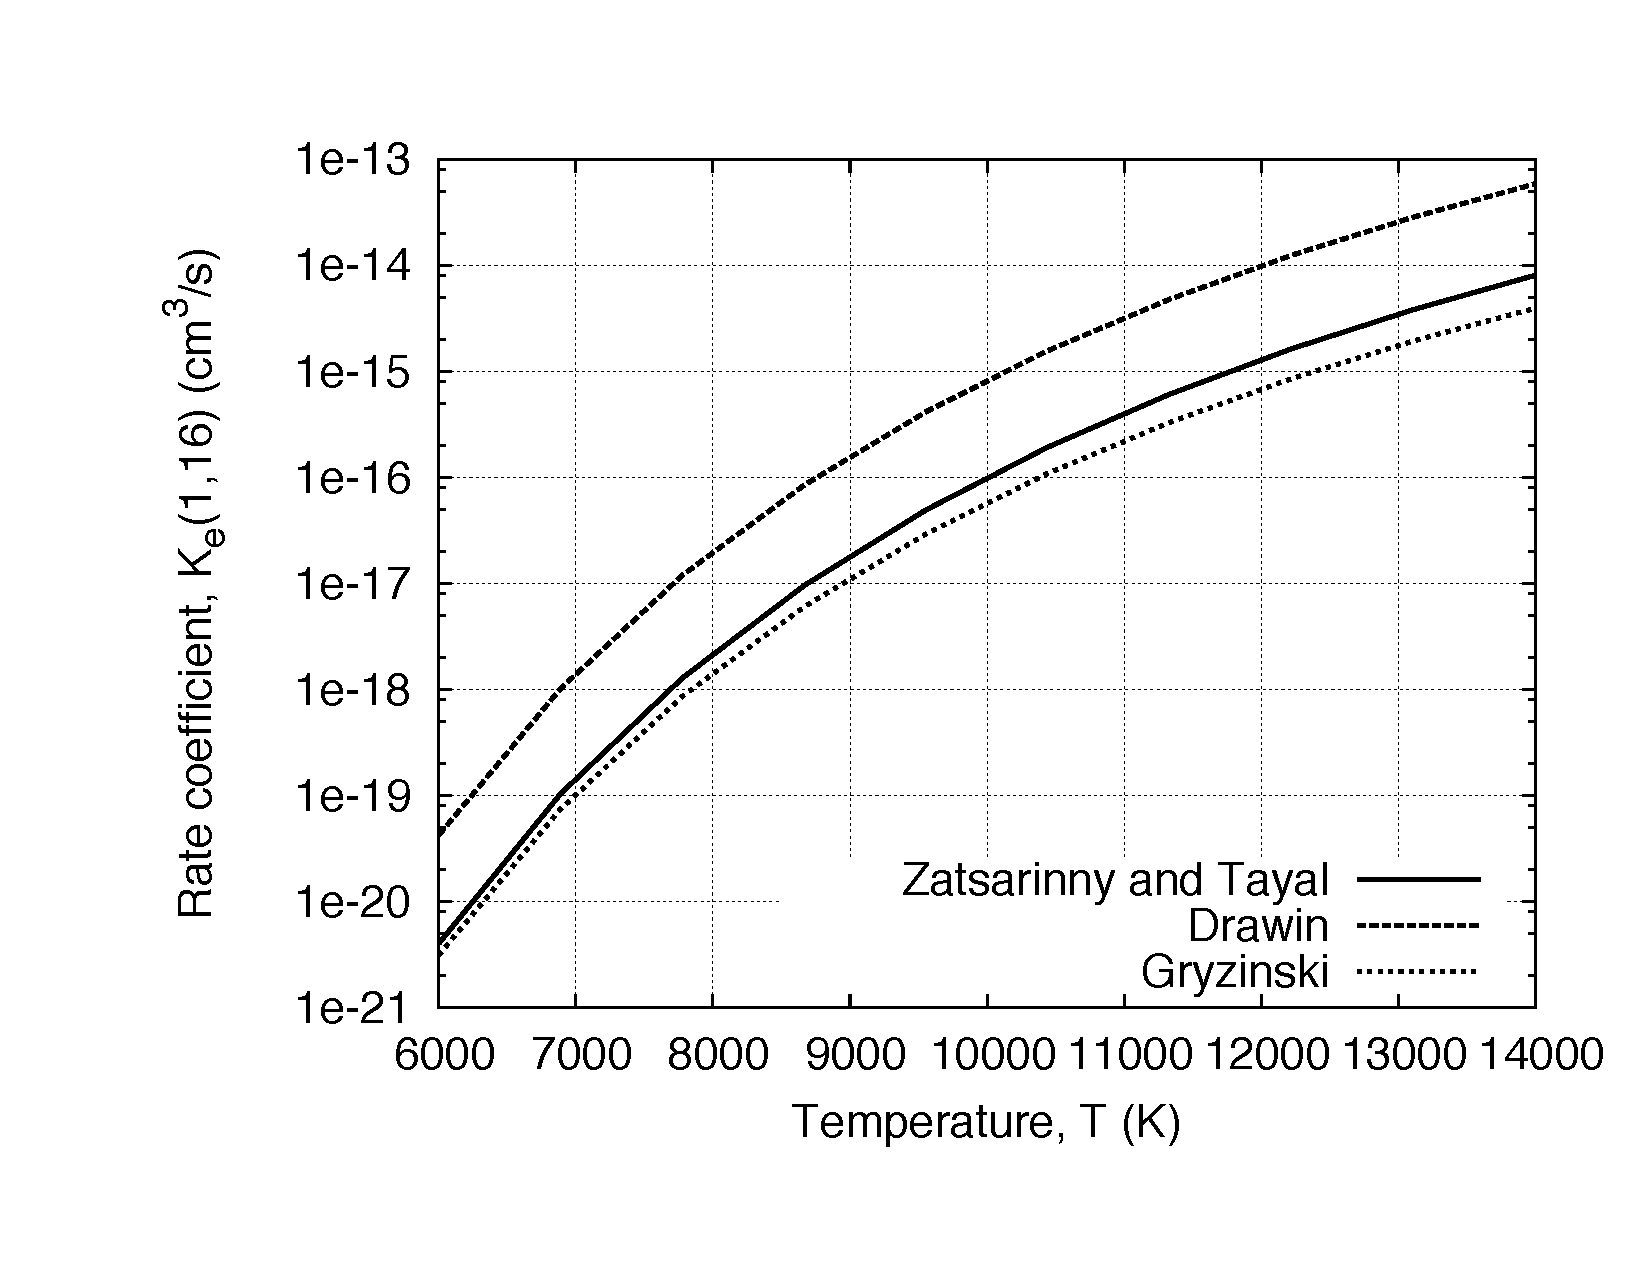
\includegraphics[width=0.48\linewidth]{collisional-radiative-modelling/figures/K_EIE_O_1_to_16.pdf} \label{fig:K_EIE_O_1_to_16}}
 \subfloat[$\Olevone \Rightarrow \Olevseventeen$ (Forbidden)]{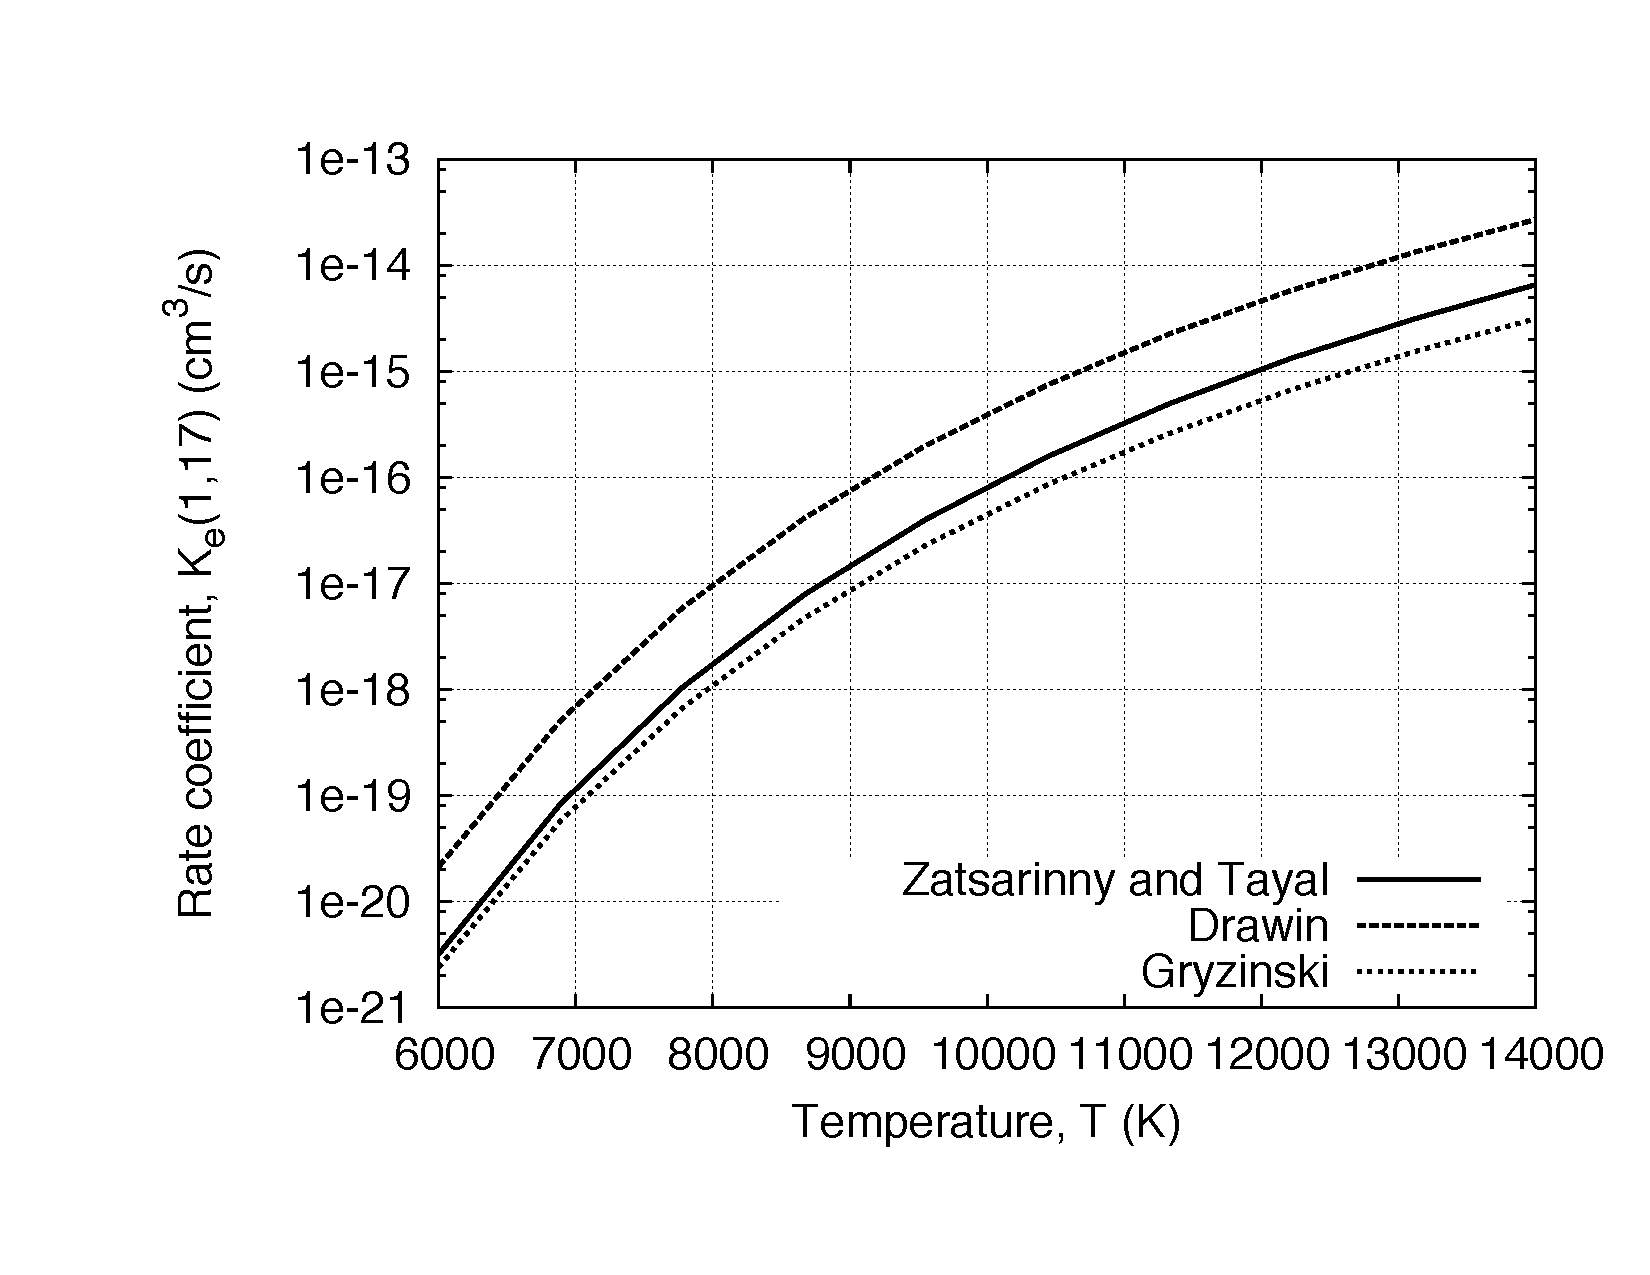
\includegraphics[width=0.48\linewidth]{collisional-radiative-modelling/figures/K_EIE_O_1_to_17.pdf} \label{fig:K_EIE_O_1_to_17}} \\
 \subfloat[$\Olevone \Rightarrow \Olevtwenty$ (Forbidden)]{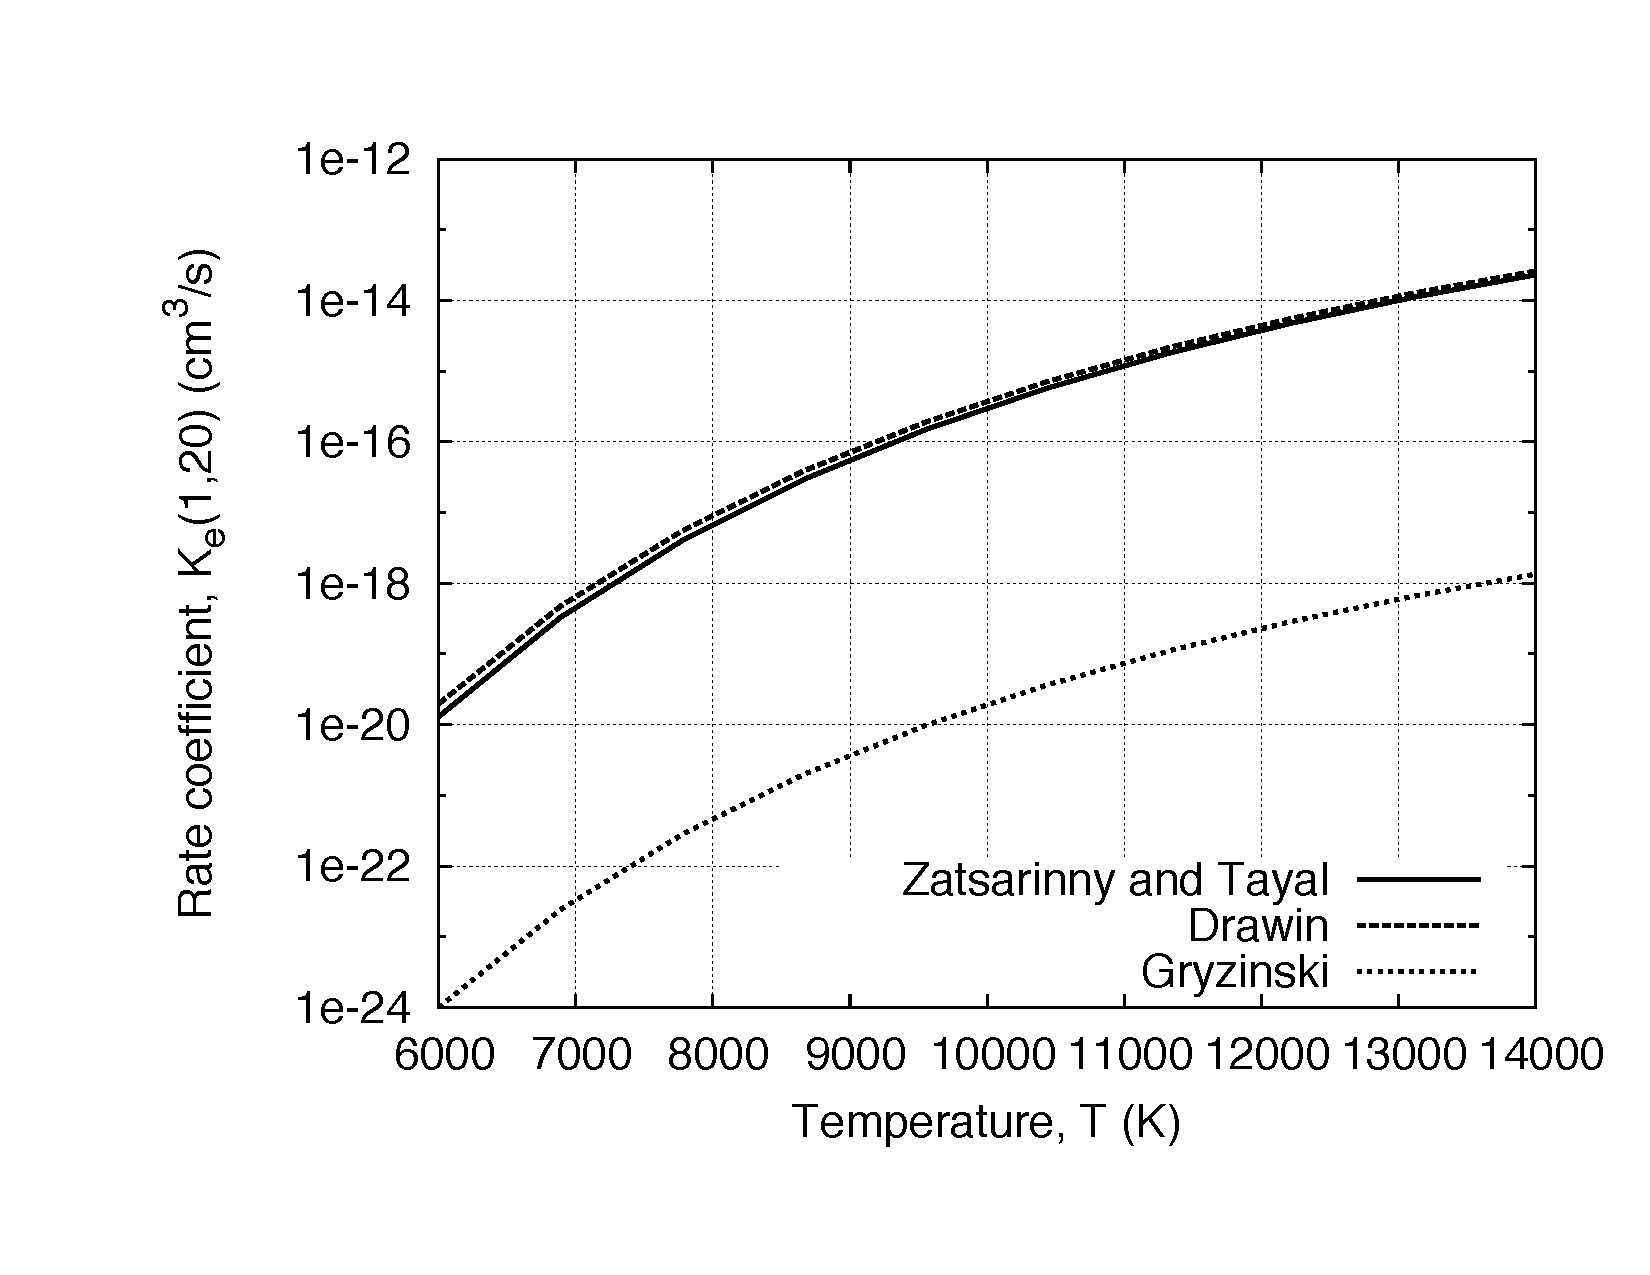
\includegraphics[width=0.48\linewidth]{collisional-radiative-modelling/figures/K_EIE_O_1_to_20.pdf} \label{fig:K_EIE_O_1_to_20}}
 \subfloat[$\Olevtwo \Rightarrow \Olevtwenty$ (Forbidden)]{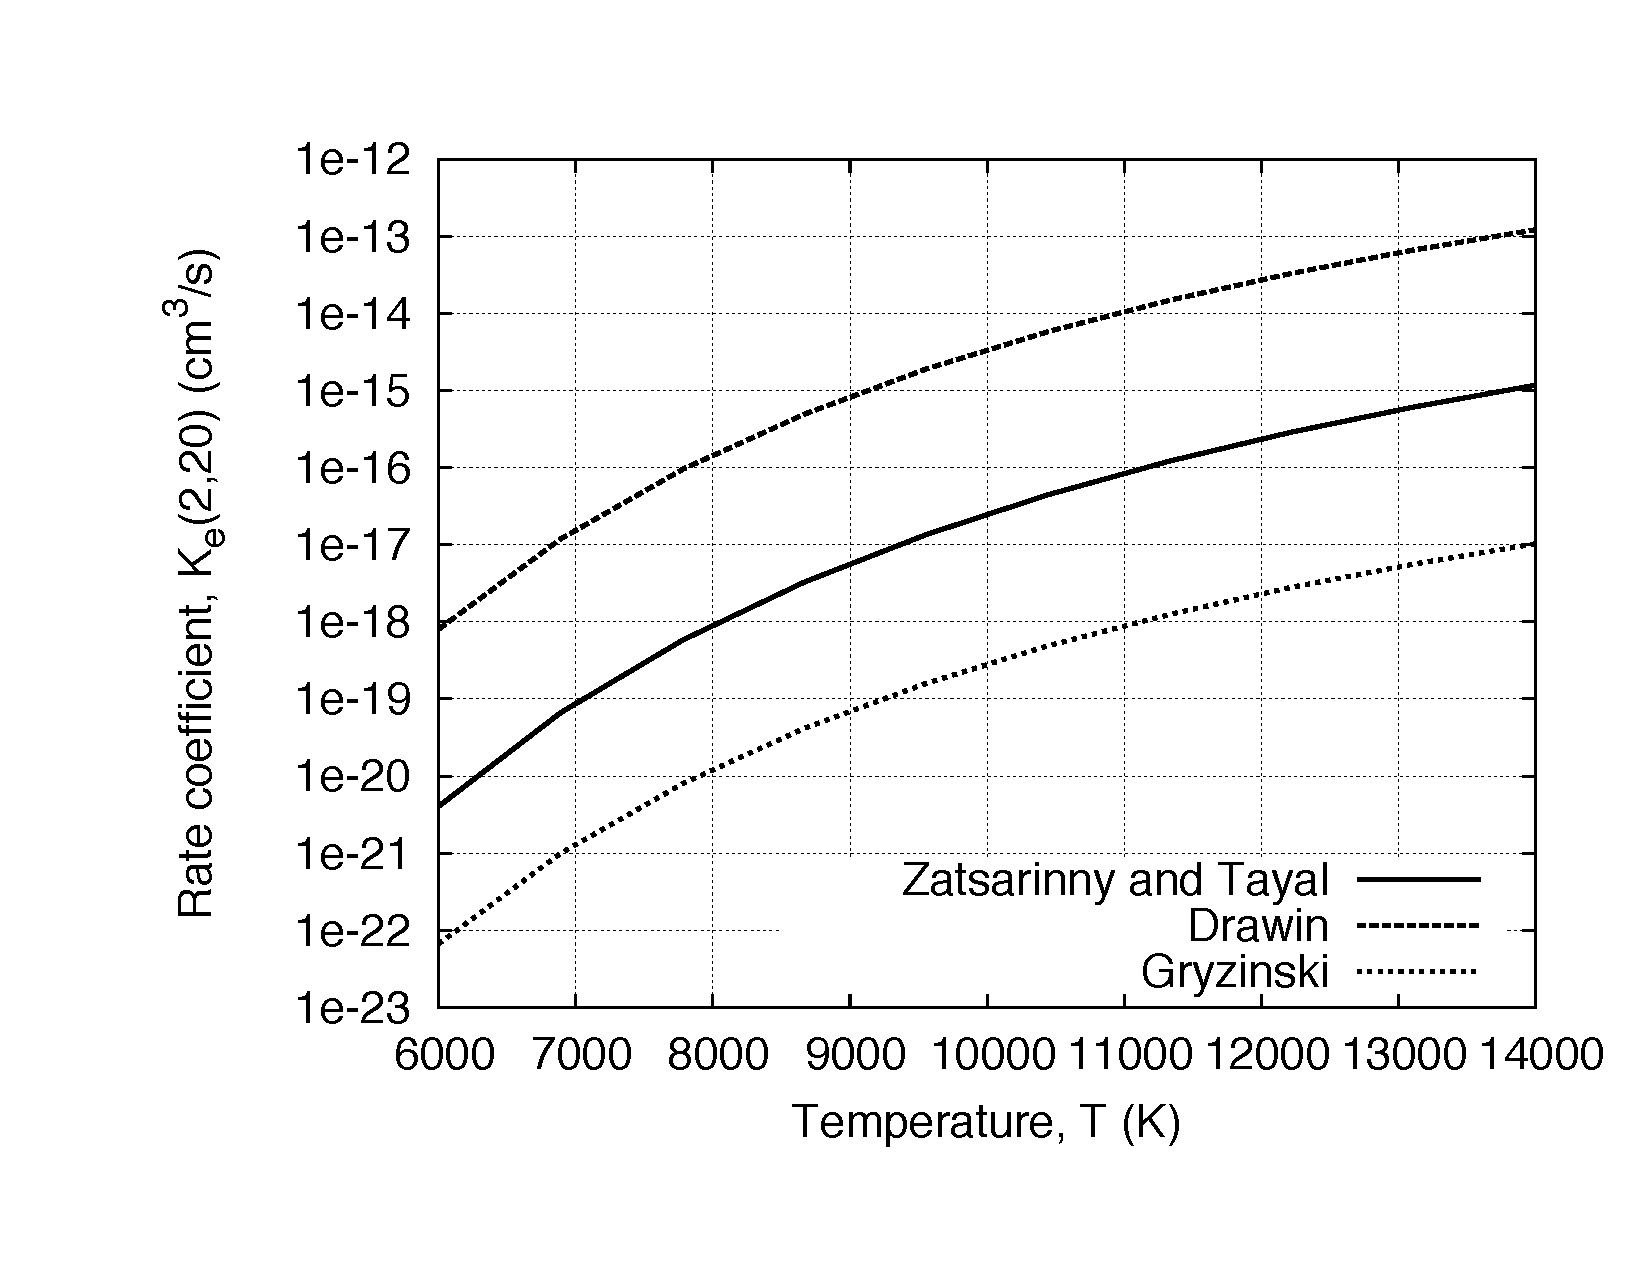
\includegraphics[width=0.48\linewidth]{collisional-radiative-modelling/figures/K_EIE_O_2_to_20.pdf} \label{fig:K_EIE_O_2_to_20}} \\
 \caption{\textit{(Continued)} Comparison of  electron impact excitation rate coefficients for atomic oxygen.}
 \label{fig:K_EIE_O}
\end{figure}

\subsubsection{Electron impact ionisation of O}

Johnston~\cite{JohnPhd} implemented the ionisation rate coefficients proposed by Soon and Kunc~\cite{SK1990} for the ground and first two excited levels of atomic oxygen.
The rate coefficients are calculated as described in Equations~\ref{eq:K_EII_Soon_Kunc_a} to~\ref{eq:K_EII_Soon_Kunc_c}, where $A=30.52$ and $\chi=4.0$ for levels $i$=1, 2 and 3 of O.
This expression is a curve-fit based on the rate coefficient derived from experimentally measured electron impact ionisation cross sections for the ground state of O.

\par

Panesi~\cite{panesi_phd} implemented the ionisation rate coefficients presented by Bultel \textit{et al.}~\cite{BBB+2006}, which were obtained from the compilation of Tawara and Kato~\cite{TK1999} and the combined binary-encounter Bethe (BEB) and scaled plane-wave Born (PWB) calculations of Kim and Desclaux~\cite{KD2002}.
The rates for the ground and first two excited states of O were presented as generalised Arrhenius curve-fits in the temperature range 2,000 $\leq T_e \leq$ 10,000\,K.

\par

Figure~\ref{fig:K_EII_O} compares the electron impact ionisation rate coefficient for various transitions of O.
Again, the Bultel rates are anomalous and are not thought to be accurate for the temperature range of present interest.
The two Drawin models bound the experimentally fitted model of Kunc and Soon~\cite{KS1989}, with Panesi's implementation being in closer agreement, especially for ionisation of the $\Olevthree$ multiplet (see Figure~\ref{fig:K_EII_O_3}).
Similarly as for atomic nitrogen, Johnston's implementation of the Drawin cross sections is between approximately 2 and 100 times smaller than Panesi's implementation for all levels.
Therefore in the present work the electron impact ionisation coefficients of Kunc and Soon~\cite{KS1989} are preferred for the first three levels, while the Drawin model implemented by Panesi~\cite{JohnPhd} is used for the remaining levels.

\begin{figure}[h]
 \centering
 \subfloat[$\text{O } \Olevone \Rightarrow \text{O}^+$]{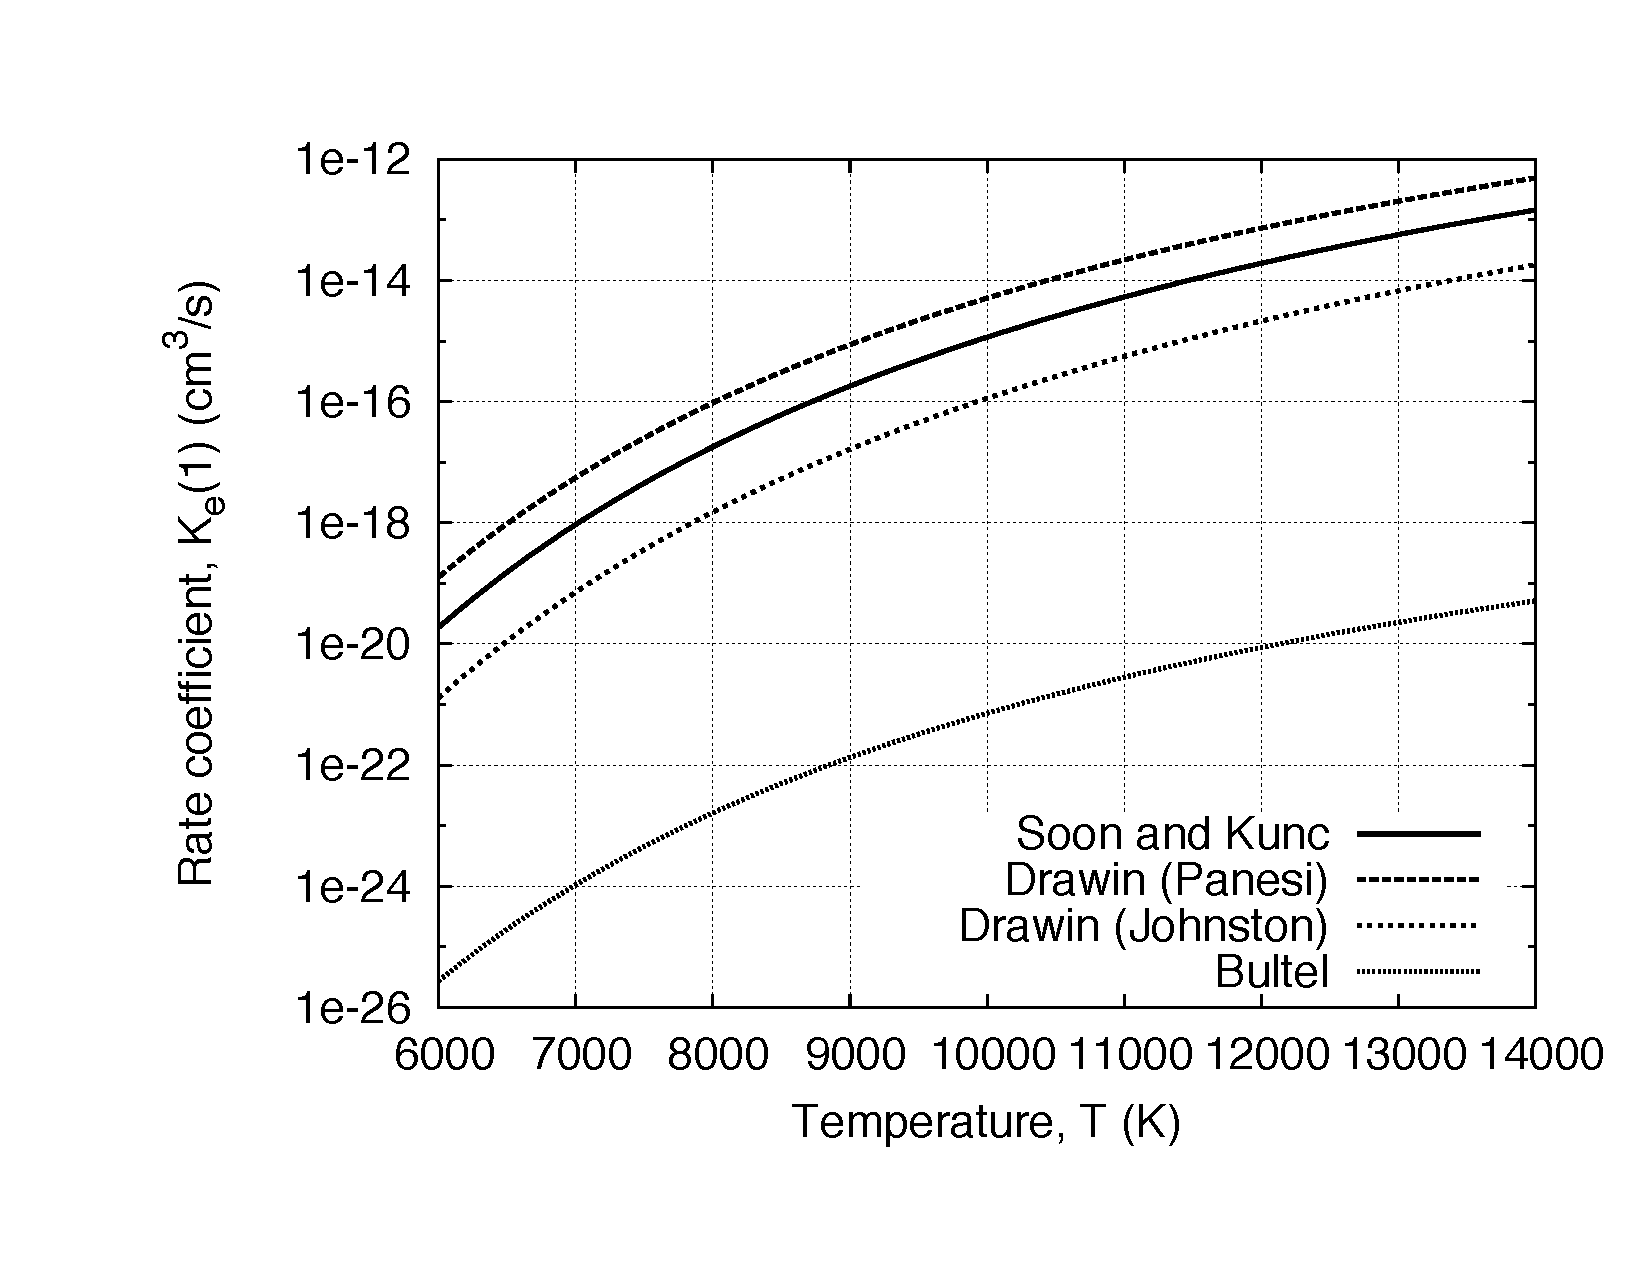
\includegraphics[width=0.48\linewidth]{collisional-radiative-modelling/figures/K_EII_O_1.pdf} \label{fig:K_EII_O_1}}
 \subfloat[$\text{O } \Olevtwo \Rightarrow \text{O}^+$]{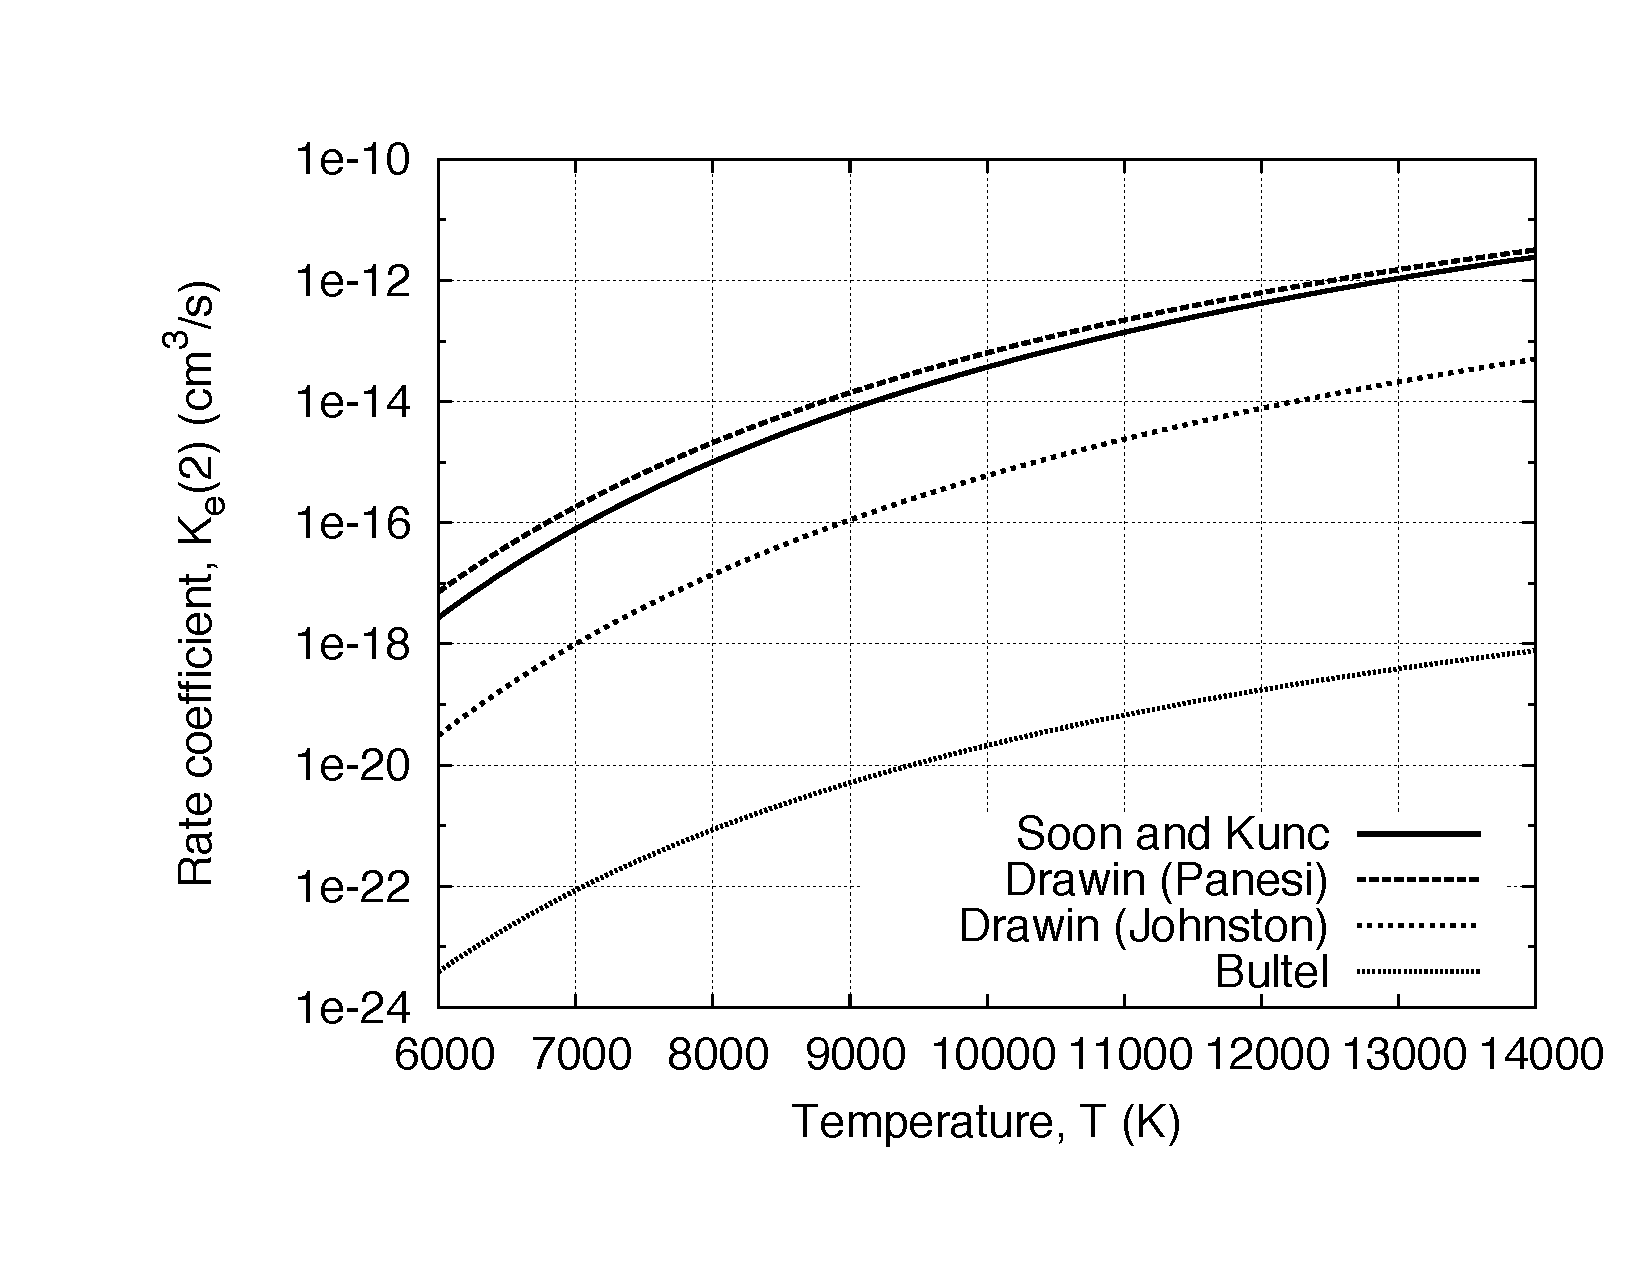
\includegraphics[width=0.48\linewidth]{collisional-radiative-modelling/figures/K_EII_O_2.pdf} \label{fig:K_EII_O_2}} \\
 \subfloat[$\text{O } \Olevthree \Rightarrow \text{O}^+$]{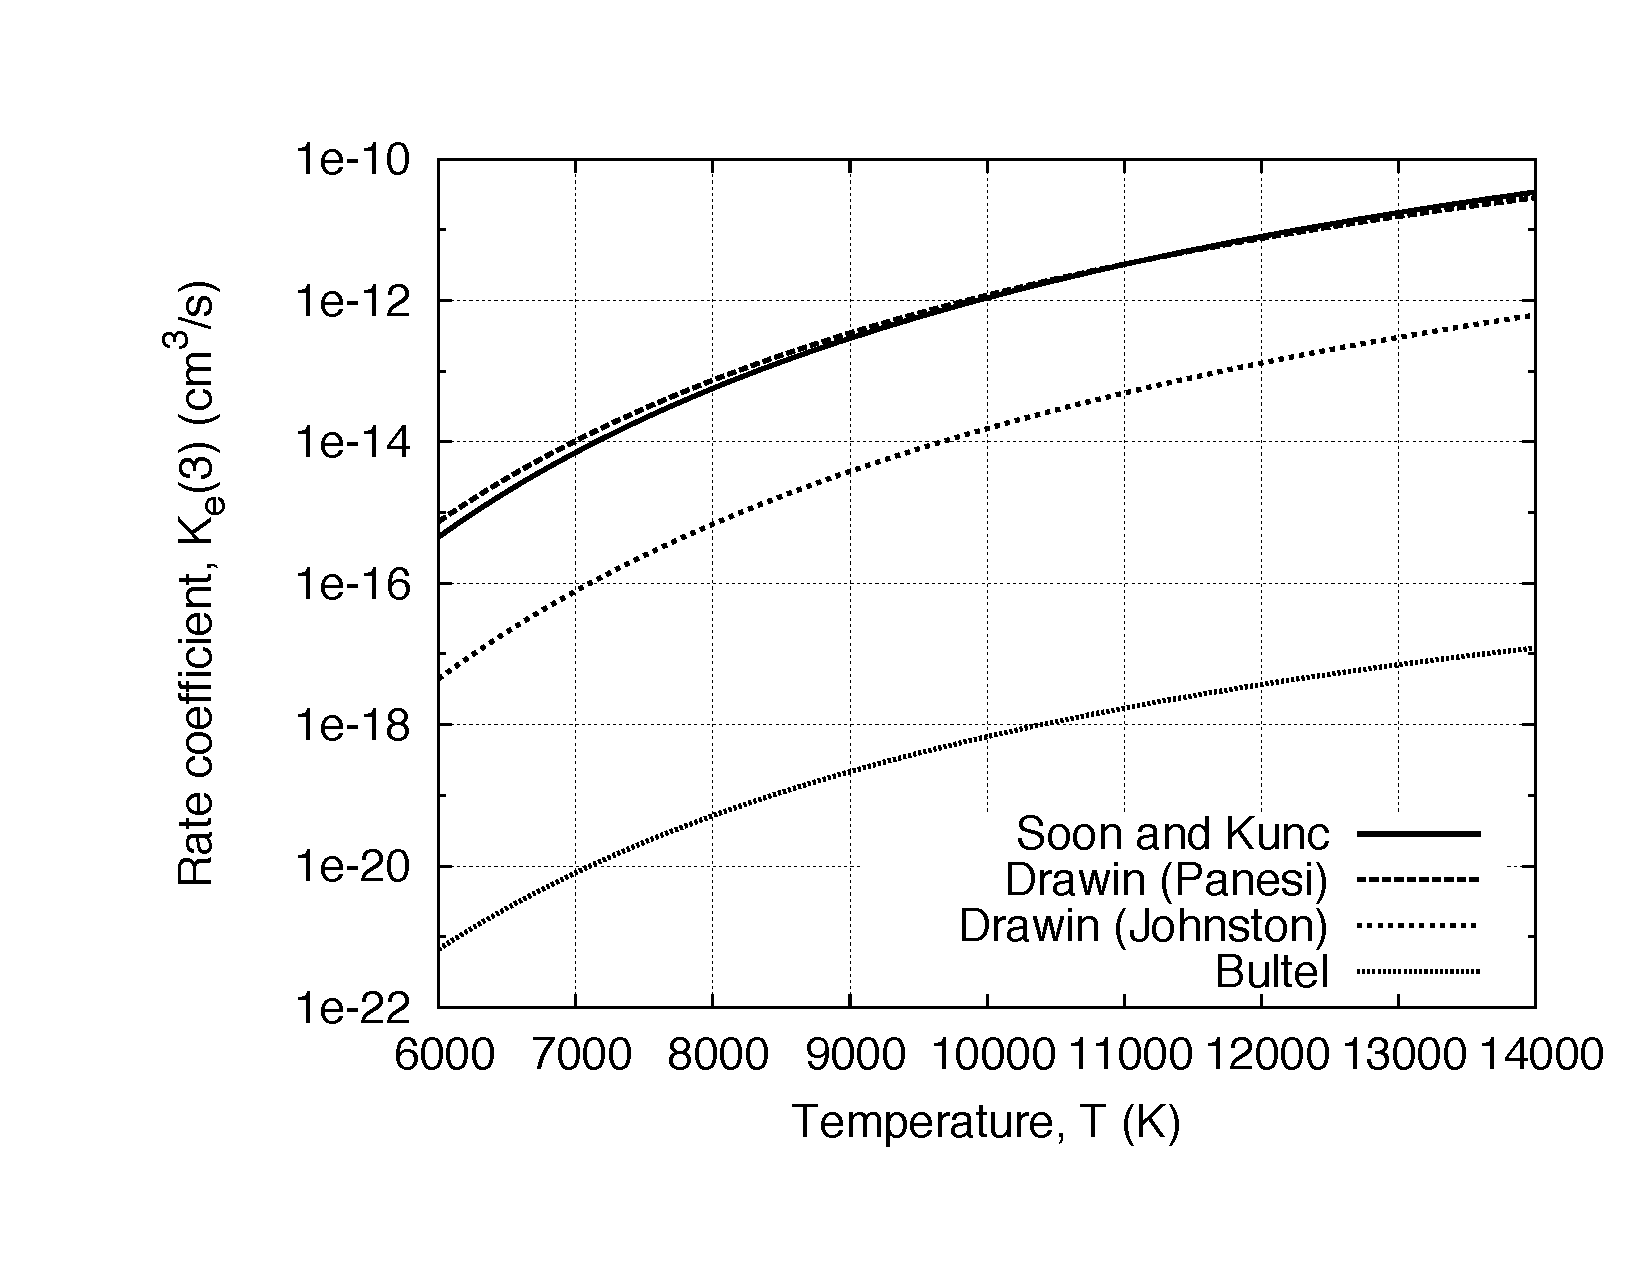
\includegraphics[width=0.48\linewidth]{collisional-radiative-modelling/figures/K_EII_O_3.pdf} \label{fig:K_EII_O_3}}
 \subfloat[$\text{O } \Olevsixteen \Rightarrow \text{O}^+$]{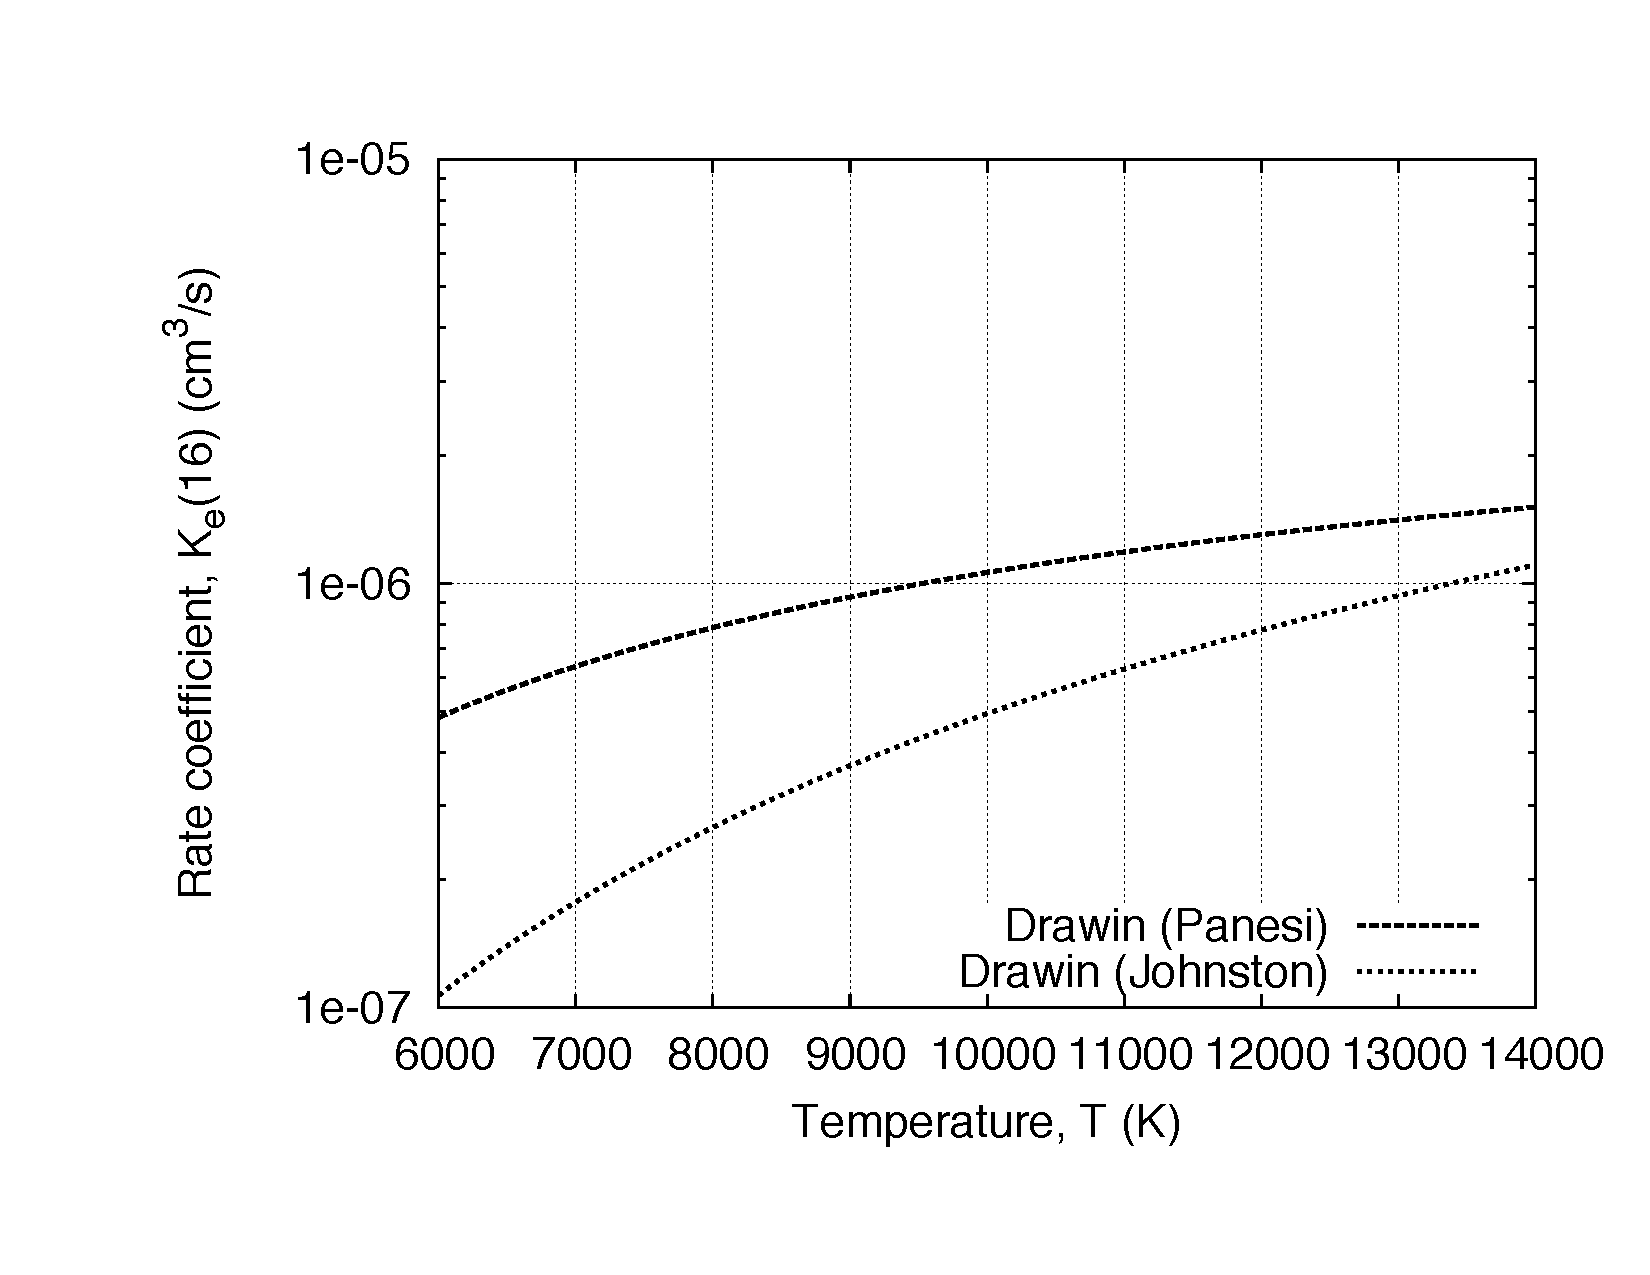
\includegraphics[width=0.48\linewidth]{collisional-radiative-modelling/figures/K_EII_O_16.pdf} \label{fig:K_EII_O_13}}
 \caption{Comparison of  electron impact ionisation rate coefficients for atomic oxygen.}
 \label{fig:K_EII_O}
\end{figure}

\subsubsection{(b) Diatomic species: N$_2$ and N$_2+$}

Johnston~\cite{JohnPhd} presented collisional-radiative models for N$_2$ and N$_2^+$ compiled from both theoretically calculated and experimentally measured rate-coefficients in the literature.
The majority of the collisional rate coefficients are based on the theoretical calculations of Teulet \textit{et al.}~\cite{TSG1999}, however other more accurate data was preferenced where available.
Since Johnston formulated this model, a set of collisional rate coefficients for the diatomic species CN, CO, N$_2$, N$_2^+$, O$_2$ and NO have been proposed by Park~\cite{park2008a, park2008b}.
The rate coefficients are based on experimentally measured cross sections where available, and theoretically estimated otherwise.

\par

\begin{figure}[t]
 \centering
 \subfloat[$\NNlevX \Longrightarrow \NNlevB$]{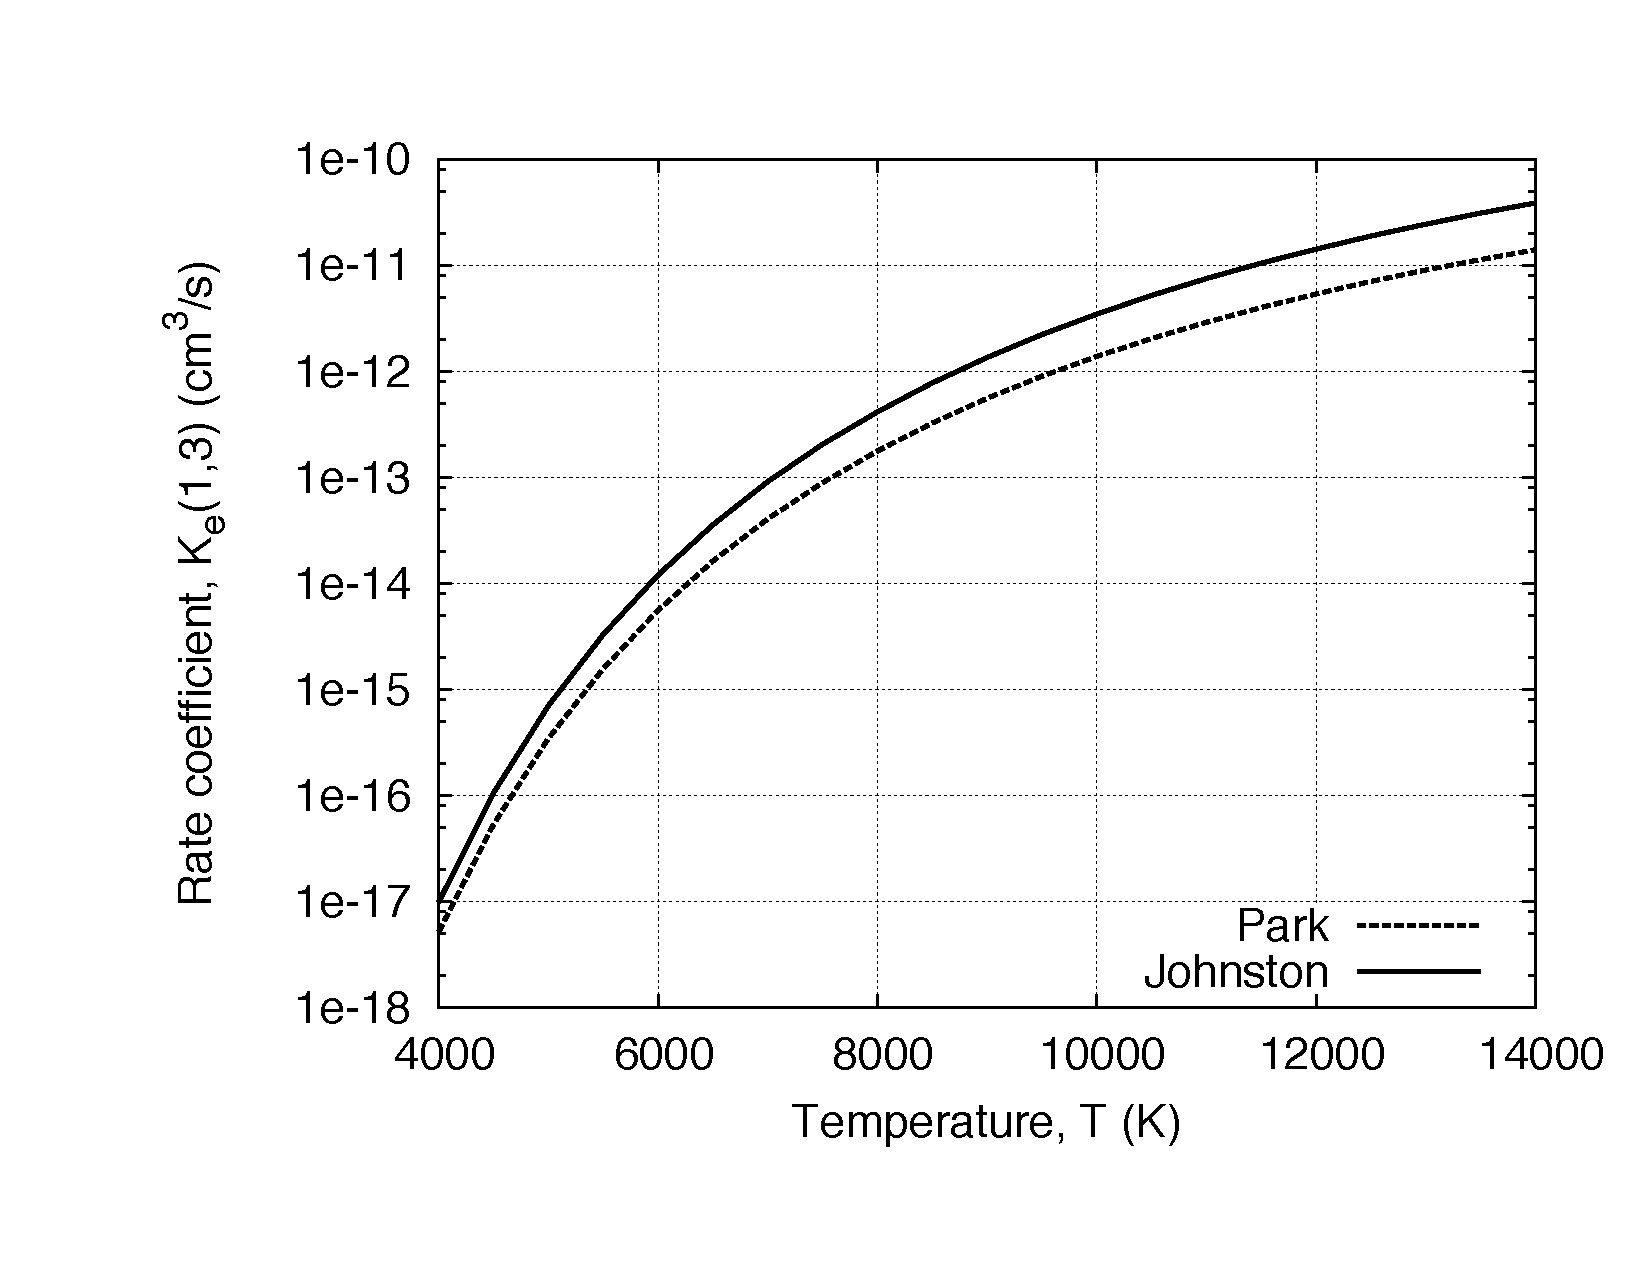
\includegraphics[width=0.48\linewidth]{collisional-radiative-modelling/figures/K_EIE_N2_X_to_B.pdf} \label{fig:K_EIE_N2_X_to_B}}
 \subfloat[$\NNlevA \Longrightarrow \NNlevB$]{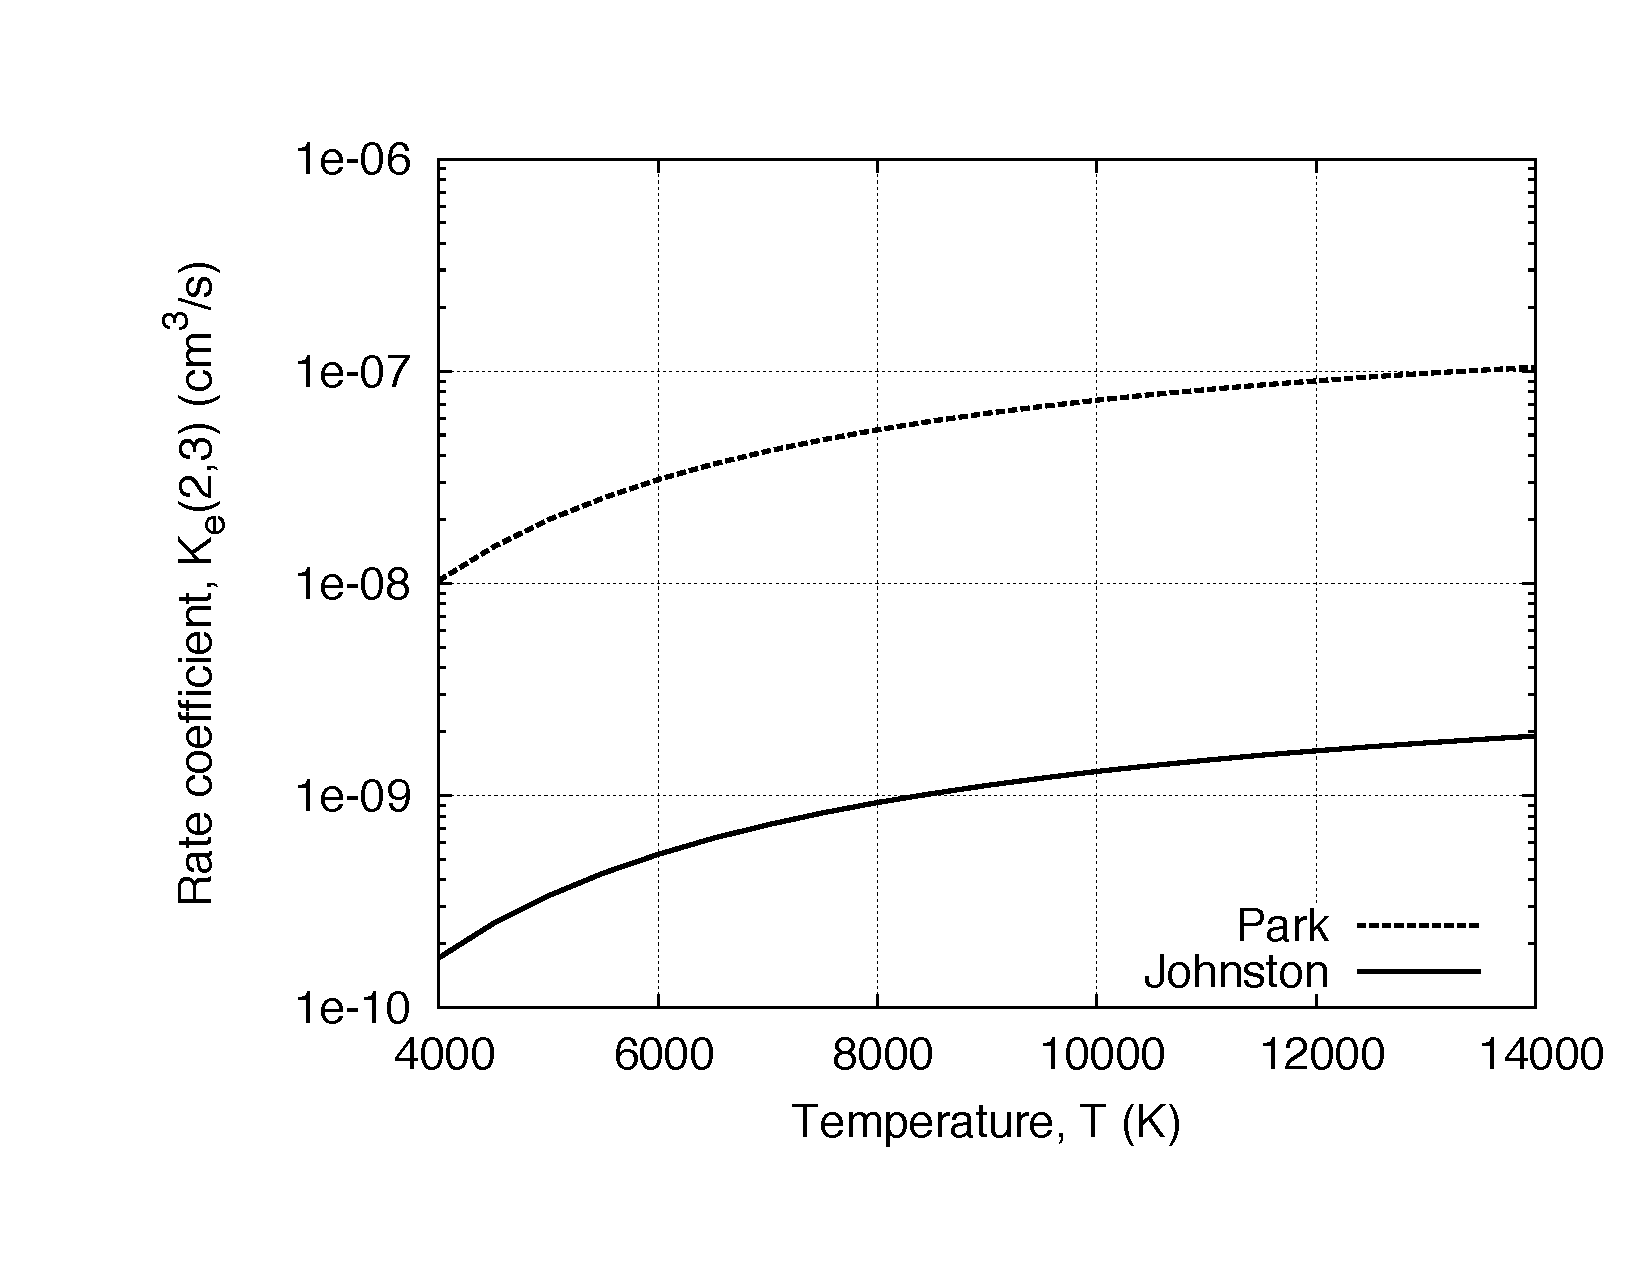
\includegraphics[width=0.48\linewidth]{collisional-radiative-modelling/figures/K_EIE_N2_A_to_B.pdf} \label{fig:K_EIE_N2_A_to_B}}
 \caption{Comparison of electron impact excitation rate coefficients for transitions to the $\NNlevB$ state of N$_2$.}
 \label{fig:K_EIE_N2}
\end{figure}

The most critical reactions for N$_2$ and N$_2^+$ at Earth re-entry conditions are those populating the upper states of radiative transitions via electron impact excitation.
Figure~\ref{fig:K_EIE_N2} compares the electron impact excitation rates populating the $\NNlevB$ state of N$_2$ (upper state for the First Positive band system), and Figure~\ref{fig:K_EIE_N2_plus} compares the electron impact excitation rates populating the $\NNplevB$ state of N$_2^+$ (upper state for the First Negative band system).
While the two models agree to within a factor of 4 for the \PIEreac{N$_2$}{e$^-$}{\NNlevX}{\NNlevB} transition, Figure~\ref{fig:K_EIE_N2_X_to_B}, the Park rates are substantially higher than those of Johnston for the other transitions.
For the \PIEreac{N$_2$}{e$^-$}{\NNplevA}{\NNplevB} transition in Figure~\ref{fig:K_EIE_N2_plus_A_to_B}, for example, the Park rate is almost four orders of magnitude greater than the Johnston rate.
Although not shown here, the estimated rate of Teulet \textit{et al.}~\cite{TSG1999} for the \PIEreac{N$_2^+$}{e$^-$}{\NNplevX}{\NNplevB} transition is quite similar to the Park rate.
In Johnston's~\cite{JohnPhd} survey of the literature, this rate of Teulet was found to overestimate those from more accurate theoretical calculations.
Furthermore, in Reference~\cite{CJ_EAST_2008} the rates of Teulet were required to be reduced by factors of 10 and 70 for N$_2$ and N$_2^+$ respectively in order to achieve agreement with experiment.
In the present work therefore we choose to adopt the Johnston~\cite{JohnPhd} model.
The collisional-radiative models for N$_2$ and N$_2^+$ are summarised in \textsection~\ref{sec:N2_CR} and~\ref{sec:N2p_CR} respectively.
The nonequilibrium levels considered for N$_2$ are $\NNlevX$, $\NNlevA$, $\NNlevB$ and $\NNlevC$, while those for N$_2^+$ are $\NNplevX$, $\NNplevA$, $\NNplevB$ and $\NNplevC$.

\begin{figure}[h!]
 \centering
 \subfloat[$\NNplevX \Longrightarrow \NNplevB$]{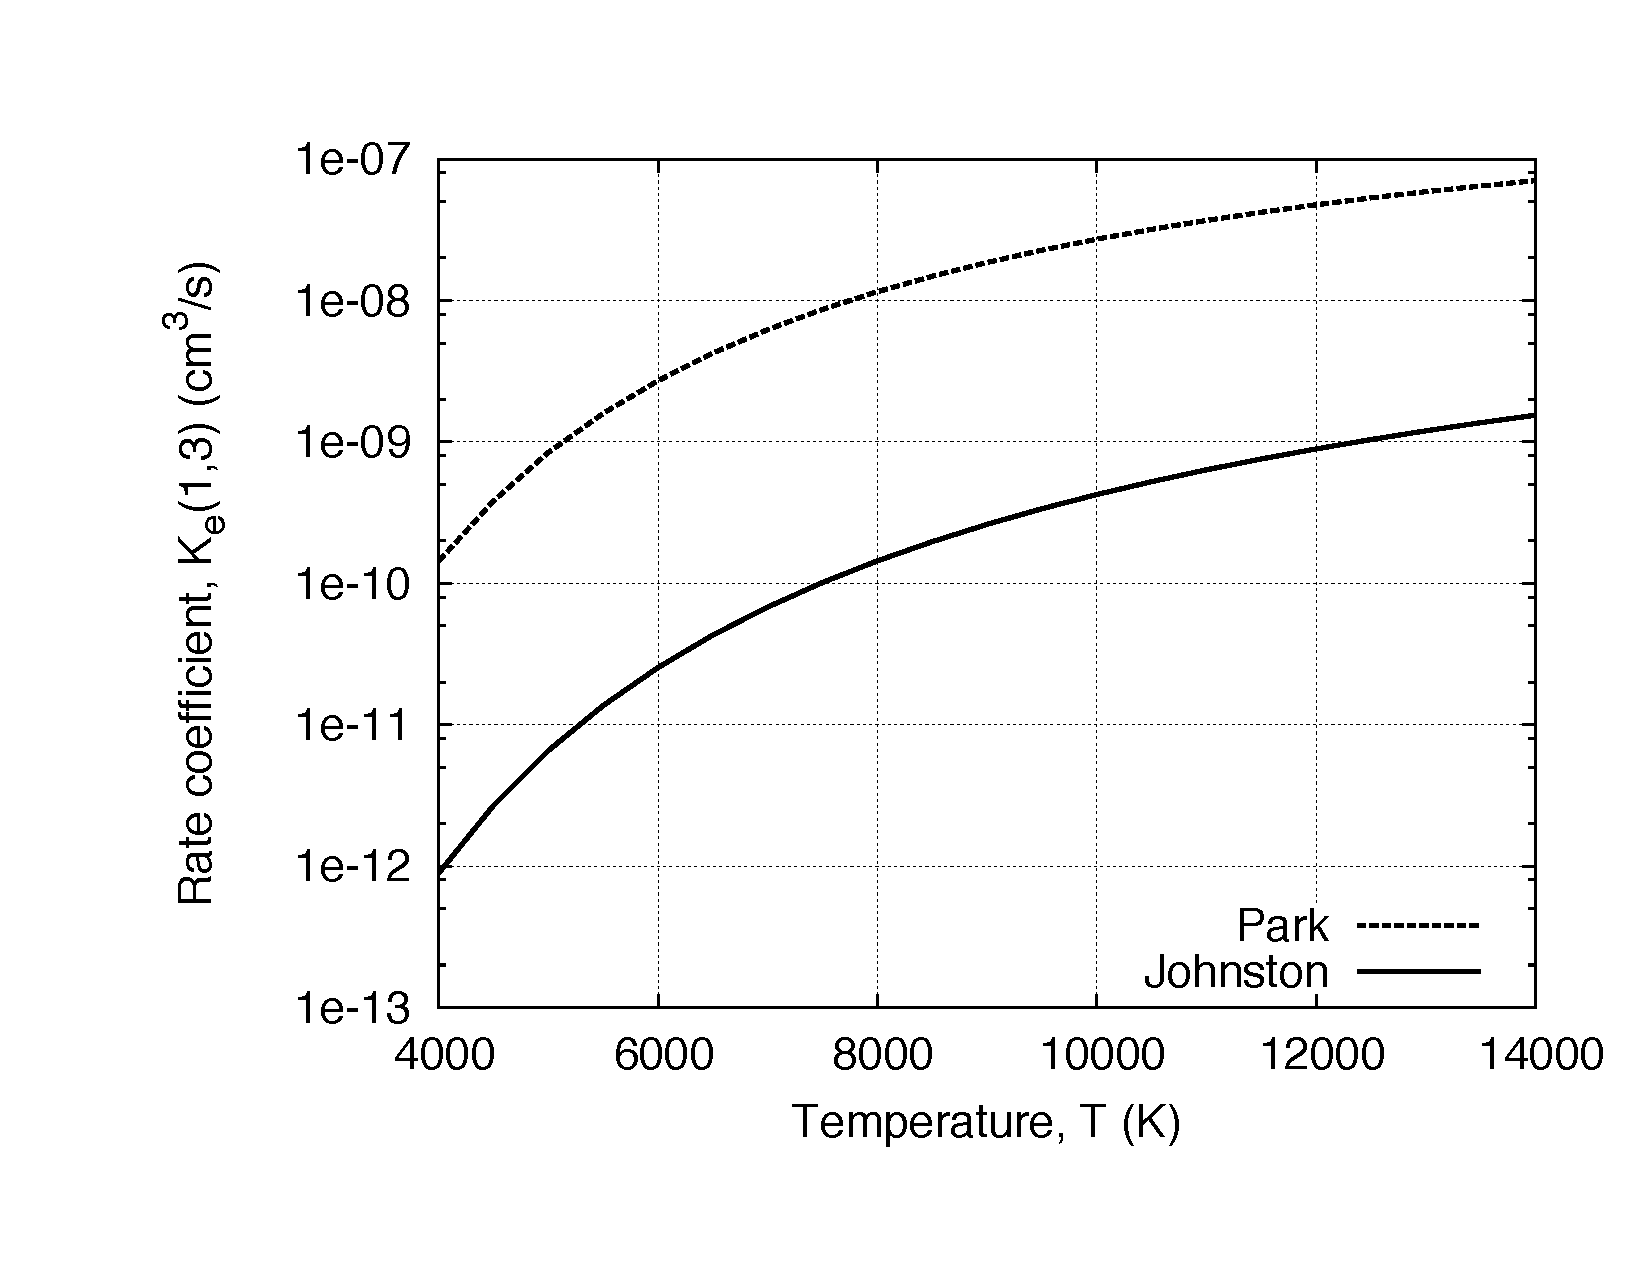
\includegraphics[width=0.48\linewidth]{collisional-radiative-modelling/figures/K_EIE_N2_plus_X_to_B.pdf} \label{fig:K_EIE_N2_plus_X_to_B}}
 \subfloat[$\NNplevA \Longrightarrow \NNplevB$]{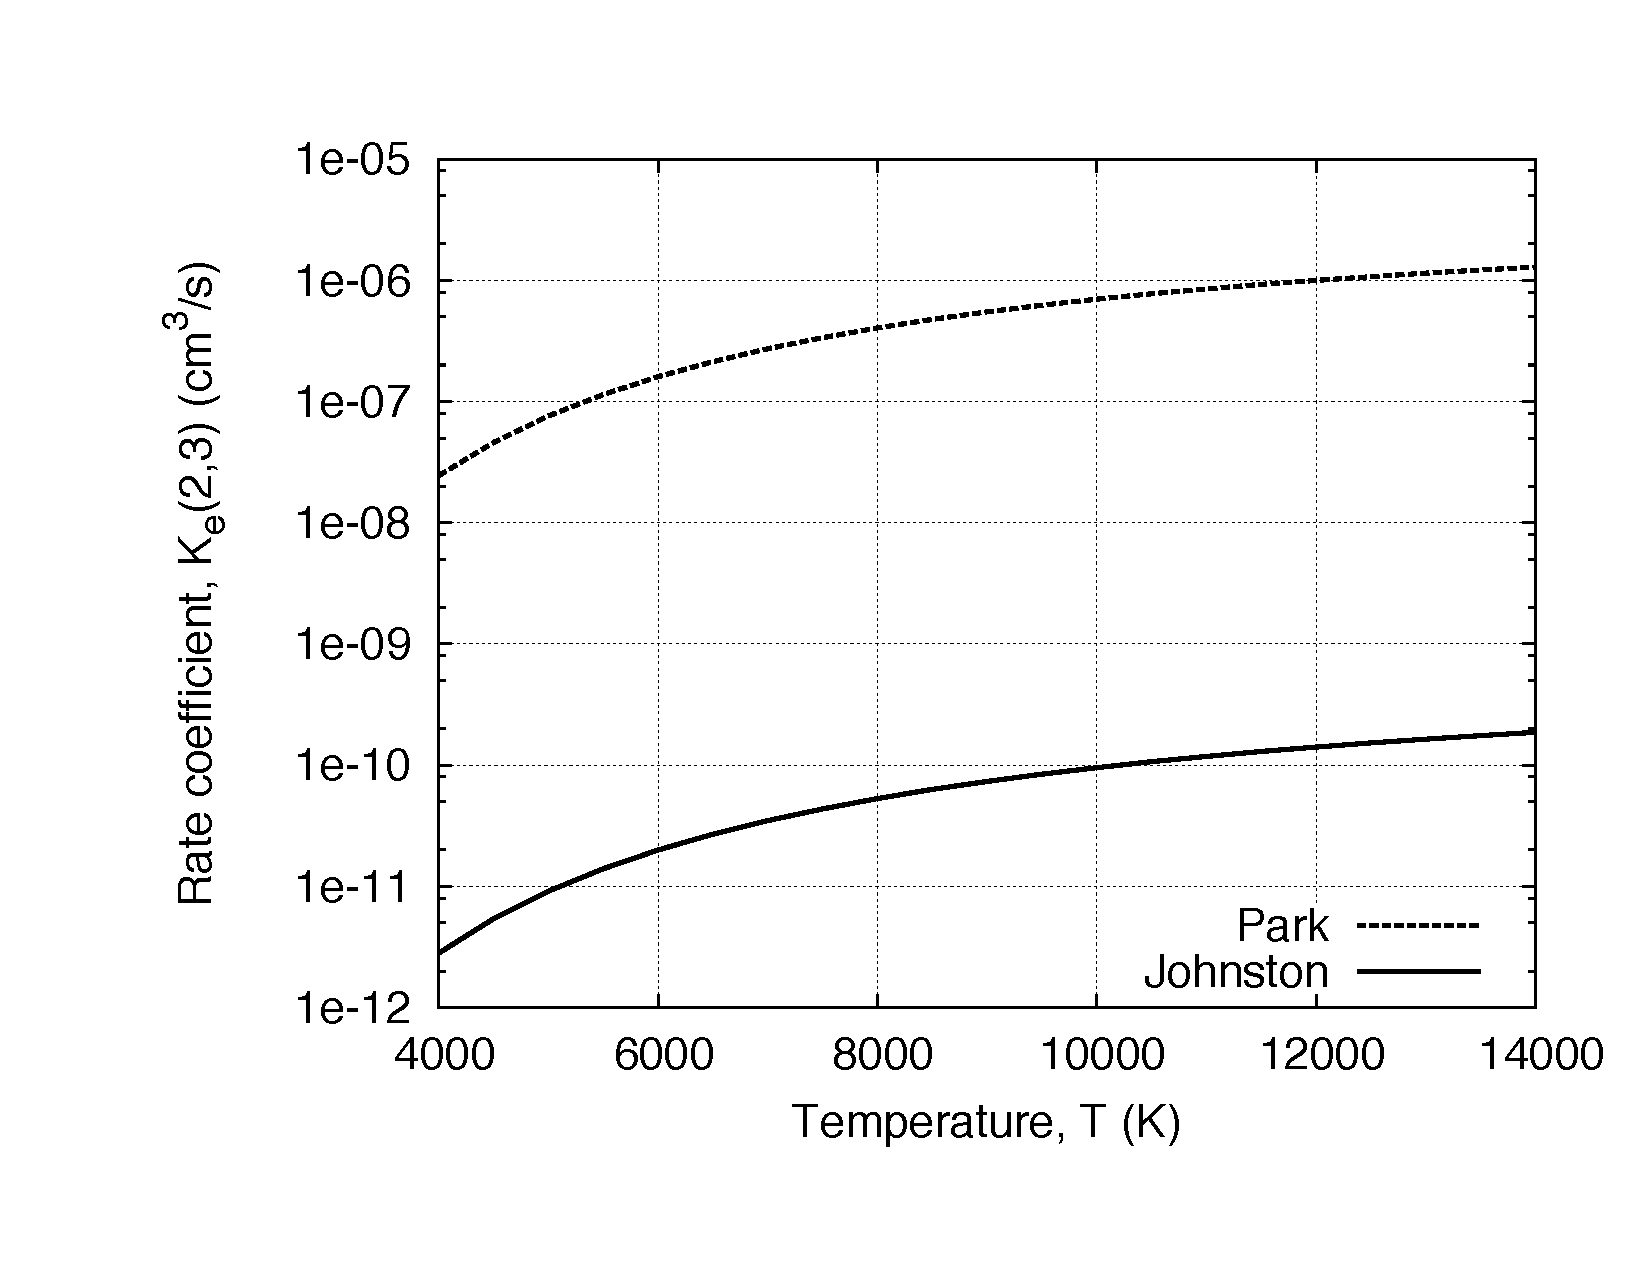
\includegraphics[width=0.48\linewidth]{collisional-radiative-modelling/figures/K_EIE_N2_plus_A_to_B.pdf} \label{fig:K_EIE_N2_plus_A_to_B}}
 \caption{Comparison of electron impact excitation rate coefficients for transitions to the $\NNplevB$ state of N$_2^+$.}
 \label{fig:K_EIE_N2_plus}
\end{figure}

\FloatBarrier

\subsection{Collisional-radiative model for CO$_2$--N$_2$--Ar mixtures}

 \begin{figure}[p]
 \centering
 \subfloat[Number density profile]{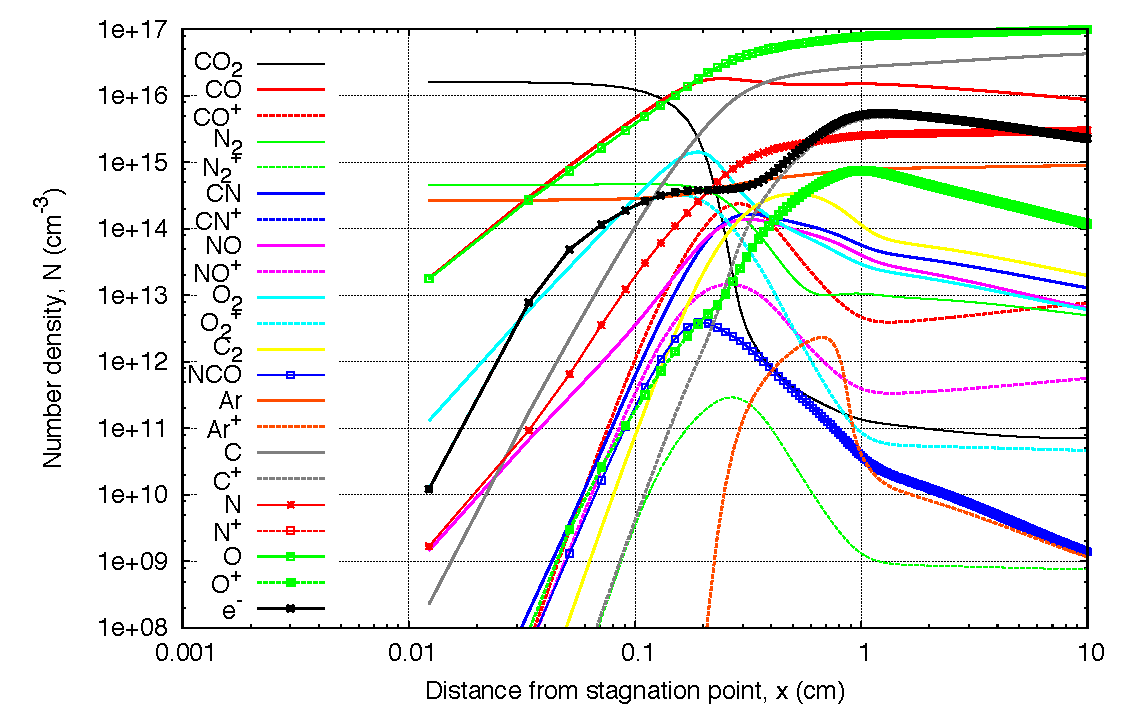
\includegraphics[width=0.9\linewidth]{collisional-radiative-modelling/figures/Mars_number_densities.pdf} \label{fig:Mars_number_densities}} \\
 \subfloat[Radiative emission profile]{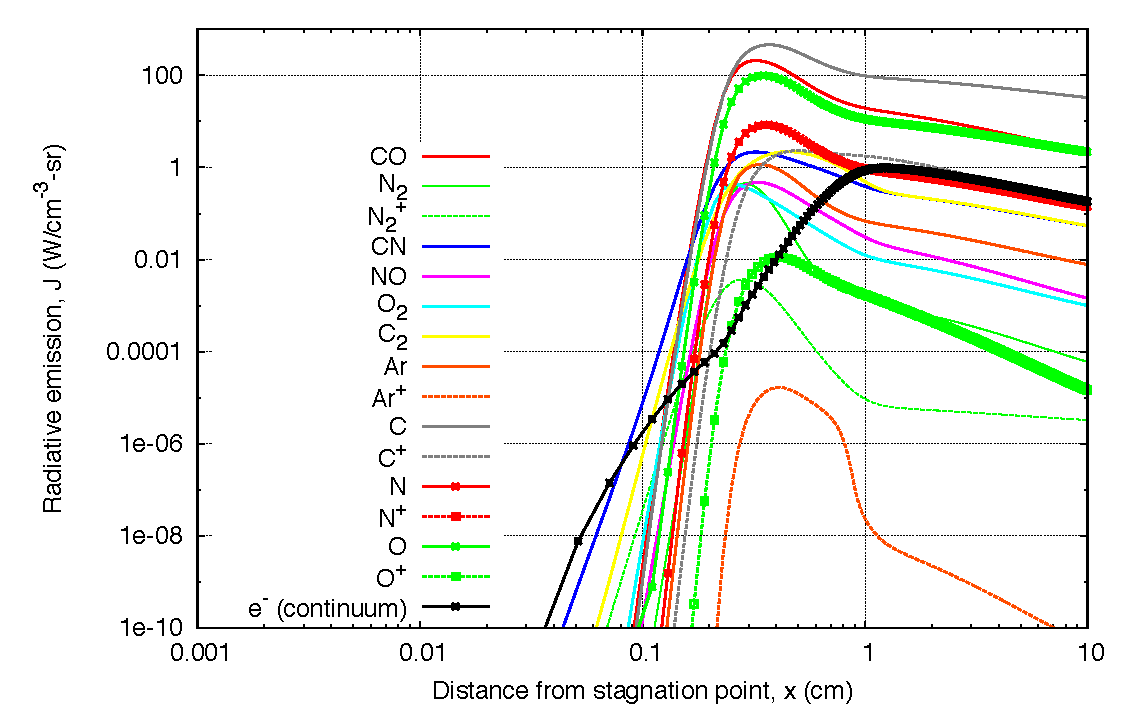
\includegraphics[width=0.9\linewidth]{collisional-radiative-modelling/figures/Mars_emissions.pdf} \label{fig:Mars_emissions}}
 \caption{Post-shock species number density and radiative emission profiles along the stagnation streamline for a hypothetical Mars aerocapture entry condition ($p_\infty = 6.2$\,Pa, $T_\infty = 161$\,K, $u_\infty = 9,440$\,m/s).}
\end{figure}

Figures~\ref{fig:Mars_number_densities} and~\ref{fig:Mars_emissions} present post-shock species number density and radiative emission profiles respectively for a hypothetical high-speed Mars aerocapture condition from the trajectory study of Braun \textit{et al.}~\cite{BPH90}.
The condition corresponds to that predicted for an aerocapture vehicle with nose radius 10\,m at 44.9\,km altitude that entered the Martian atmosphere at 9.79\,km/s.
This point is just prior to peak heating and is characterised by very strong thermochemical nonequilibrium.
Behind the shock CO$_2$ and N$_2$ quickly dissociate, forming an initial pool of CO and N$_2$ molecules and C, N and O atoms that allow exchange reactions to begin.
At 1\,mm behind the shock reactions have only just begun to occur and CN and C$_2$ systems and continuum transitions dominate the radiative emission.
By 3\,mm behind the shock dissociation is essentially complete and peak emission occurs, with atomic C lines, the VUV CO band systems and atomic O lines contributing 99\% of the radiative emission.
At peak emission the next strongest radiators are N, CN, C$_2$ and Ar, however their emission strength is on average two orders of magnitude less than CO and C.
As equilibrium is approached the total radiation drops by an order of magnitude, C, CO and O (in that order) continue to dominate the radiative emission while the relative strength of the continuum transitions increases due to the growing free electron population.
The free electron mole-fraction between peak-emission and chemical equilibrium is in the order of $10^{-2}$.

\par

Although C, CO and O are by far the strongest radiators when Boltzmann level populations is assumed, the nonequilibrium emission is likely to be significantly less due to radiative depletion of the high lying states.  
Therefore in the present work we chose to apply the collisional-radiative model to all the significant radiators -- C, CO, O, C$_2$, N, Ar and CN.
Although the free electron number density is lower than for Earth re-entry, electron impact collisional processes should still dominate over heavy particle collisions due to their high efficiency.
Thus in the present work only electron impact collisional processes will be considered.

\subsubsection{Atomic species: Ar, C, N and O}

Table~\ref{tab:Ar-C-N-O-CR} summarises the implemented rate coefficients for the collisional-radiative mechanisms considered for atomic species in CO$_2$--N$_2$--Ar mixtures.
Similarly as for N$_2$--O$_2$ mixtures, the collisional mechanisms considered for atoms are electron impact excitation and ionisation, and the radiative processes considered are bound-bound optically allowed transitions.
As the Drawin~\cite{drawin_1968} cross sections have been shown to be appropriate for calculating non-Boltzmann emission from atomic argon~\cite{Vlcek1989, BGV1998}, the Drawin model proposed by Panesi~\cite{panesi_phd} is applied to calculate electron impact excitation and ionisation of Ar.
For atomic carbon, accurate rate-coefficients are obtained from Suno and Kato~\cite{SK2006} for electron impact excitation and ionisation of the ground and metastable states.
The remaining transitions described by the semi-empirical model of Gryzinski~\cite{Gryz59}.
The collisional-radiative models selected for N and O in N$_2$--O$_2$ mixtures are retained here for application to CO$_2$--N$_2$--Ar mixtures.
All radiative transition probabilities $A(i,j)$ are calculated using Equation~\ref{eq:A_av} where the individual line transition probabilities are obtained from the NIST Atomic Species Database~\cite{NIST_ASD} (see Table~\ref{tab:atomic-lines}).

\begin{table}[bht]
 \center
 \caption{Summary of the collisional-radiative mechanisms implemented for Ar, C, N and O in CO$_2$--N$_2$--Ar mixtures.}
 \label{tab:Ar-C-N-O-CR}
 \begin{tabular*}{1.0\textwidth}{cccc}
  \hline Species                         & Electronic levels & CR mechanisms                                & Models    \\
  \hline  
                  Ar                               & All & Electron impact excitation                & Drawin (Reference~\cite{panesi_phd}) \\
                                                     &       & Electron impact ionisation               &  Drawin (Reference~\cite{panesi_phd}) \\
                                                     &       & Radiative decay                                 & NIST Atomic Spectra Database~\cite{NIST_ASD} \\
                  C                                & All & Electron impact excitation                & (a) Suno and Kato~\cite{SK2006} \\
                                                     &       &                                                               & (b) Gryzinski~\cite{Gryz59} \\
                                                     &       & Electron impact ionisation               & (a) Suno and Kato~\cite{SK2006} \\
                                                     &       &                                                               & (b) Drawin (Reference~\cite{panesi_phd}) \\
                                                     &       & Radiative decay                                 & NIST Atomic Spectra Database~\cite{NIST_ASD} \\    
                  N                                & All & Electron impact excitation                & (a) Frost \textit{et al.}~\cite{FAS+1998} \\
                                                     &       &                                                               & (b) Gryzinski~\cite{Gryz59} \\
                                                     &       & Electron impact ionisation               & (a) Soon and Kunc~\cite{SK1990} \\
                                                     &       &                                                               & (b) Drawin (Reference~\cite{panesi_phd}) \\
                                                     &       & Radiative decay                                 & NIST Atomic Spectra Database~\cite{NIST_ASD} \\
                  O                                & All & Electron impact excitation                & (a) Zatsarinny and Tayal~\cite{ZT2003} \\
                                                     &       &                                                               & (b) Gryzinski~\cite{Gryz59} \\
                                                     &       & Electron impact ionisation               & (a) Soon and Kunc~\cite{SK1990} \\
                                                     &       &                                                               & (b) Drawin (Reference~\cite{panesi_phd}) \\
                                                     &       & Radiative decay                                 & NIST Atomic Spectra Database~\cite{NIST_ASD} \\                                   
  \hline
 \end{tabular*}
\end{table}


\subsubsection{(a) Electron impact excitation of C}


Suno and Kato~\cite{SK2006} compiled an extensive electron-impact ionisation, excitation and charge exchange cross section database for carbon atoms and ions.
Although the database extends to electron temperatures of 1\,keV as it is designed nuclear fusion applications, the presented electron impact excitation data for C is shown to agree well with the experimental data of Duneath \textit{et al.}~\cite{DFB+1997} and others obtained in the 1\,eV electron temperature range of present interest.
The data are presented as curve fits for the collision strength $\Omega_{ij}$ from which the rate coefficient can be calculated as:

\begin{equation}
 K_e(i,j) = \frac{8.010 \times 10^{-8}}{\omega_i \sqrt{T_e}} y \int_1^\infty \Omega_{ij} e^{-y X} dX 
\end{equation}

\noindent where $T_e$ is in eV, $y = \Delta E_{ij} / T_e$ and $X = E_e / \Delta E_{ij}$.

\par

Figure~\ref{fig:K_EIE_C} compares the electron impact excitation rate coefficient for various transitions of C.
For all transitions except excitation of the ground to first excited state (see Figure~\ref{fig:K_EIE_C_1_to_2}}), the Suno and Kato rates are between 2 and 1000 times larger than the rates predicted by the approximate models.
This is in contrast to the electron impact excitation rates of N and O, where the accurate rates for low lying levels was bounded by the approximate models.
It is therefore possible that the rates of Suno and Kato are not suitable for the temperature range considered.
In the absence of better electron impact excitation data, however, the Suno and Kato rates are preferenced for transitions from low lying states while the Gryzinski model is applied to the remaining transitions.

\begin{figure}[p]
 \centering
 \subfloat[$\Clevone \Rightarrow \Clevtwo$ (Forbidden)]{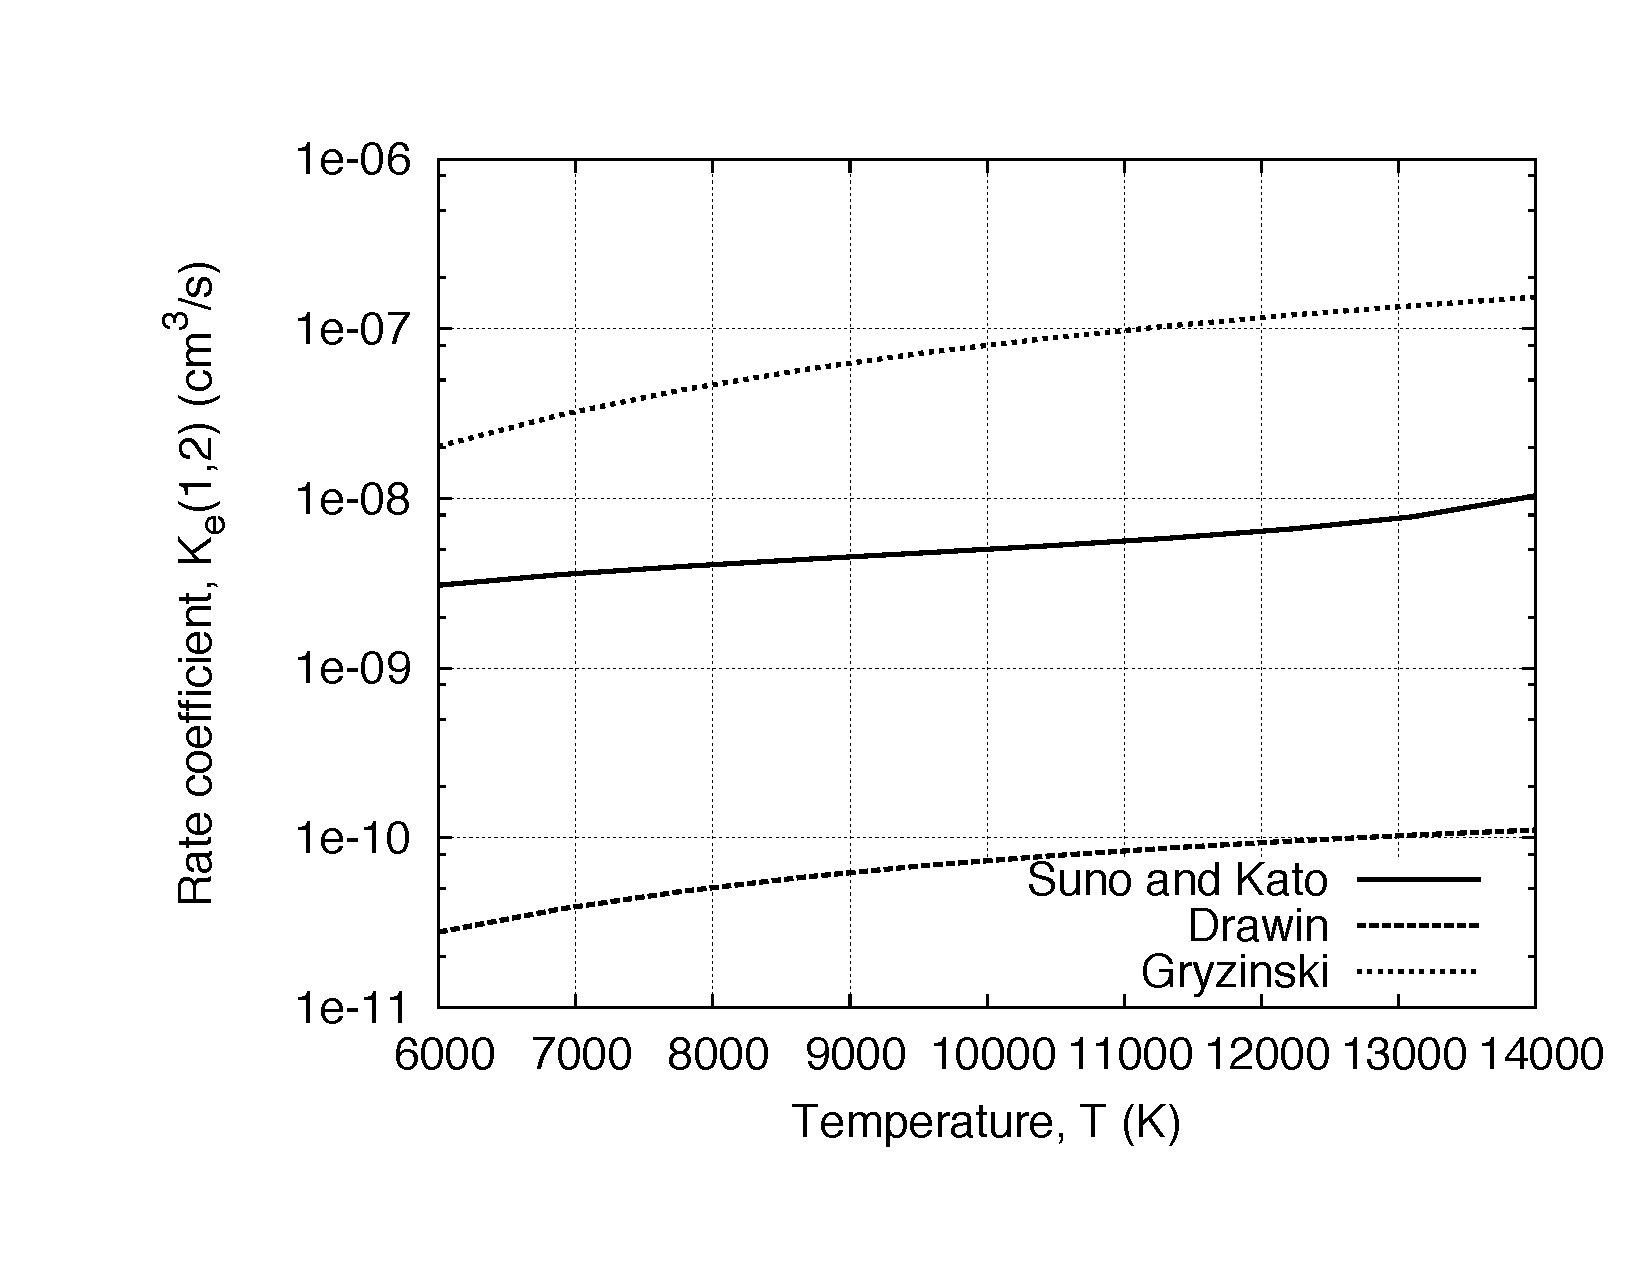
\includegraphics[width=0.48\linewidth]{collisional-radiative-modelling/figures/K_EIE_C_1_to_2.pdf} \label{fig:K_EIE_C_1_to_2}}
 \subfloat[$\Clevtwo \Rightarrow \Clevthree$ (Forbidden)]{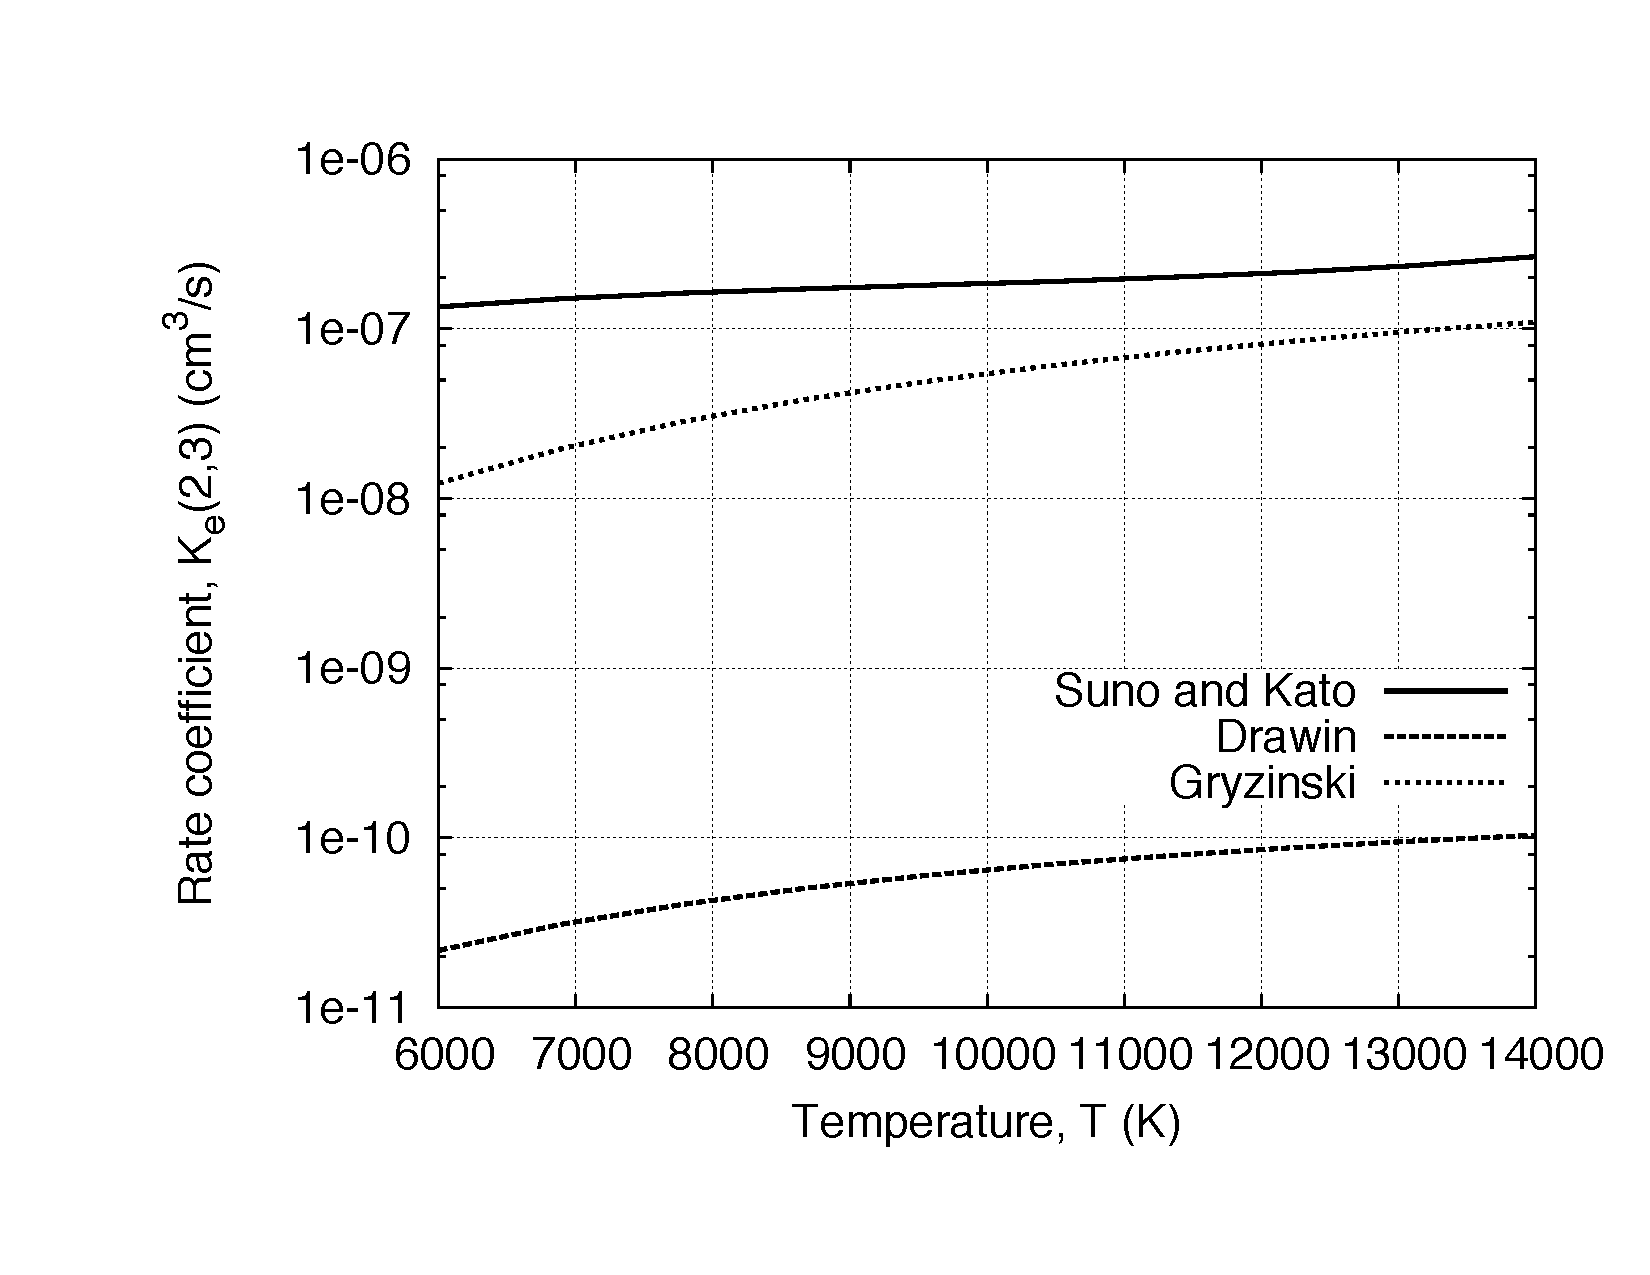
\includegraphics[width=0.48\linewidth]{collisional-radiative-modelling/figures/K_EIE_C_2_to_3.pdf} \label{fig:K_EIE_C_2_to_3}} \\
 \subfloat[$\Clevone \Rightarrow \Clevfive$ (Allowed)]{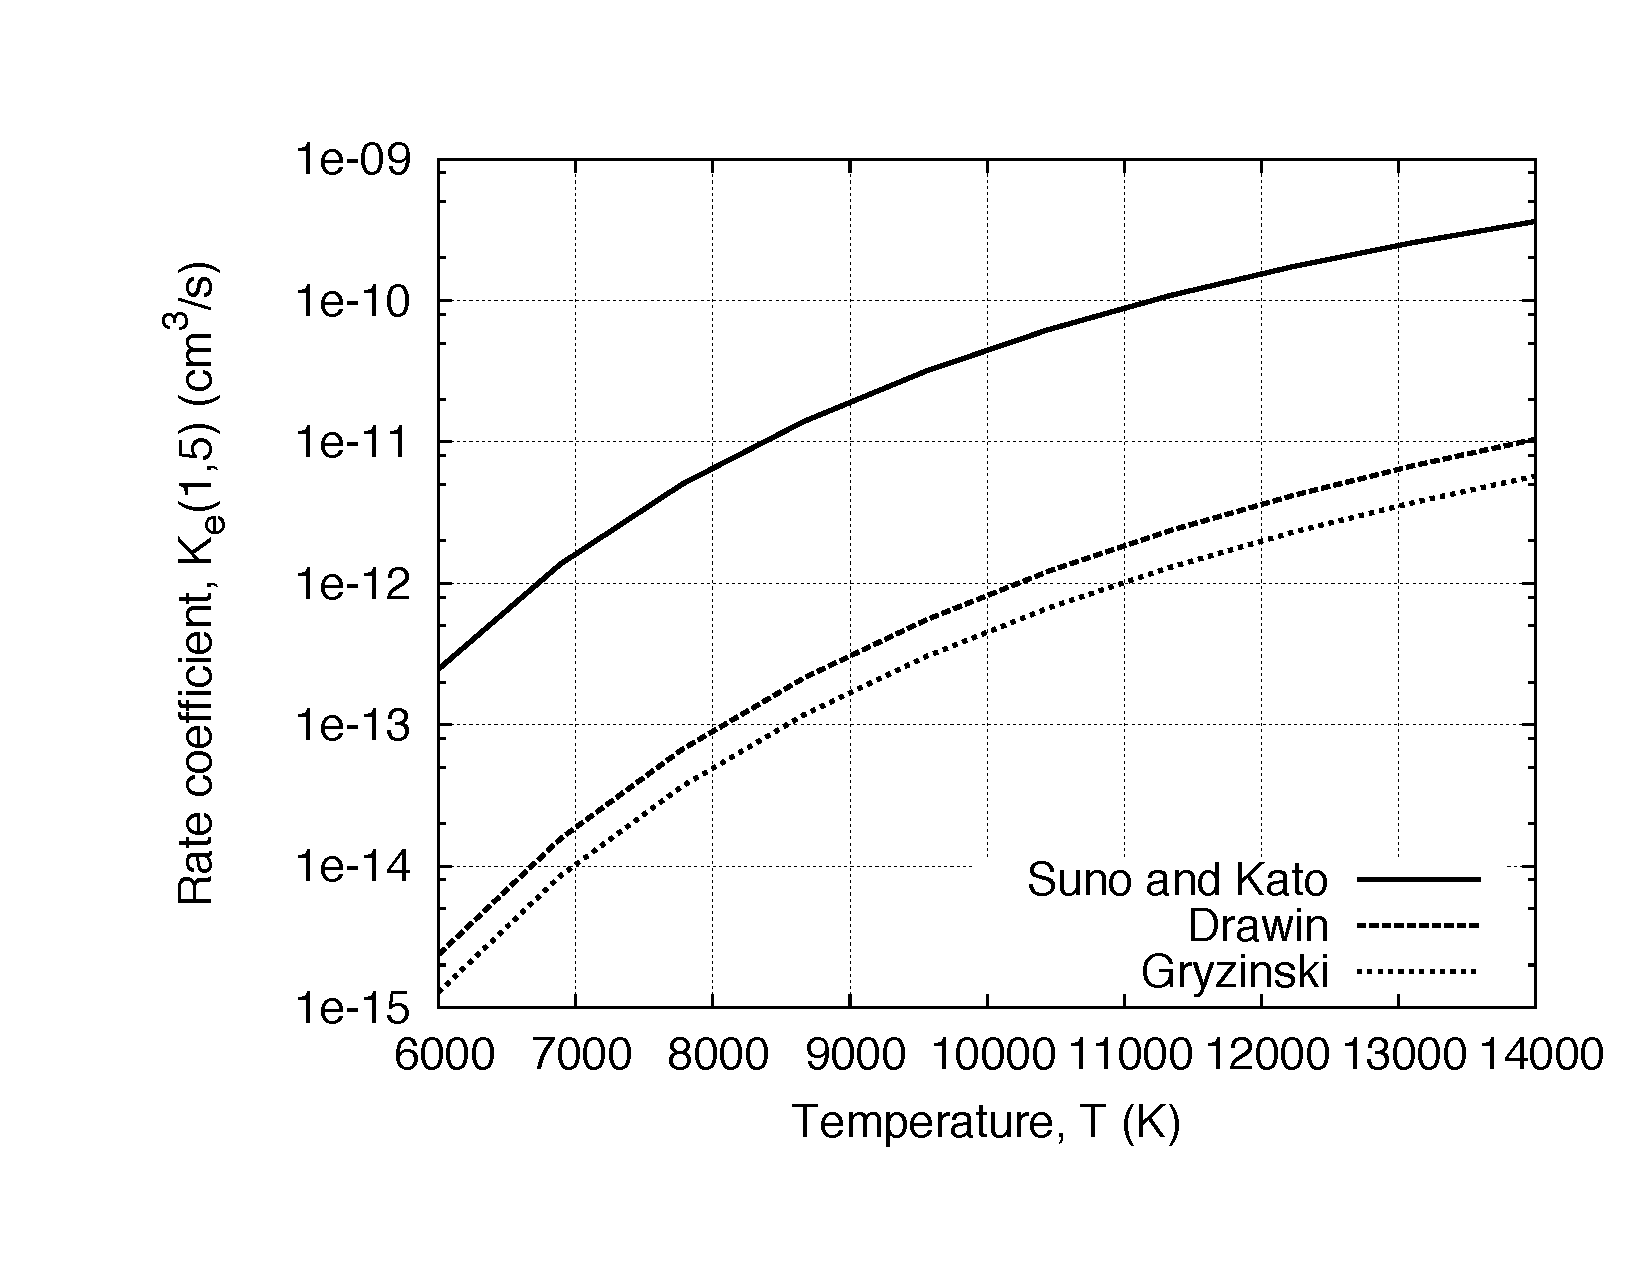
\includegraphics[width=0.48\linewidth]{collisional-radiative-modelling/figures/K_EIE_C_1_to_5.pdf} \label{fig:K_EIE_C_1_to_5}}
 \subfloat[$\Clevtwo \Rightarrow \Clevfive$ (Forbidden)]{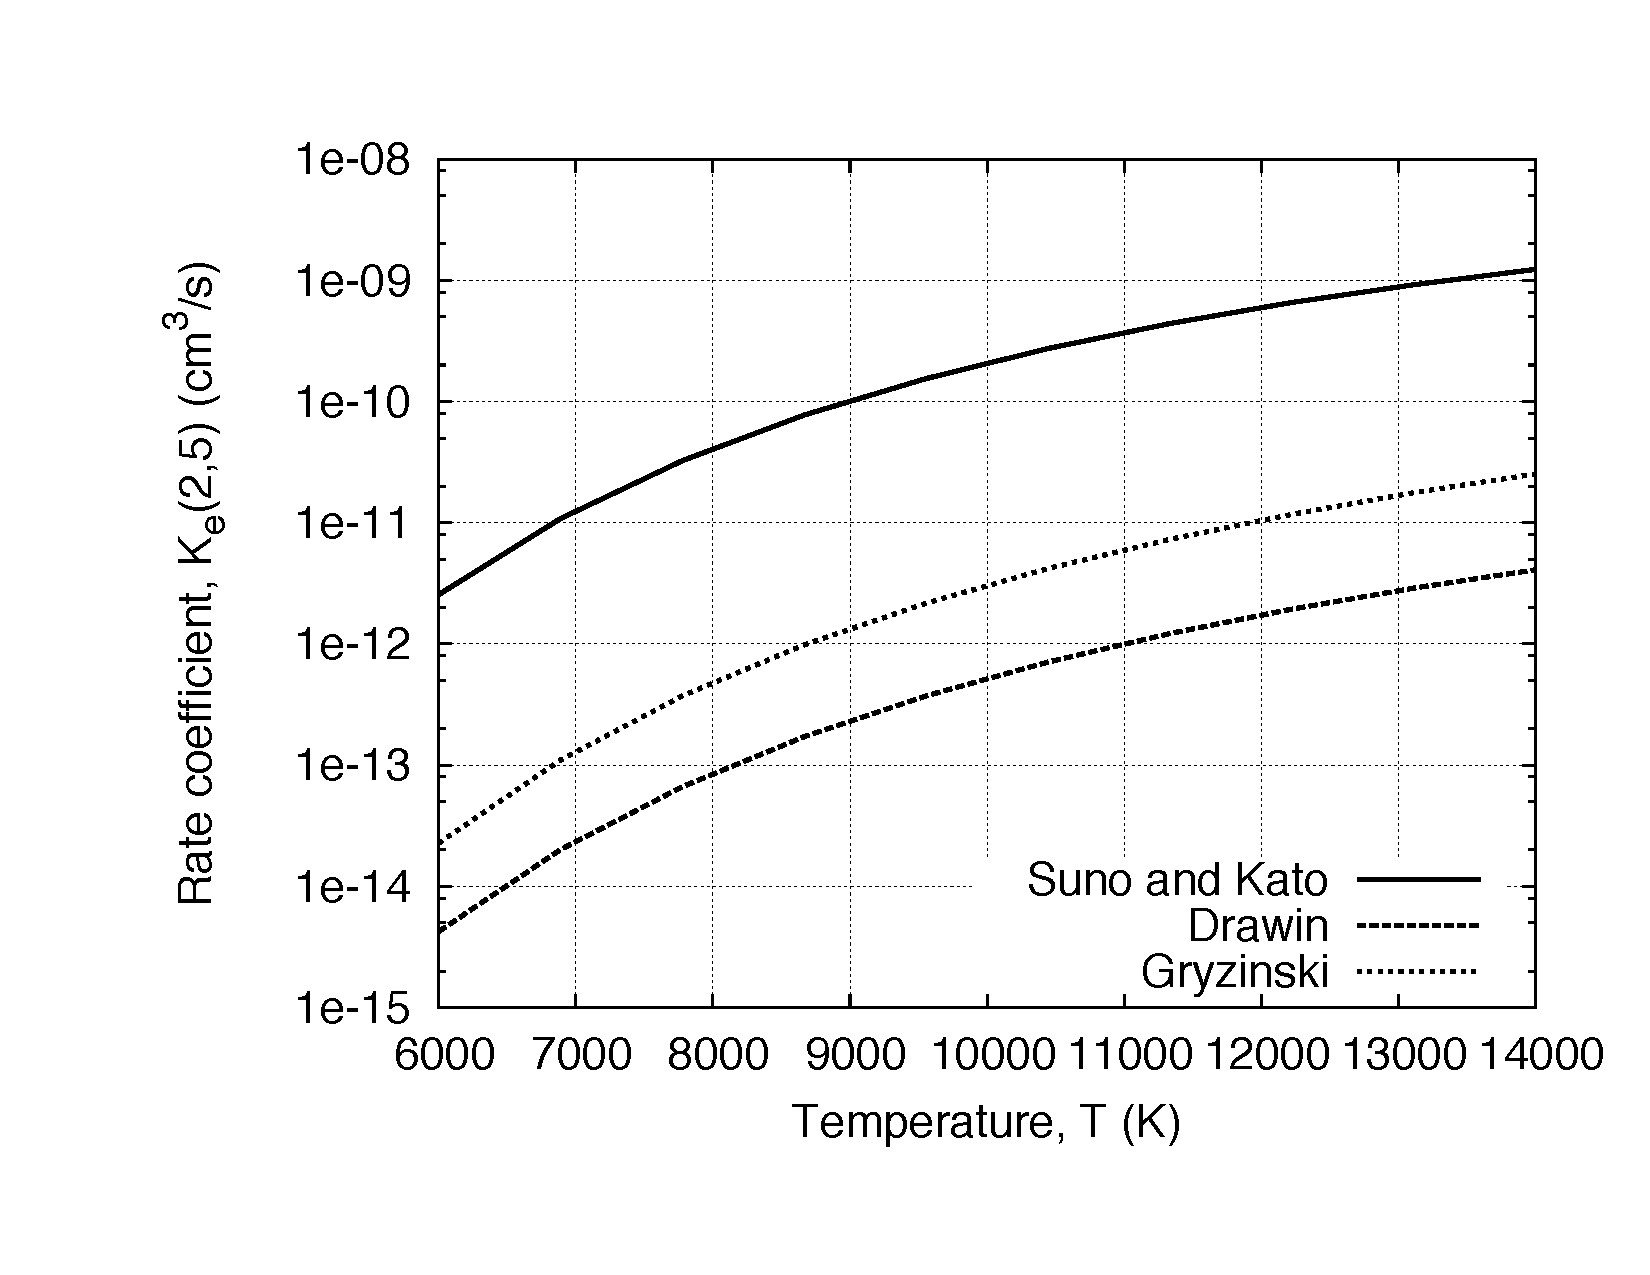
\includegraphics[width=0.48\linewidth]{collisional-radiative-modelling/figures/K_EIE_C_2_to_5.pdf} \label{fig:K_EIE_C_2_to_5}} \\
 \subfloat[$\Clevone \Rightarrow \Clevfifteen$ (Forbidden)]{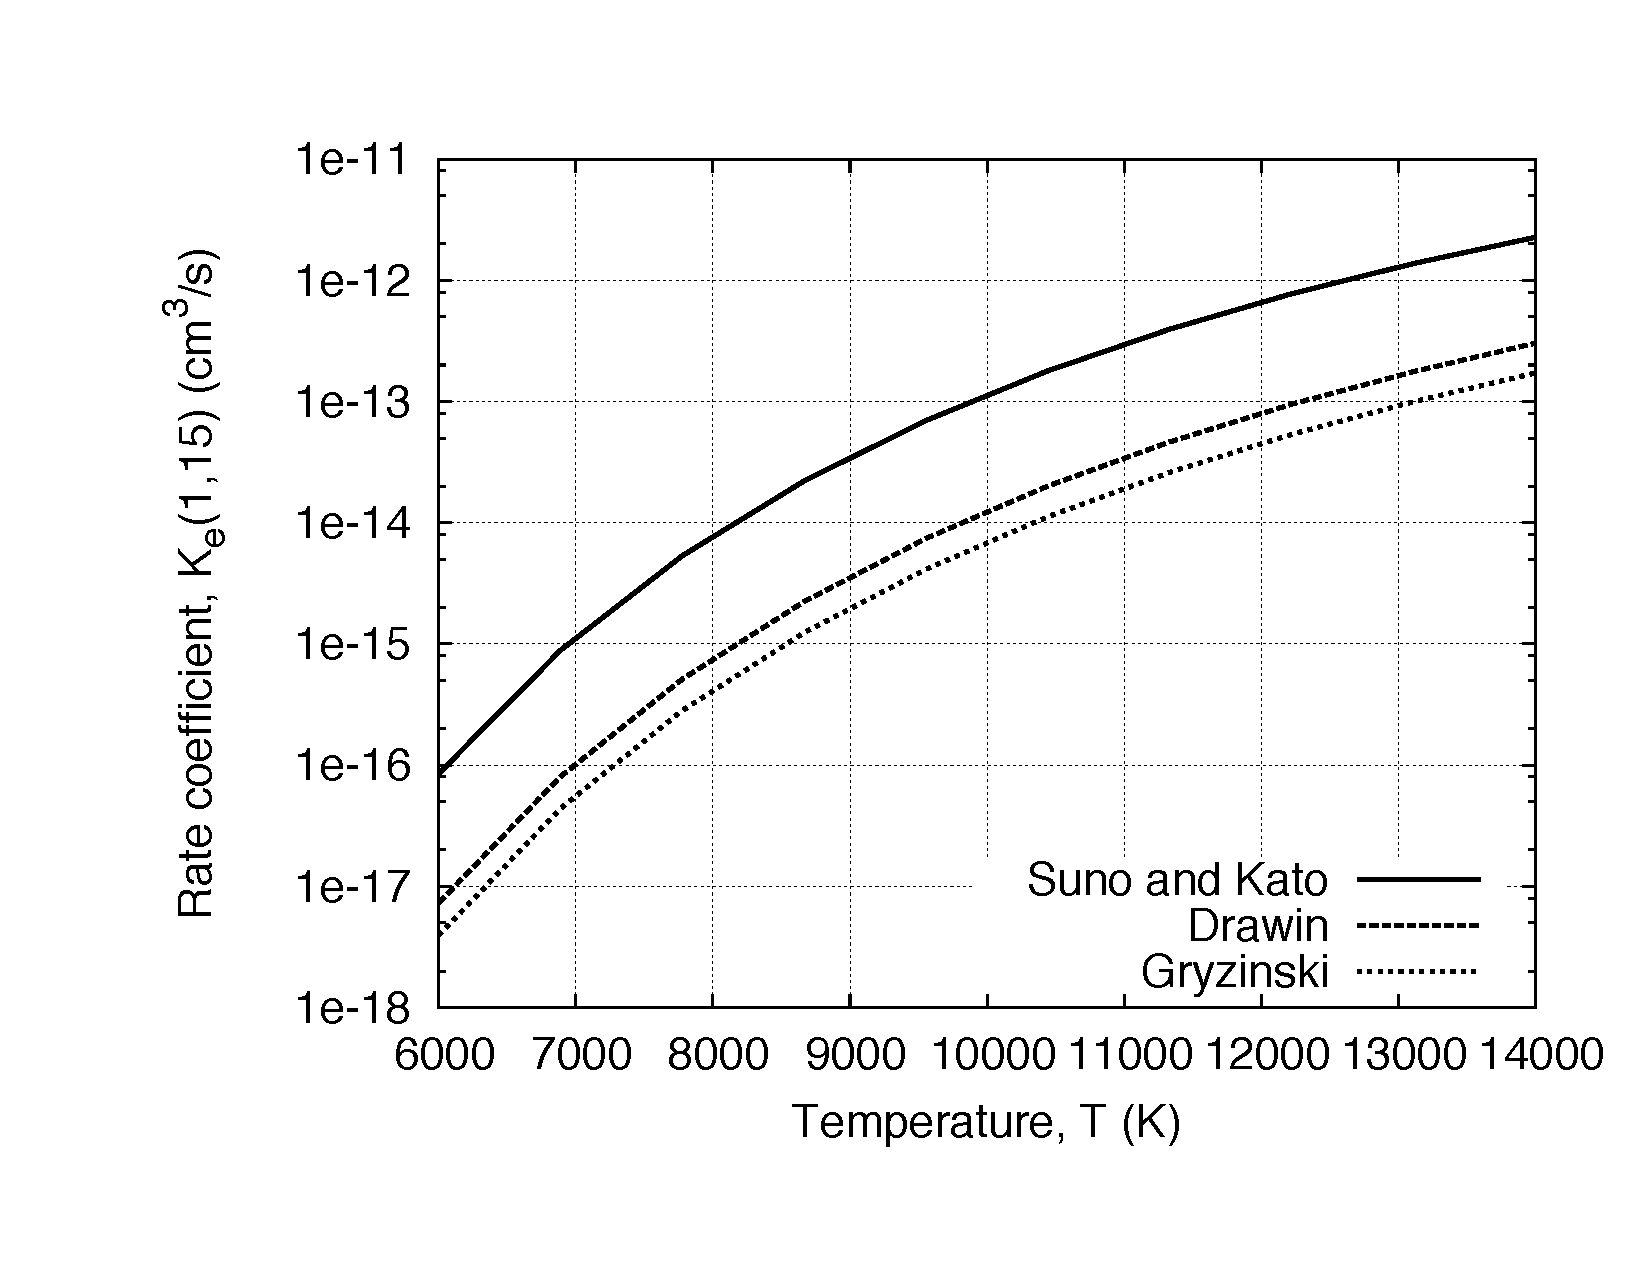
\includegraphics[width=0.48\linewidth]{collisional-radiative-modelling/figures/K_EIE_C_1_to_15.pdf} \label{fig:K_EIE_C_1_to_15}}
 \subfloat[$\Clevone \Rightarrow \Cleveighteen$ (Allowed)]{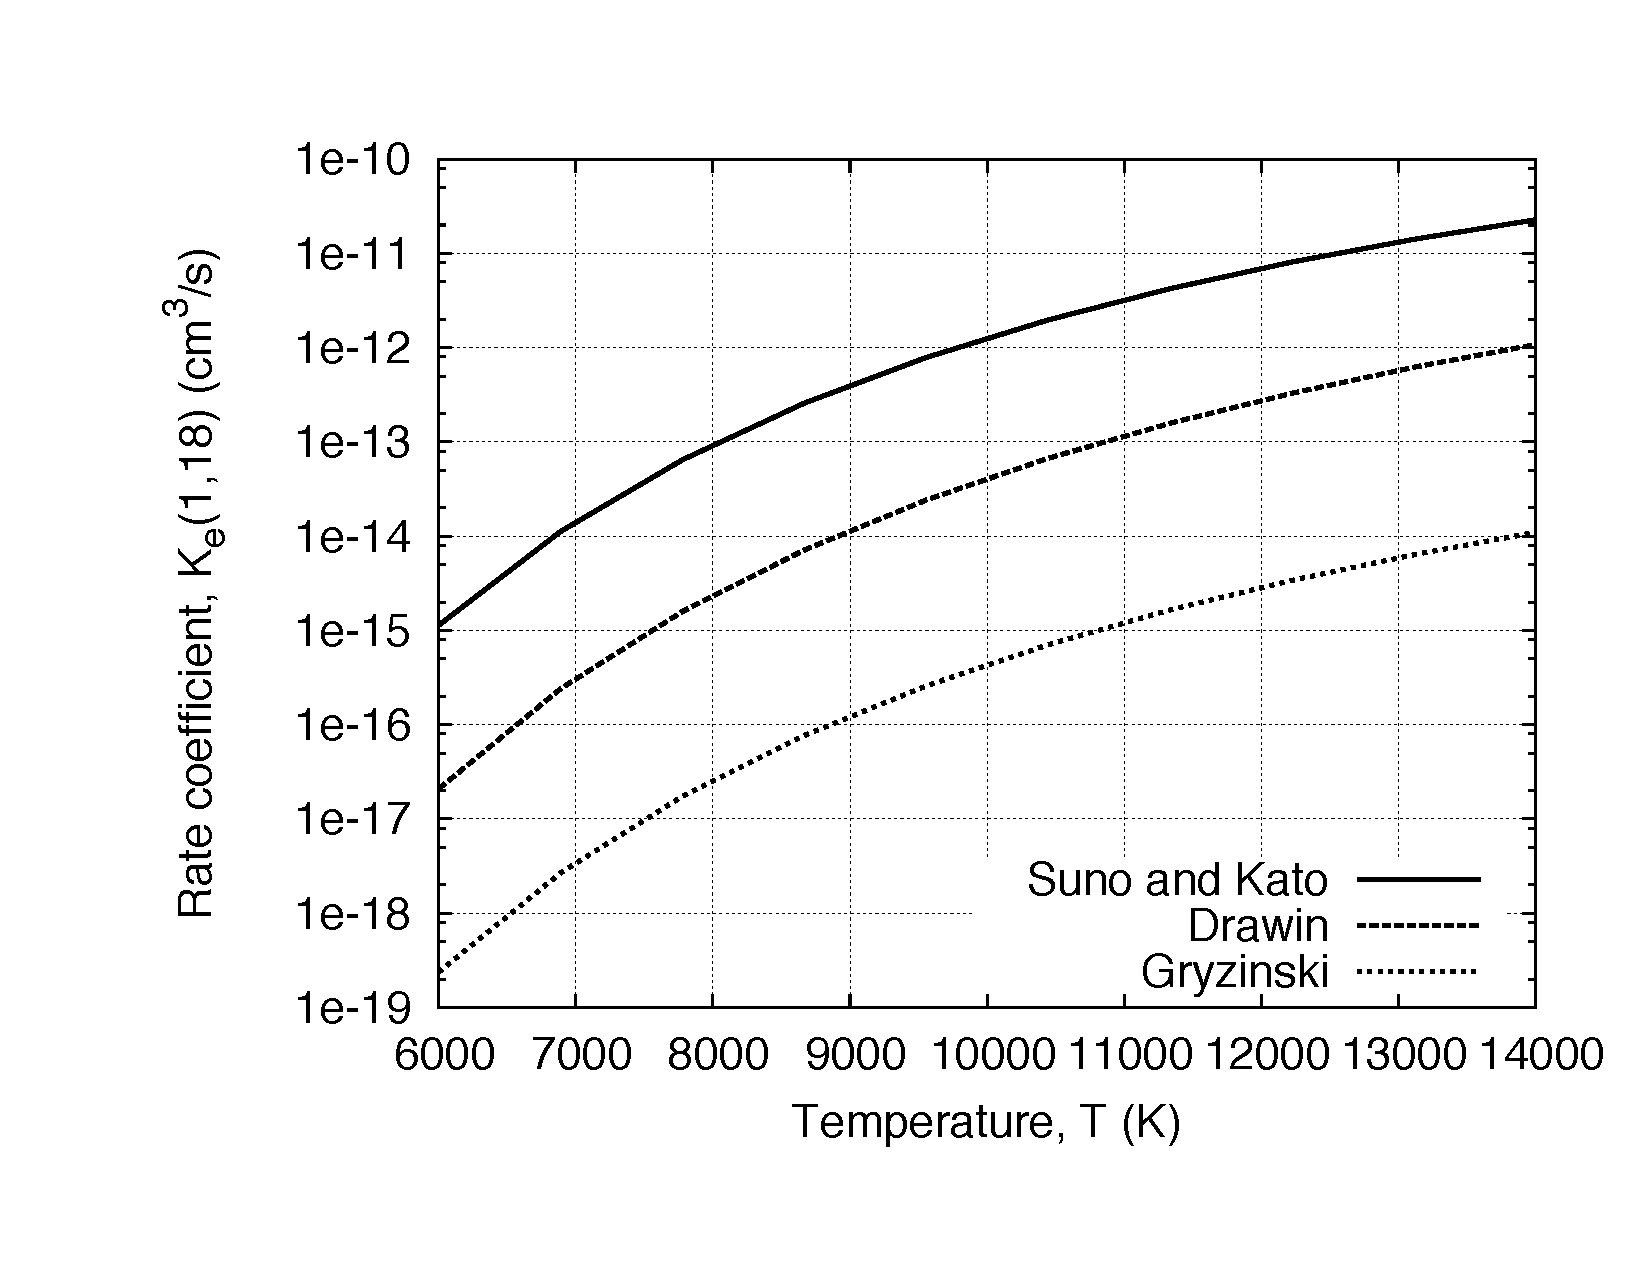
\includegraphics[width=0.48\linewidth]{collisional-radiative-modelling/figures/K_EIE_C_1_to_18.pdf} \label{fig:K_EIE_C_1_to_18}}
 \caption{Comparison of  electron impact excitation rate coefficients for atomic carbon.}
 \label{fig:K_EIE_O}
\end{figure}
%
\begin{figure}[!t]
 \centering
 \ContinuedFloat
  \subfloat[$\Clevone \Rightarrow \Clevtwenty$ (Forbidden)]{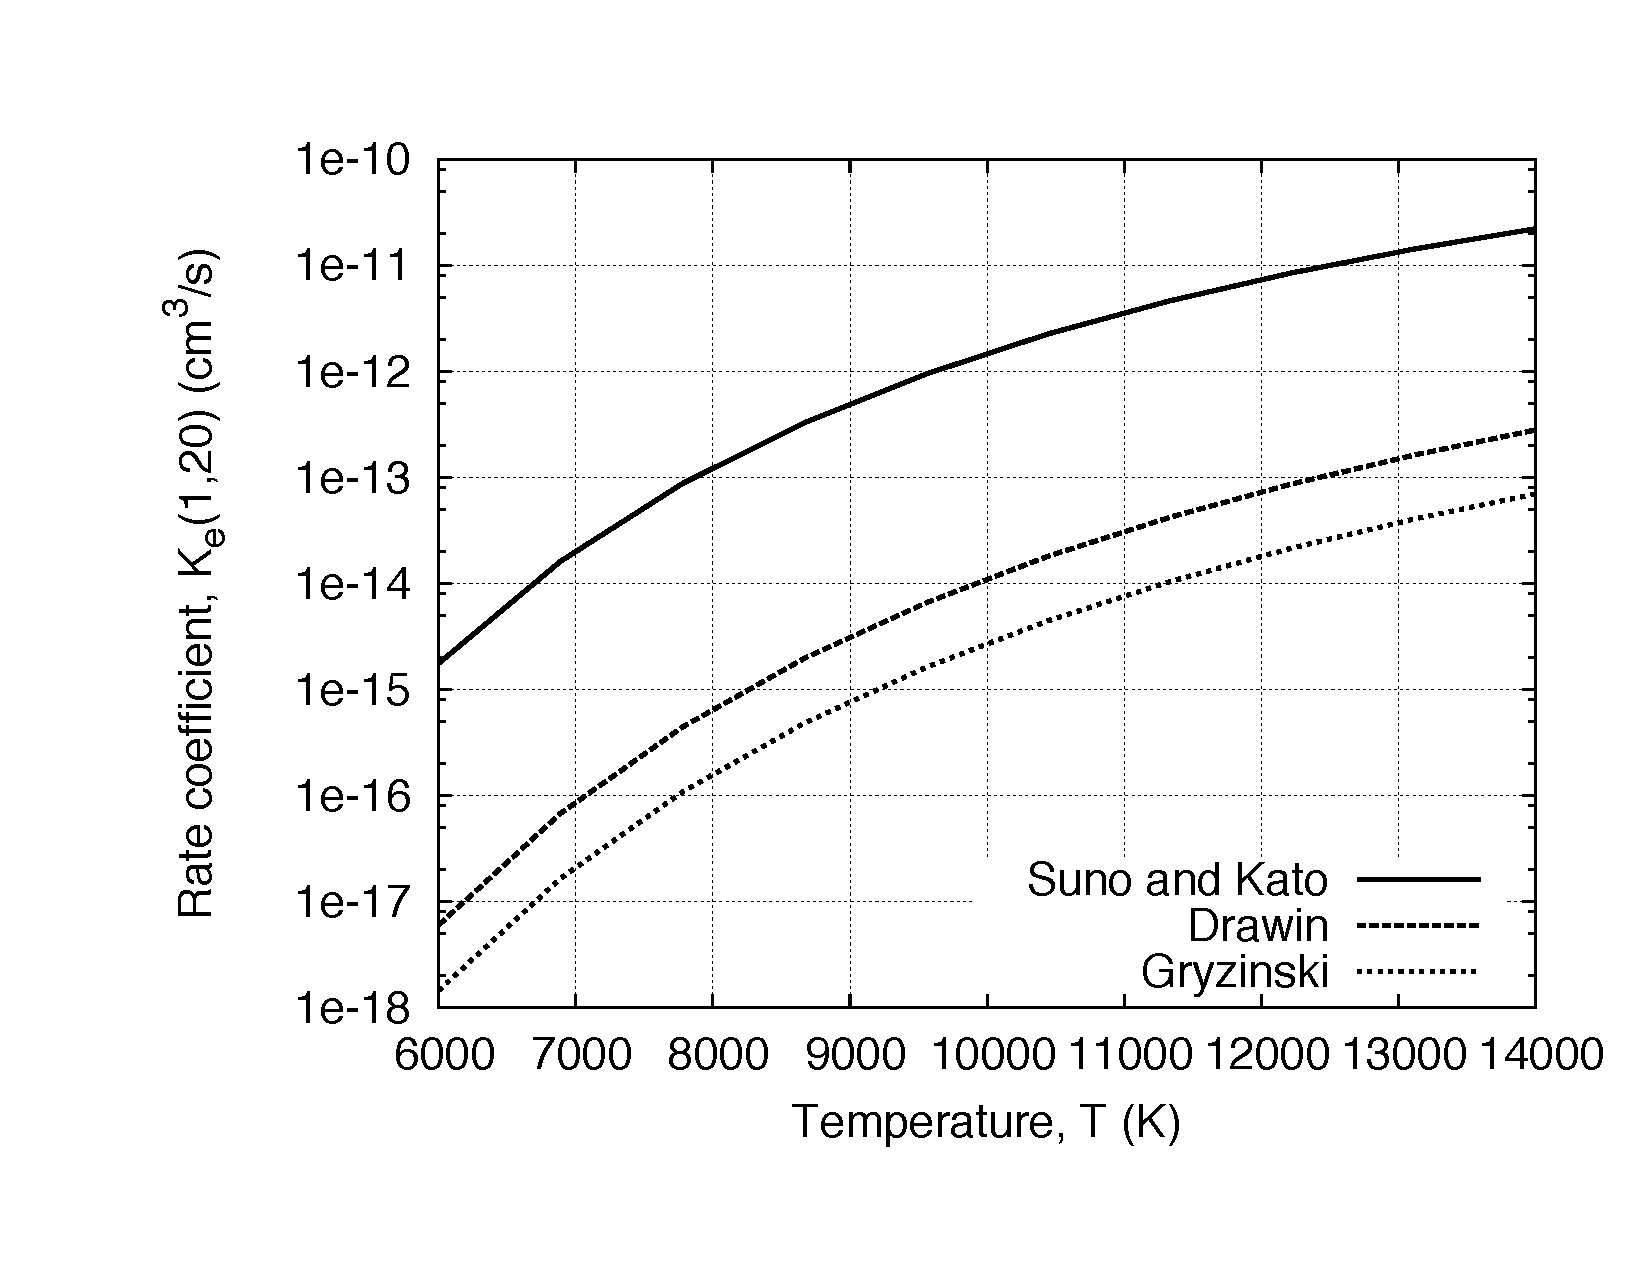
\includegraphics[width=0.48\linewidth]{collisional-radiative-modelling/figures/K_EIE_C_1_to_20.pdf} \label{fig:K_EIE_C_1_to_20}} 
  \subfloat[$\Clevone \Rightarrow \Clevtwentytwo$ (Allowed)]{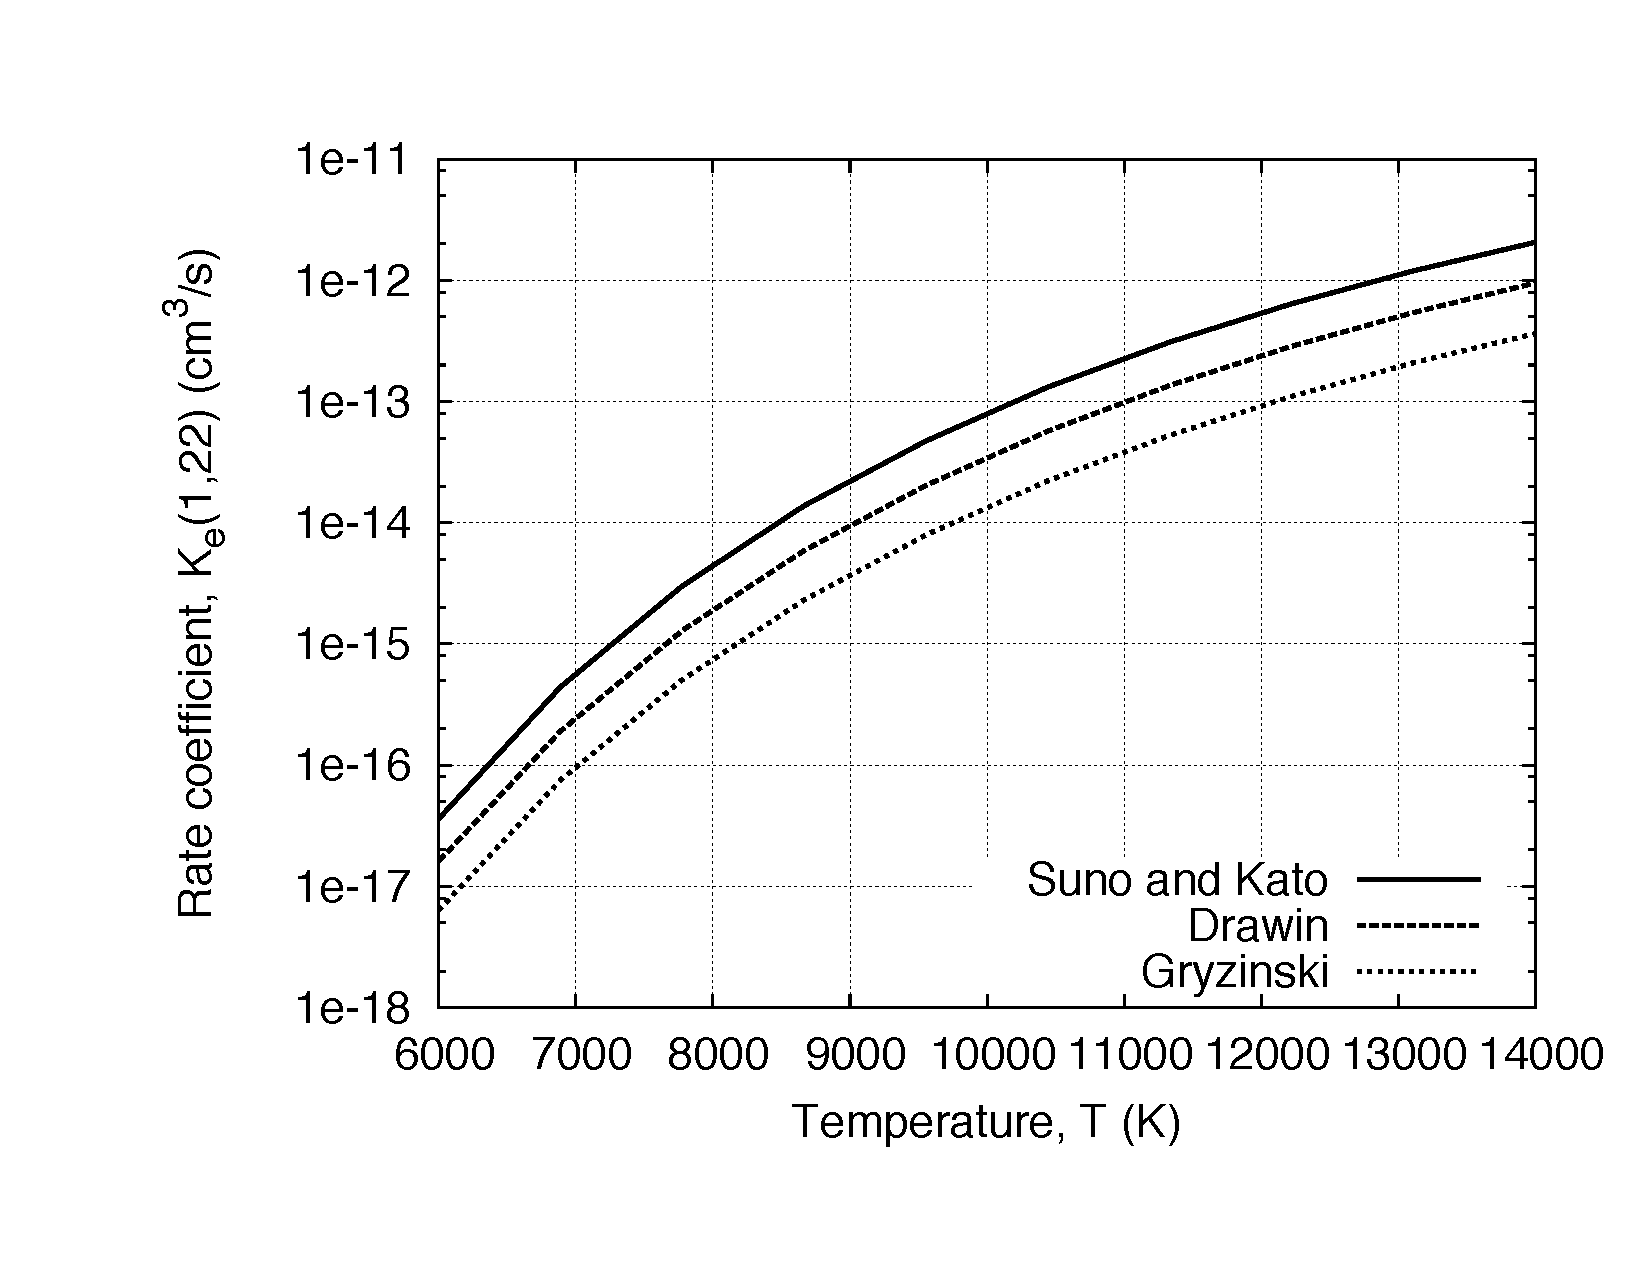
\includegraphics[width=0.48\linewidth]{collisional-radiative-modelling/figures/K_EIE_C_1_to_22.pdf} \label{fig:K_EIE_C_1_to_22}} 
 \caption{\textit{(Continued)} Comparison of  electron impact excitation rate coefficients for atomic carbon.}
 \label{fig:K_EIE_C}
\end{figure}

\subsubsection{(b) Electron impact ionisation of C}

Suno and Kato~\cite{SK2006} present the electron impact ionisation cross section for the ground state of atomic carbon in the following form:

\begin{equation}
 \sigma = \frac{1 \times 10^{-13}}{I E} \left \lbrace A_1 \text{ln} \left ( E / I \right ) + \sum_{j=2}^{N_A} A_j \left ( 1 - \frac{I}{E} \right )^{j-1} \right \rbrace \label{eq:SK_EII_CS}
\end{equation}

\noindent where $I$ and $E$ are the ionisation and electron energy in eV and $A_j$ are fitting coefficients.
The fitting coefficients have been selected to match the experimental measurements of Brook \textit{et al.}~\cite{BHS1978}.
Unfortunately Brook considered electron energies in the range $ 7 \leq E \leq 1000$\,eV, which is outside the $E \approx 1$\,eV range of present interest.
In the absence of electron impact ionisation cross sections for the metastable state of atomic carbon, in the present work Equation~\ref{eq:SK_EII_CS} is applied where $I$ is taken as the level-specific ionisation potential.
The rate coefficient is then calculated as:

\begin{equation}
 K_e(i,c) = \frac{8.010 \times 10^{-8}}{g_i \sqrt{T_e}} y \int_1^\infty \Omega_i e^{-y X} dX 
\end{equation}

\noindent where $T_e$ is in eV, $y = I / T_e$, $X = E_e / I$ and collision strength $\Omega_i$ for level $i$ is obtained from the cross section in Equation~\ref{eq:SK_EII_CS} via:

\begin{equation}
 \Omega_i = \sigma_{i} \frac{g_i E}{1.1969 \times 10^{-15}}   
\end{equation}

\par

Figure~\ref{fig:K_EII_C} compares the electron impact ionisation rate coefficient for various transitions of C.
The bulk atomic carbon ionisation rate proposed by Park~\cite{park_1994} is overlaid in Figure~\ref{fig:K_EII_C_1} for comparison with the ground state rates.
The Suno and Kato rates are approximately three orders of magnitude greater than the semi-empirical models, and is similar to the Park rate for the ground state.
Similarly as for atomic nitrogen and oxygen, Johnston's implementation of the Drawin cross sections is between approximately 2 and 100 times smaller than Panesi's implementation for all levels.
Therefore in the present work the electron impact ionisation coefficients of Suno and Kato ~\cite{SK2006} are preferred for the first three levels, while the Drawin model implemented by Panesi~\cite{JohnPhd} is used for the remaining levels.

\begin{figure}[h]
 \centering
 \subfloat[$\text{C } \Clevone \Rightarrow \text{C}^+$]{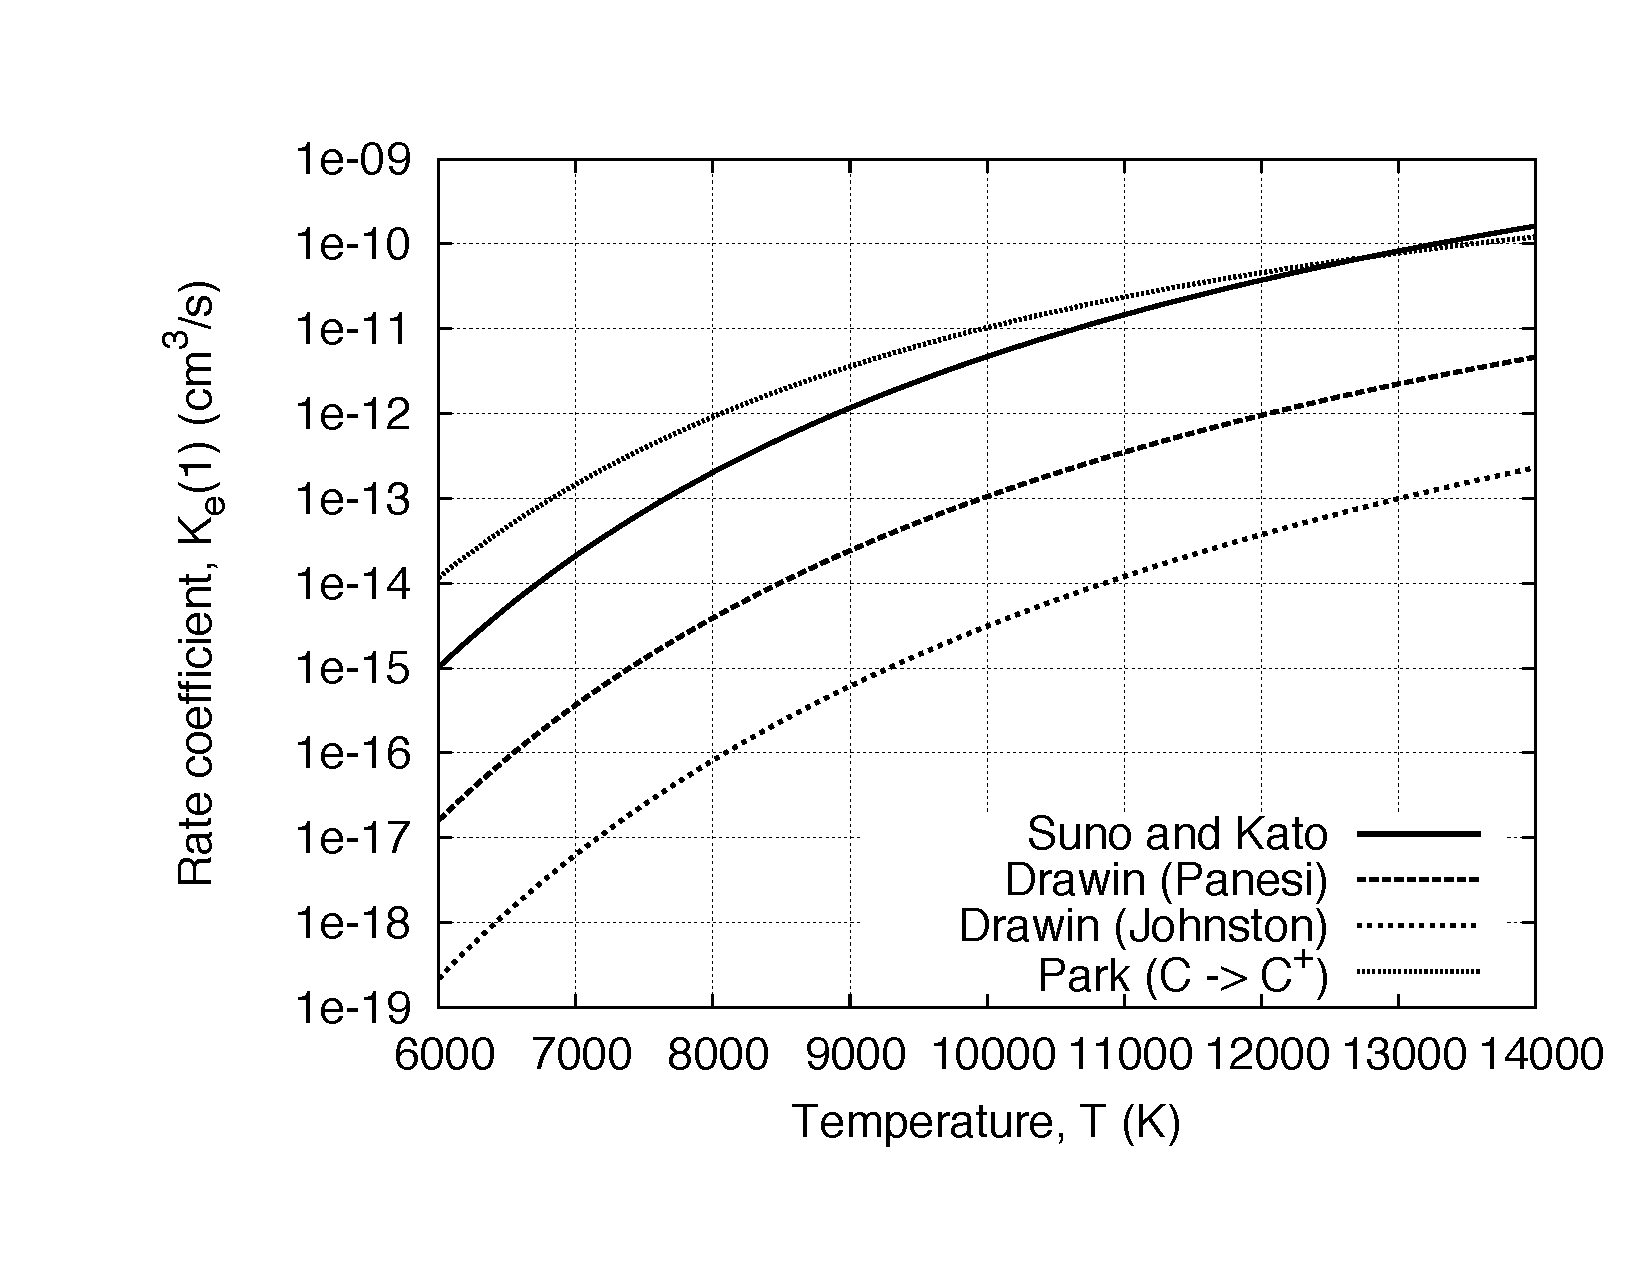
\includegraphics[width=0.48\linewidth]{collisional-radiative-modelling/figures/K_EII_C_1.pdf} \label{fig:K_EII_C_1}}
 \subfloat[$\text{C } \Clevtwo \Rightarrow \text{C}^+$]{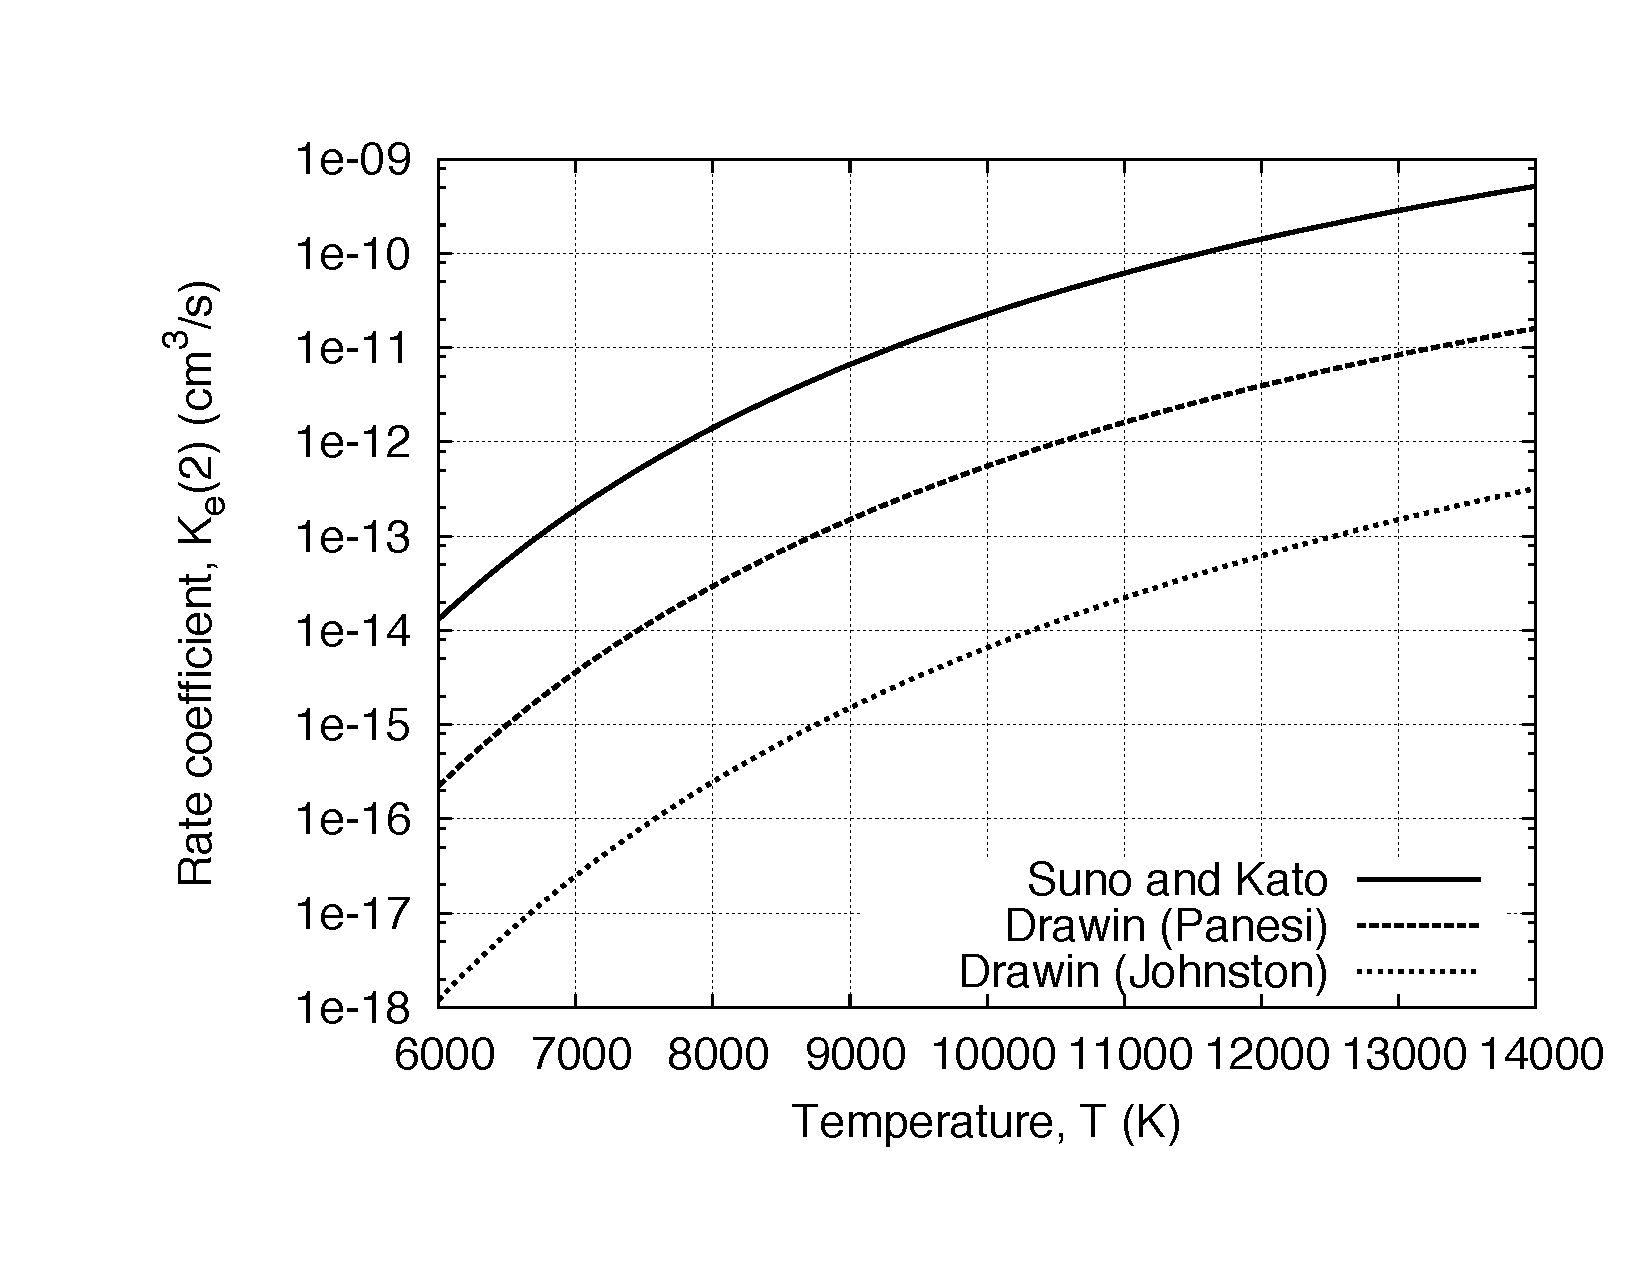
\includegraphics[width=0.48\linewidth]{collisional-radiative-modelling/figures/K_EII_C_2.pdf} \label{fig:K_EII_C_2}} \\
 \subfloat[$\text{C } \Clevthree \Rightarrow \text{C}^+$]{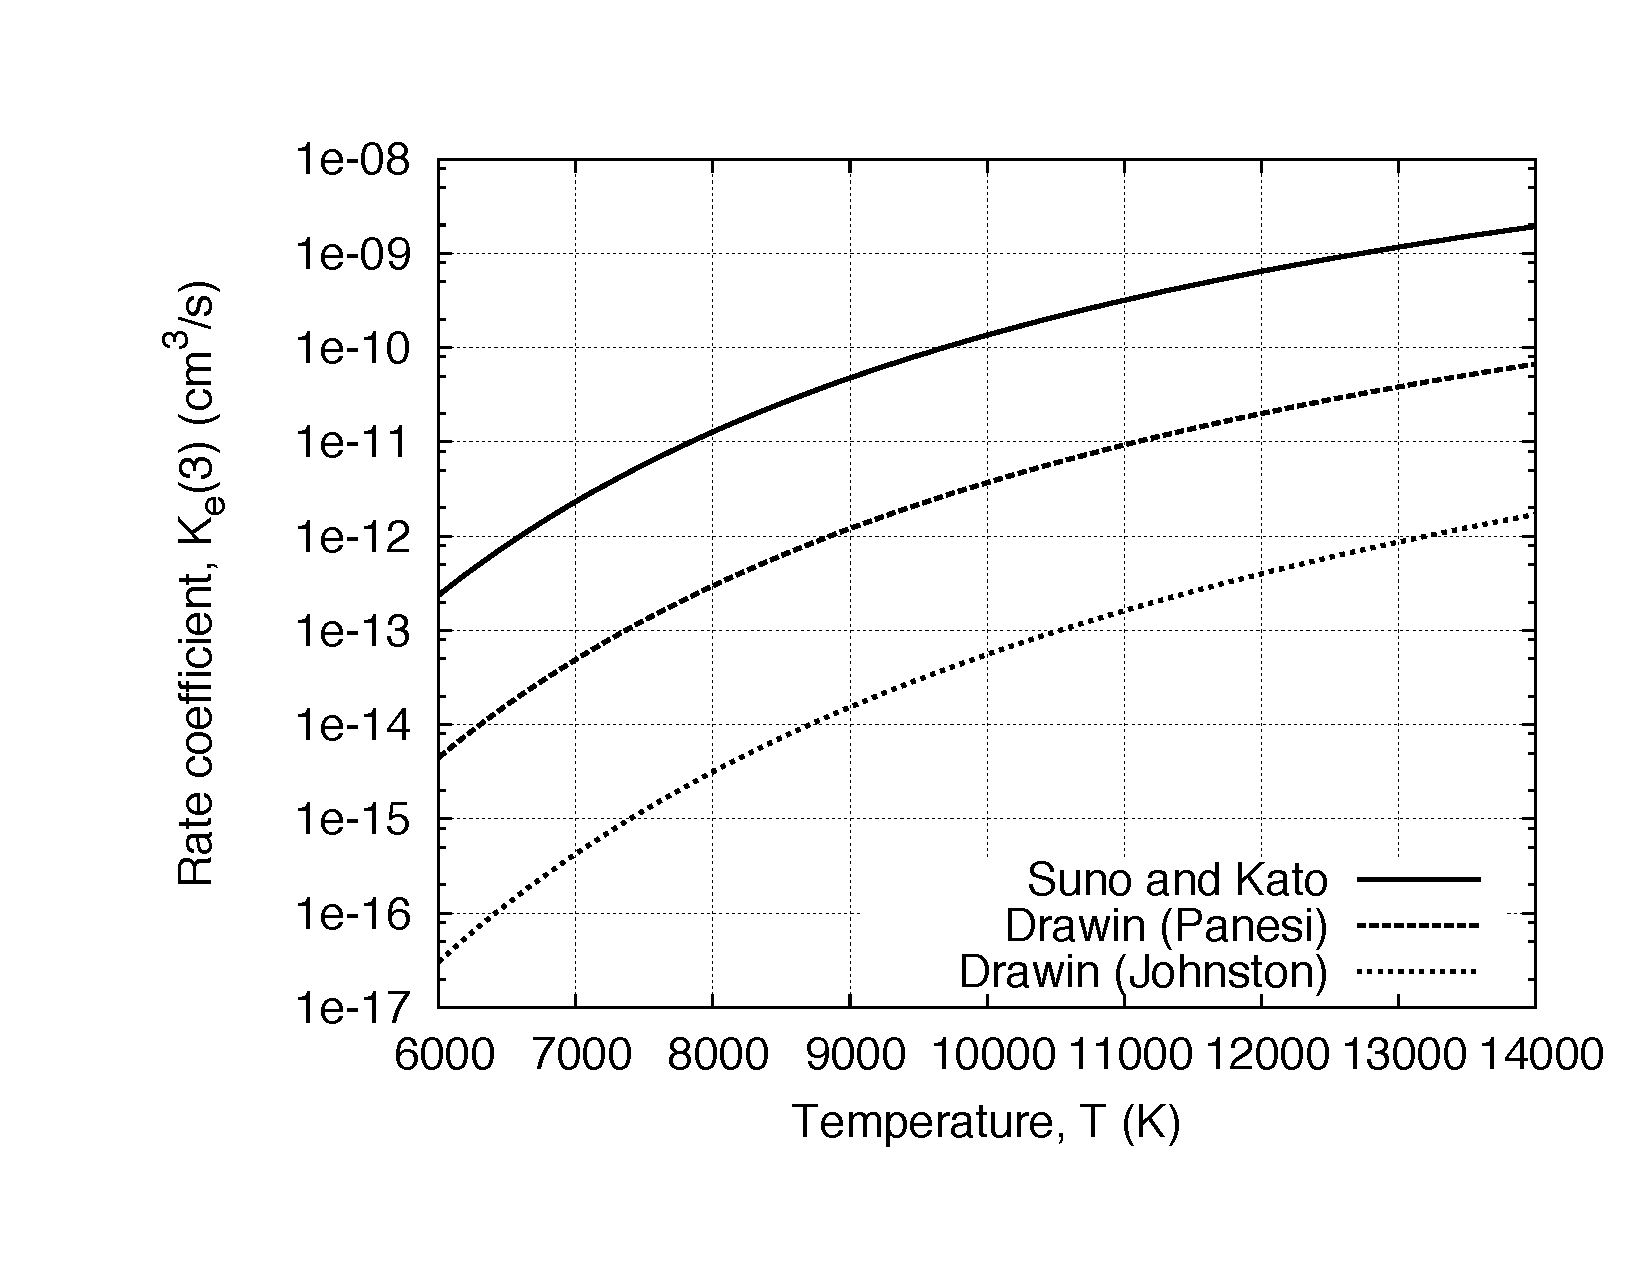
\includegraphics[width=0.48\linewidth]{collisional-radiative-modelling/figures/K_EII_C_3.pdf} \label{fig:K_EII_C_3}}
 \subfloat[$\text{C } \Clevfifteen \Rightarrow \text{C}^+$]{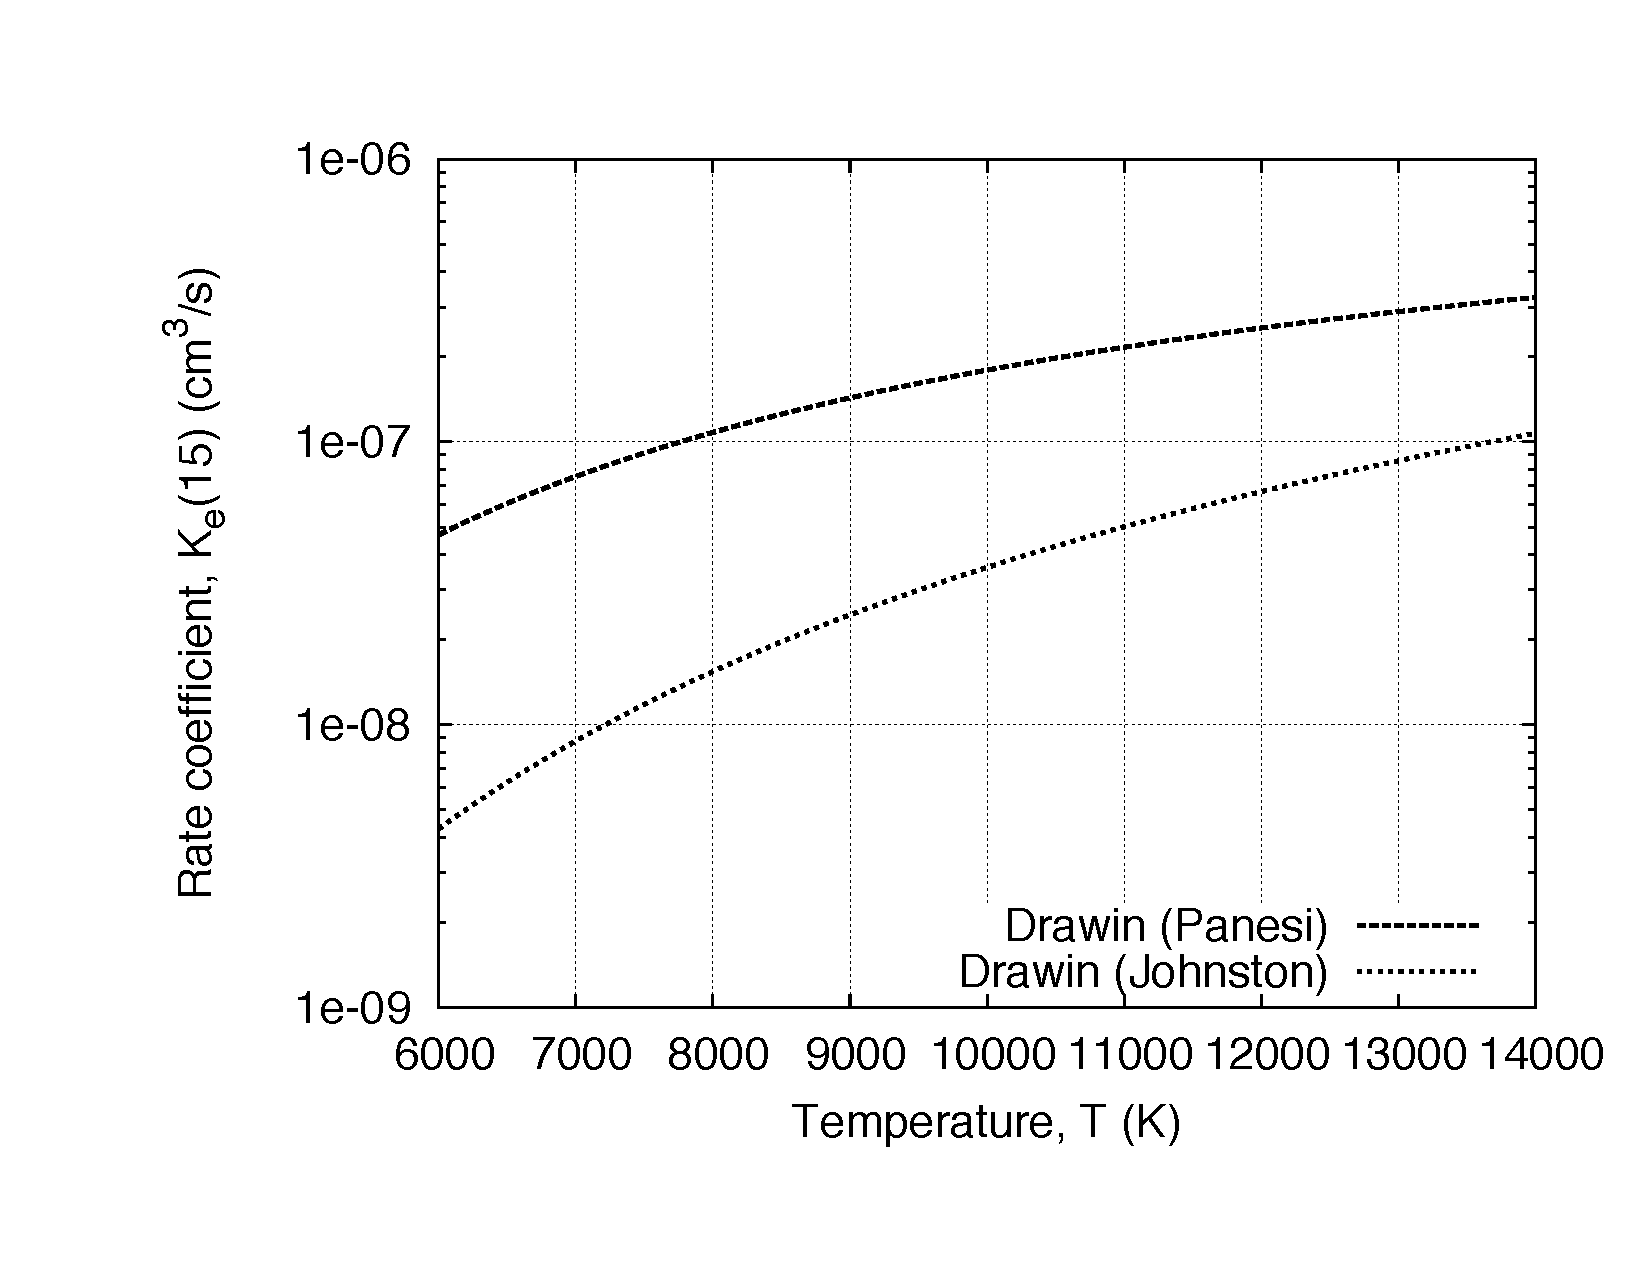
\includegraphics[width=0.48\linewidth]{collisional-radiative-modelling/figures/K_EII_C_15.pdf} \label{fig:K_EII_C_15}}
 \caption{Comparison of  electron impact ionisation rate coefficients for atomic carbon.}
 \label{fig:K_EII_C}
\end{figure}

\subsubsection{Diatomic species: C$_2$, CN and CO}

Zalogin~\cite{zalogin_2001} proposed a simple collisional-radiative model for C$_2$, CN and CO.
This model was `tuned' to match the intensity profiles measured for a 3.45\,km/s CO$_2$--N$_2$ shock tube condition, and was applied with limited success to the 8.5\,km/s CO$_2$--N$_2$ EAST shock tube condition in Reference~\cite{potter_2008c}.
Since this model was formulated, however, a set of collisional-rate coefficients and cross sections for the diatomic species CN, CO, N$_2$, N$_2^+$, O$_2$ and NO have been proposed by Park~\cite{park2008a, park2008b}.
Figure~\ref{fig:K_Park_v_Zalogin} compares the rates that are given by both Zalogin~\cite{zalogin_2001} and Park~\cite{park2008a, park2008b}.
The Zalogin model predicts faster collisional excitation of CN and slower collisional excitation of CO.
Due to large differences between some of the rates, both models will be assessed via comparison with shock tube data in~\textsection~\ref{sec:EAST_NRST}.
As the Park model is more comprehensive and based on experimental and theoretical cross sections where possible, the Park collisional excitation rates for CO and CN are tentatively accepted for inclusion in the nominal collisional-radiative models for these species.
Due to numerical difficulties encountered when implementing the heavy particle impact rates given in Reference \cite{park2008b}, however, these were omitted for CO and CN.
Considering just the electron impact processes should be sufficient for the conditions of interest due to the substantial levels of ionisation.
It should be emphasised that the heavy particle impact processes would need to be considered for the collisional-radiative model to be valid for less energetic conditions where ionisation levels are low.
The system radiative transition probabilities are calculated from the electronic-vibration transition moments via Equation~\ref{eq:A_av_diatomic}.
For C$_2$ we resort to the Zalogin~\cite{zalogin_2001} model as this species was not considered by Park in References~\cite{park2008a, park2008b}.
The nominal collisional-radiative models for C$_2$, CN and CO are summarised in \textsection~\ref{sec:C2_CR} to~\ref{sec:CO_CR} respectively.


\begin{figure}[h]
 \centering
 \subfloat[$\text{CN } \CNlevX + \text{e}^- \Longrightarrow \text{CN }\CNlevA + \text{e}^-$]{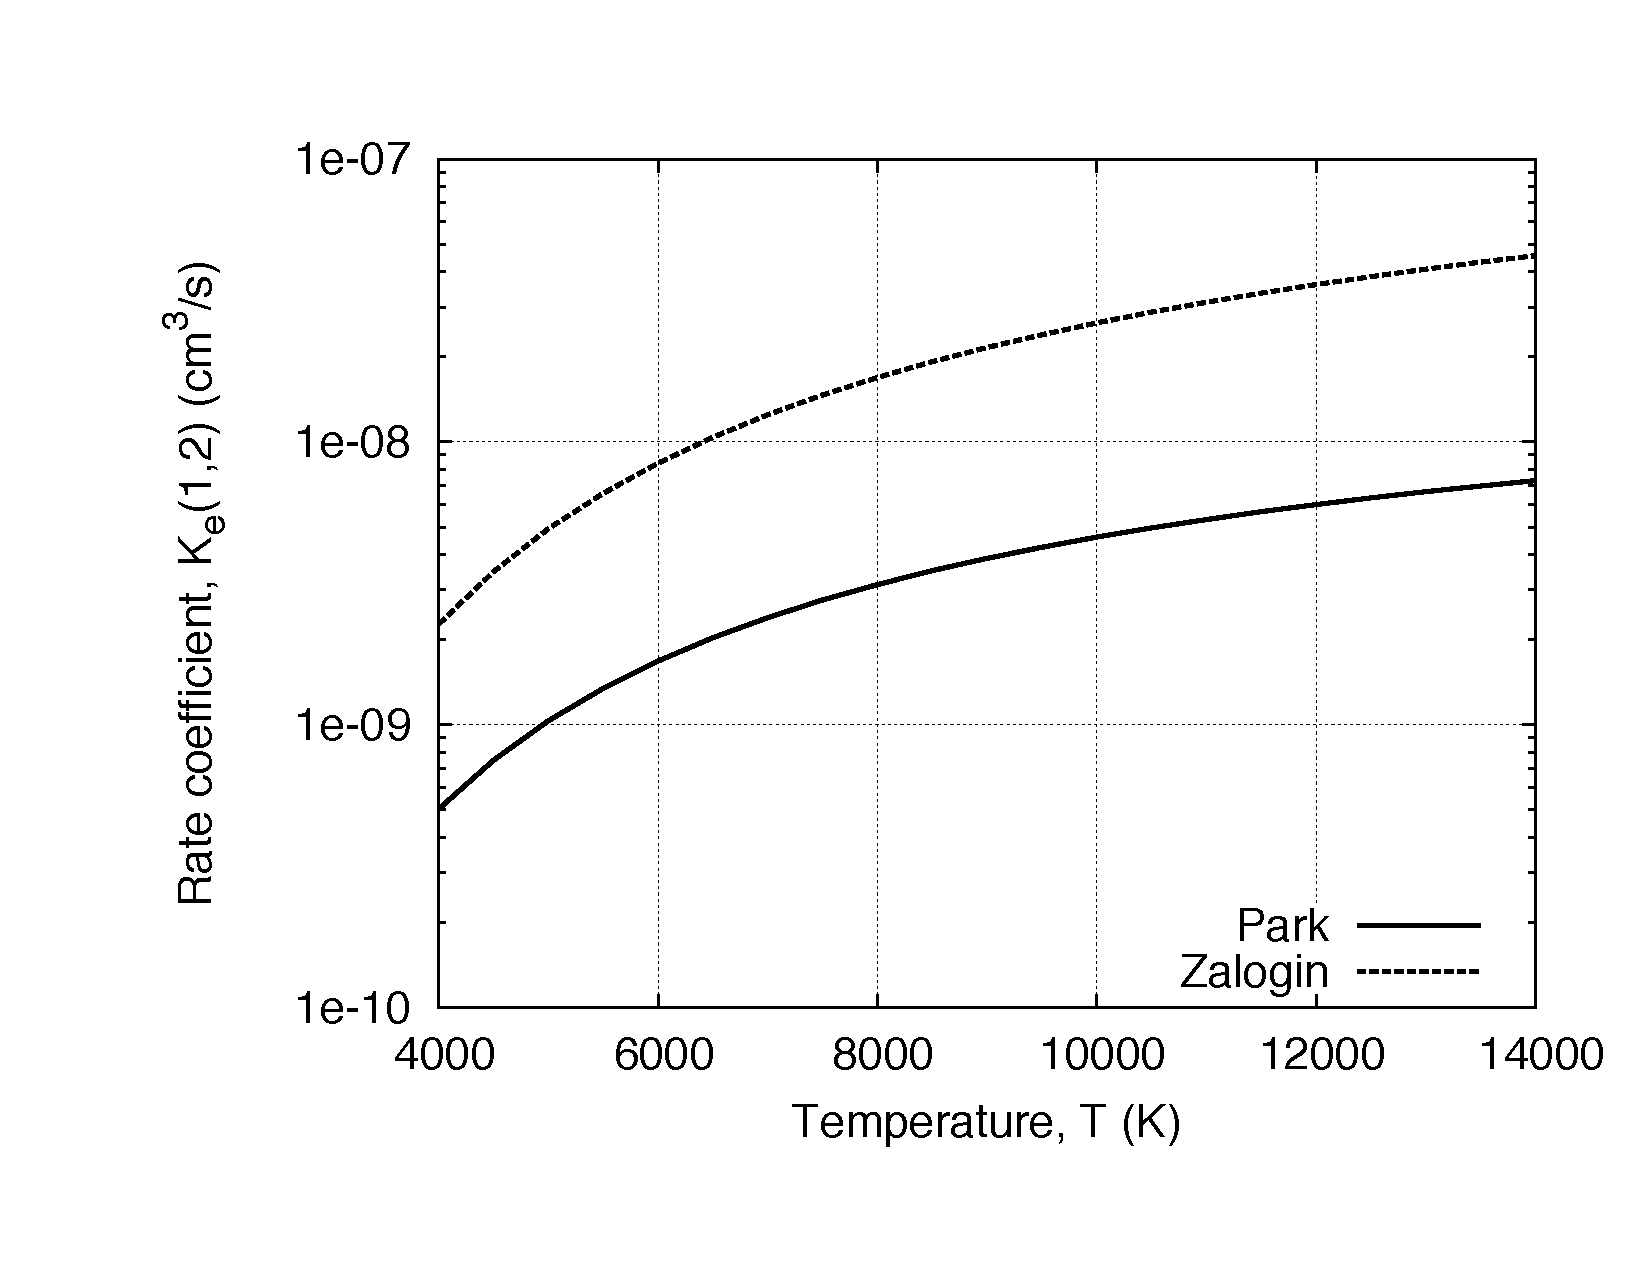
\includegraphics[width=0.48\linewidth]{collisional-radiative-modelling/figures/K_EIE_CN_X_to_A.pdf} \label{fig:K_EIE_CN_X_to_A}}
 \subfloat[$\text{CN }\CNlevX + \text{e}^- \Longrightarrow \text{CN }\CNlevB + \text{e}^-$]{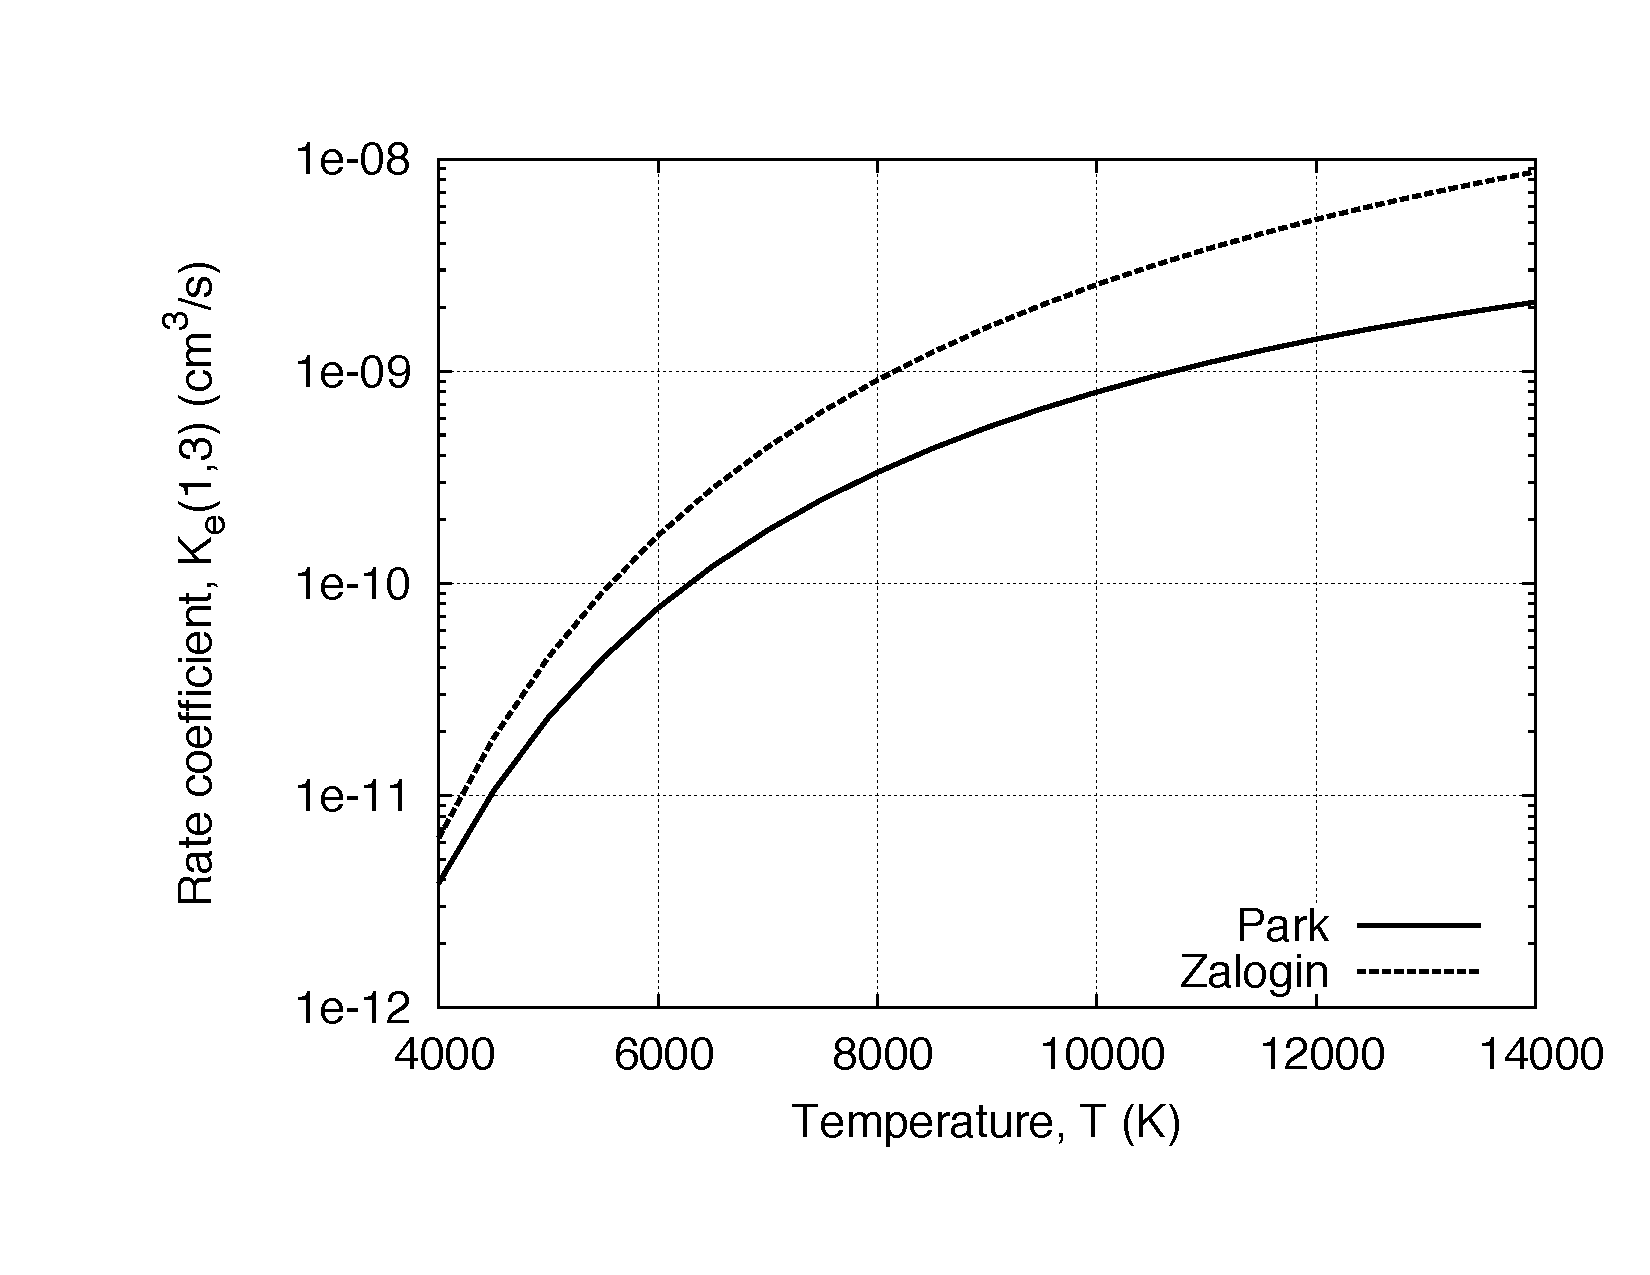
\includegraphics[width=0.48\linewidth]{collisional-radiative-modelling/figures/K_EIE_CN_X_to_B.pdf} \label{fig:K_EIE_CN_X_to_B}} \\
 \subfloat[$\text{CN }\CNlevX + \text{M}   \Longrightarrow \text{CN }\CNlevA + \text{M}$  ]{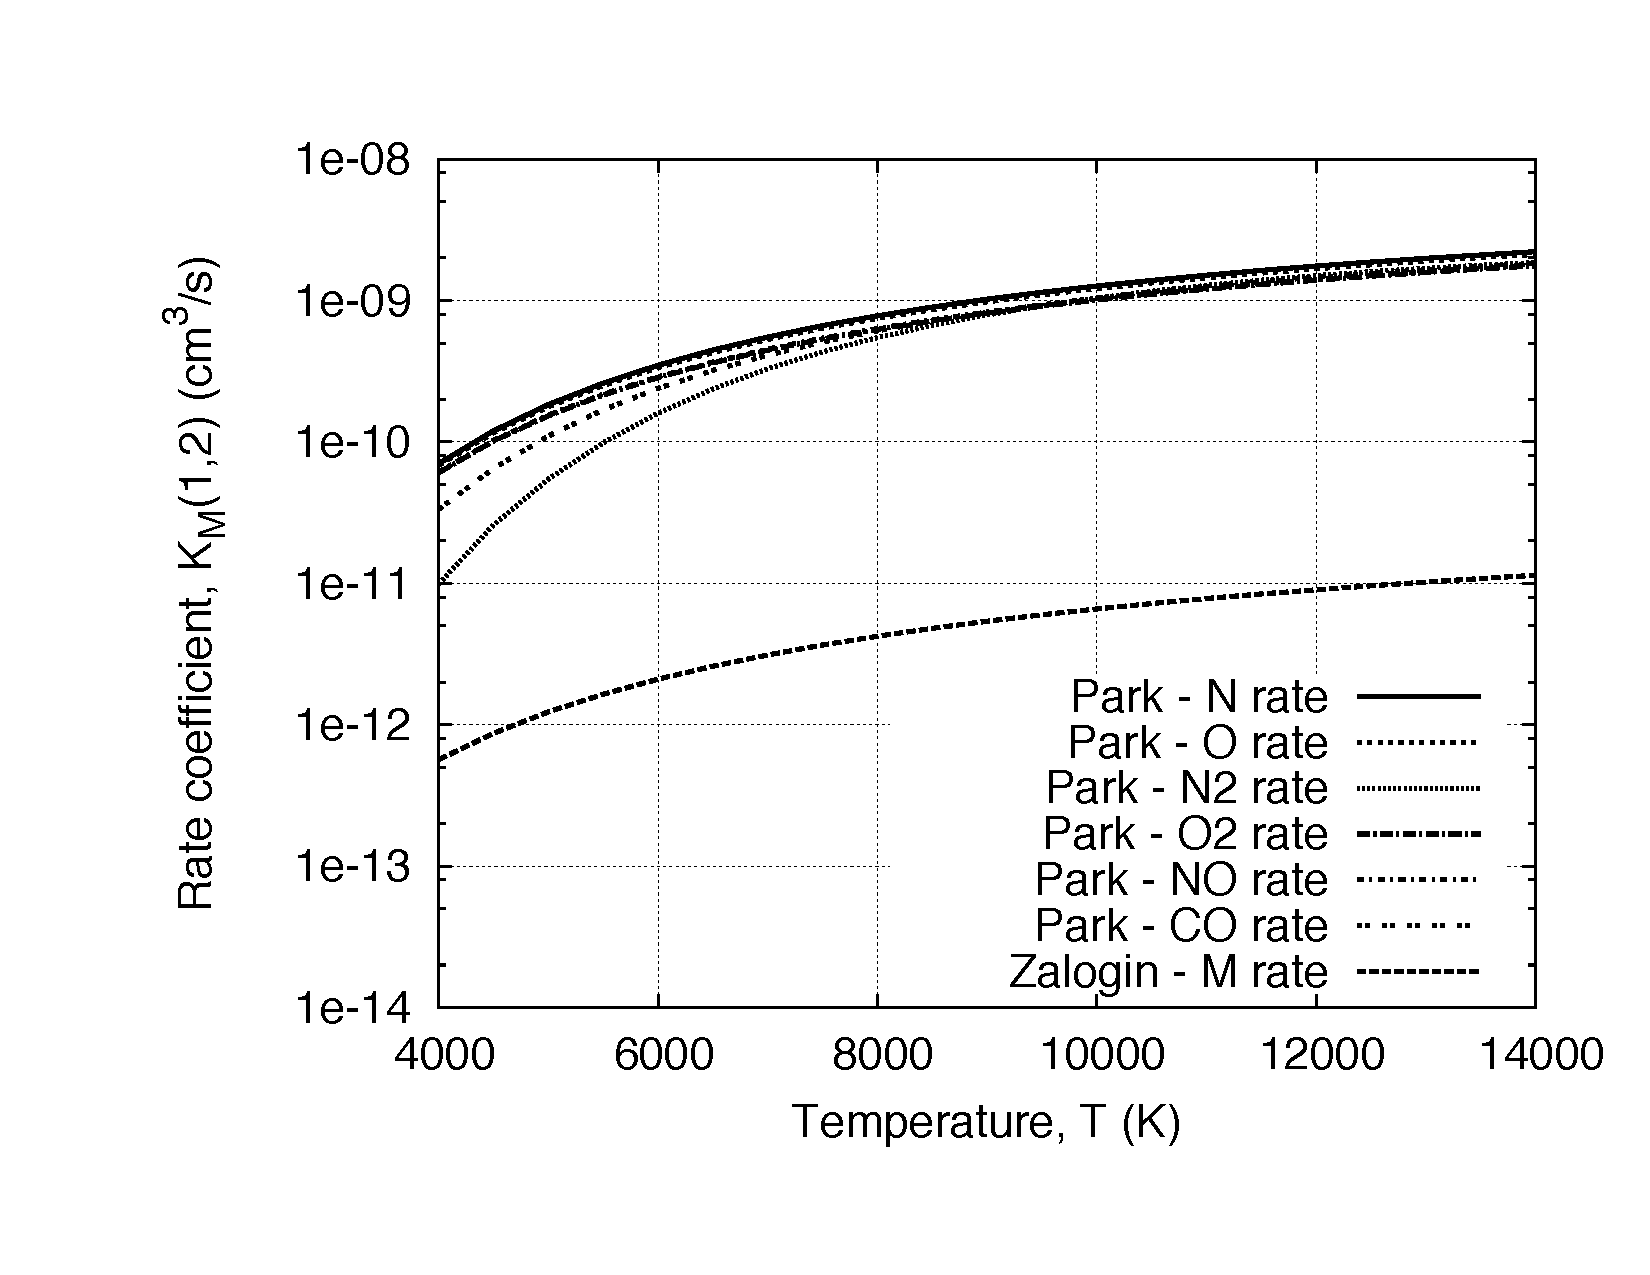
\includegraphics[width=0.48\linewidth]{collisional-radiative-modelling/figures/K_HPIE_CN_X_to_A.pdf} \label{fig:K_HPIE_CN_X_to_A}}
 \subfloat[$\text{CO }\COlevX + \text{e}^- \Longrightarrow \text{CO }\COlevA + \text{e}^- $]{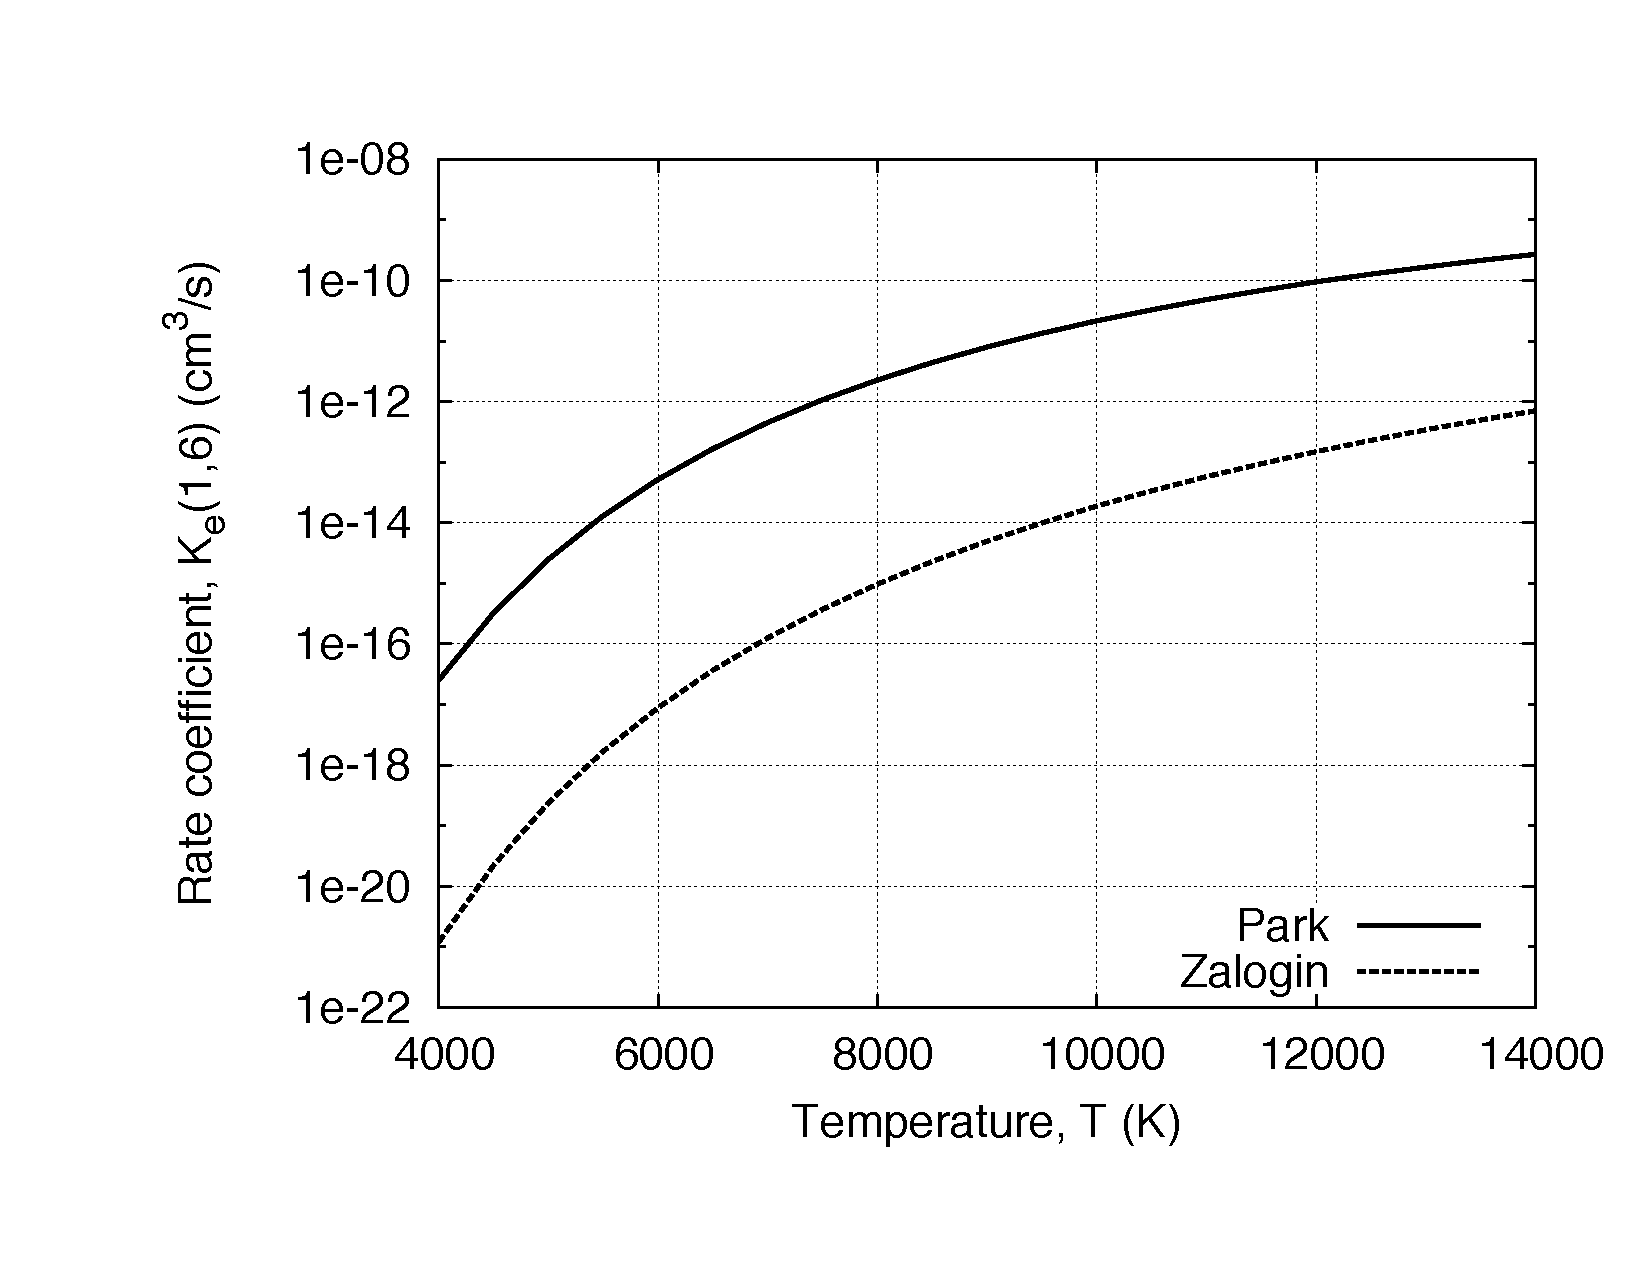
\includegraphics[width=0.48\linewidth]{collisional-radiative-modelling/figures/K_EIE_CO_X_to_A.pdf} \label{fig:K_EIE_CO_X_to_A}}
 \caption{Comparison of excitation rate coefficients obtained from Park~\cite{park2008a,park2008b} and Zalogin~\cite{zalogin_2001}.}
 \label{fig:K_Park_v_Zalogin}
\end{figure}

\subsection{A note on the selection of data sources}

In formulating the collisional-radiative model the sometimes contradictory issues of data source consistency and model accuracy arise.
On one hand, it is desirable to formulate a model that is both internally consistent (uses the same data source for all processes) and externally consistent (uses the same data sources as other models, such as the spectral radiation model).
On the other hand, it is desirable to formulate a model that best reproduces the physical phenomena.
The goal of the present work is to develop effective engineering tools, and therefore the latter approach has been preferenced to give the calculations the best chance of reproducing experimental data.
As an example, consider the electron impact excitation for the nitrogen atom.
An internally consistent model would have to use an empirical model such as that of Drawin~\cite{drawin_1968} for all transitions, however this model has been shown to give inaccurate results when applied to the excitation of low lying electronic states~\cite{panesi_2008B,panesi_phd}.
Although it breaks the internal consistency of the model, implementing the computational chemistry rates of Frost \textit{et al.}~\cite{FAS+1998} gives much improved comparisons with experiment~\cite{panesi_2008B,panesi_phd}.
This principal of selecting the most effective data, rather than the most consistent data, has been applied throughout the collisional-radiative model.


